\begin{frame}[t]{}
\relax
\vspace{.55cm}{\fontsize{30}{34}\selectfont\color{IEEEBlue}\bfseries Agentic AI for\\Utility Operators}\par\vspace{.38cm}
{\large Real power-sector uses, engineering tools and measured research results}\par\medskip
{\large 165 minutes / two worked exercises}\par\medskip
\medskip\begin{columns}[T,onlytextwidth]
\begin{column}{.48\textwidth}{\large\bfseries Alaa Selim\par}{\normalsize MIT/Dartmouth\par}\end{column}
\begin{column}{.48\textwidth}{\large\bfseries Mohamed Chehada\par}{\normalsize UT Austin\par}\end{column}
\end{columns}\medskip
\vfill
\includegraphics[width=4cm]{images/comsoc-lockup.png}\par{\tiny Independent educational material / IEEE ComSoc theme adaptation}
\vfill
{\fontsize{6.3}{7.5}\selectfont\color{Slate} Source: \href{https://www.comsoc.org/about/brand-experience/resources}{IEEE Communications Society. IEEE Communications Society: official resources and network presentation template. Reviewed 17 October 2026.}\par}
\note{All slides belong to the main presentation. The opening distinguishes systems in use, utility statements and product announcements. Every agent-research paper covers a power-system task. We explain LangGraph and task dependency graphs through fault analysis and weather-risk studies. A separate follow-on workshop covers the detailed GridGuard cases on voltage, restoration and cyber events. Takeaway: 

IEEE Communications Society. IEEE Communications Society: official resources and network presentation template. Reviewed 17 October 2026.
Full source: https://www.comsoc.org/about/brand-experience/resources}
\end{frame}

\begin{frame}[t]{What is agentic AI?}
\relax
\begingroup\centering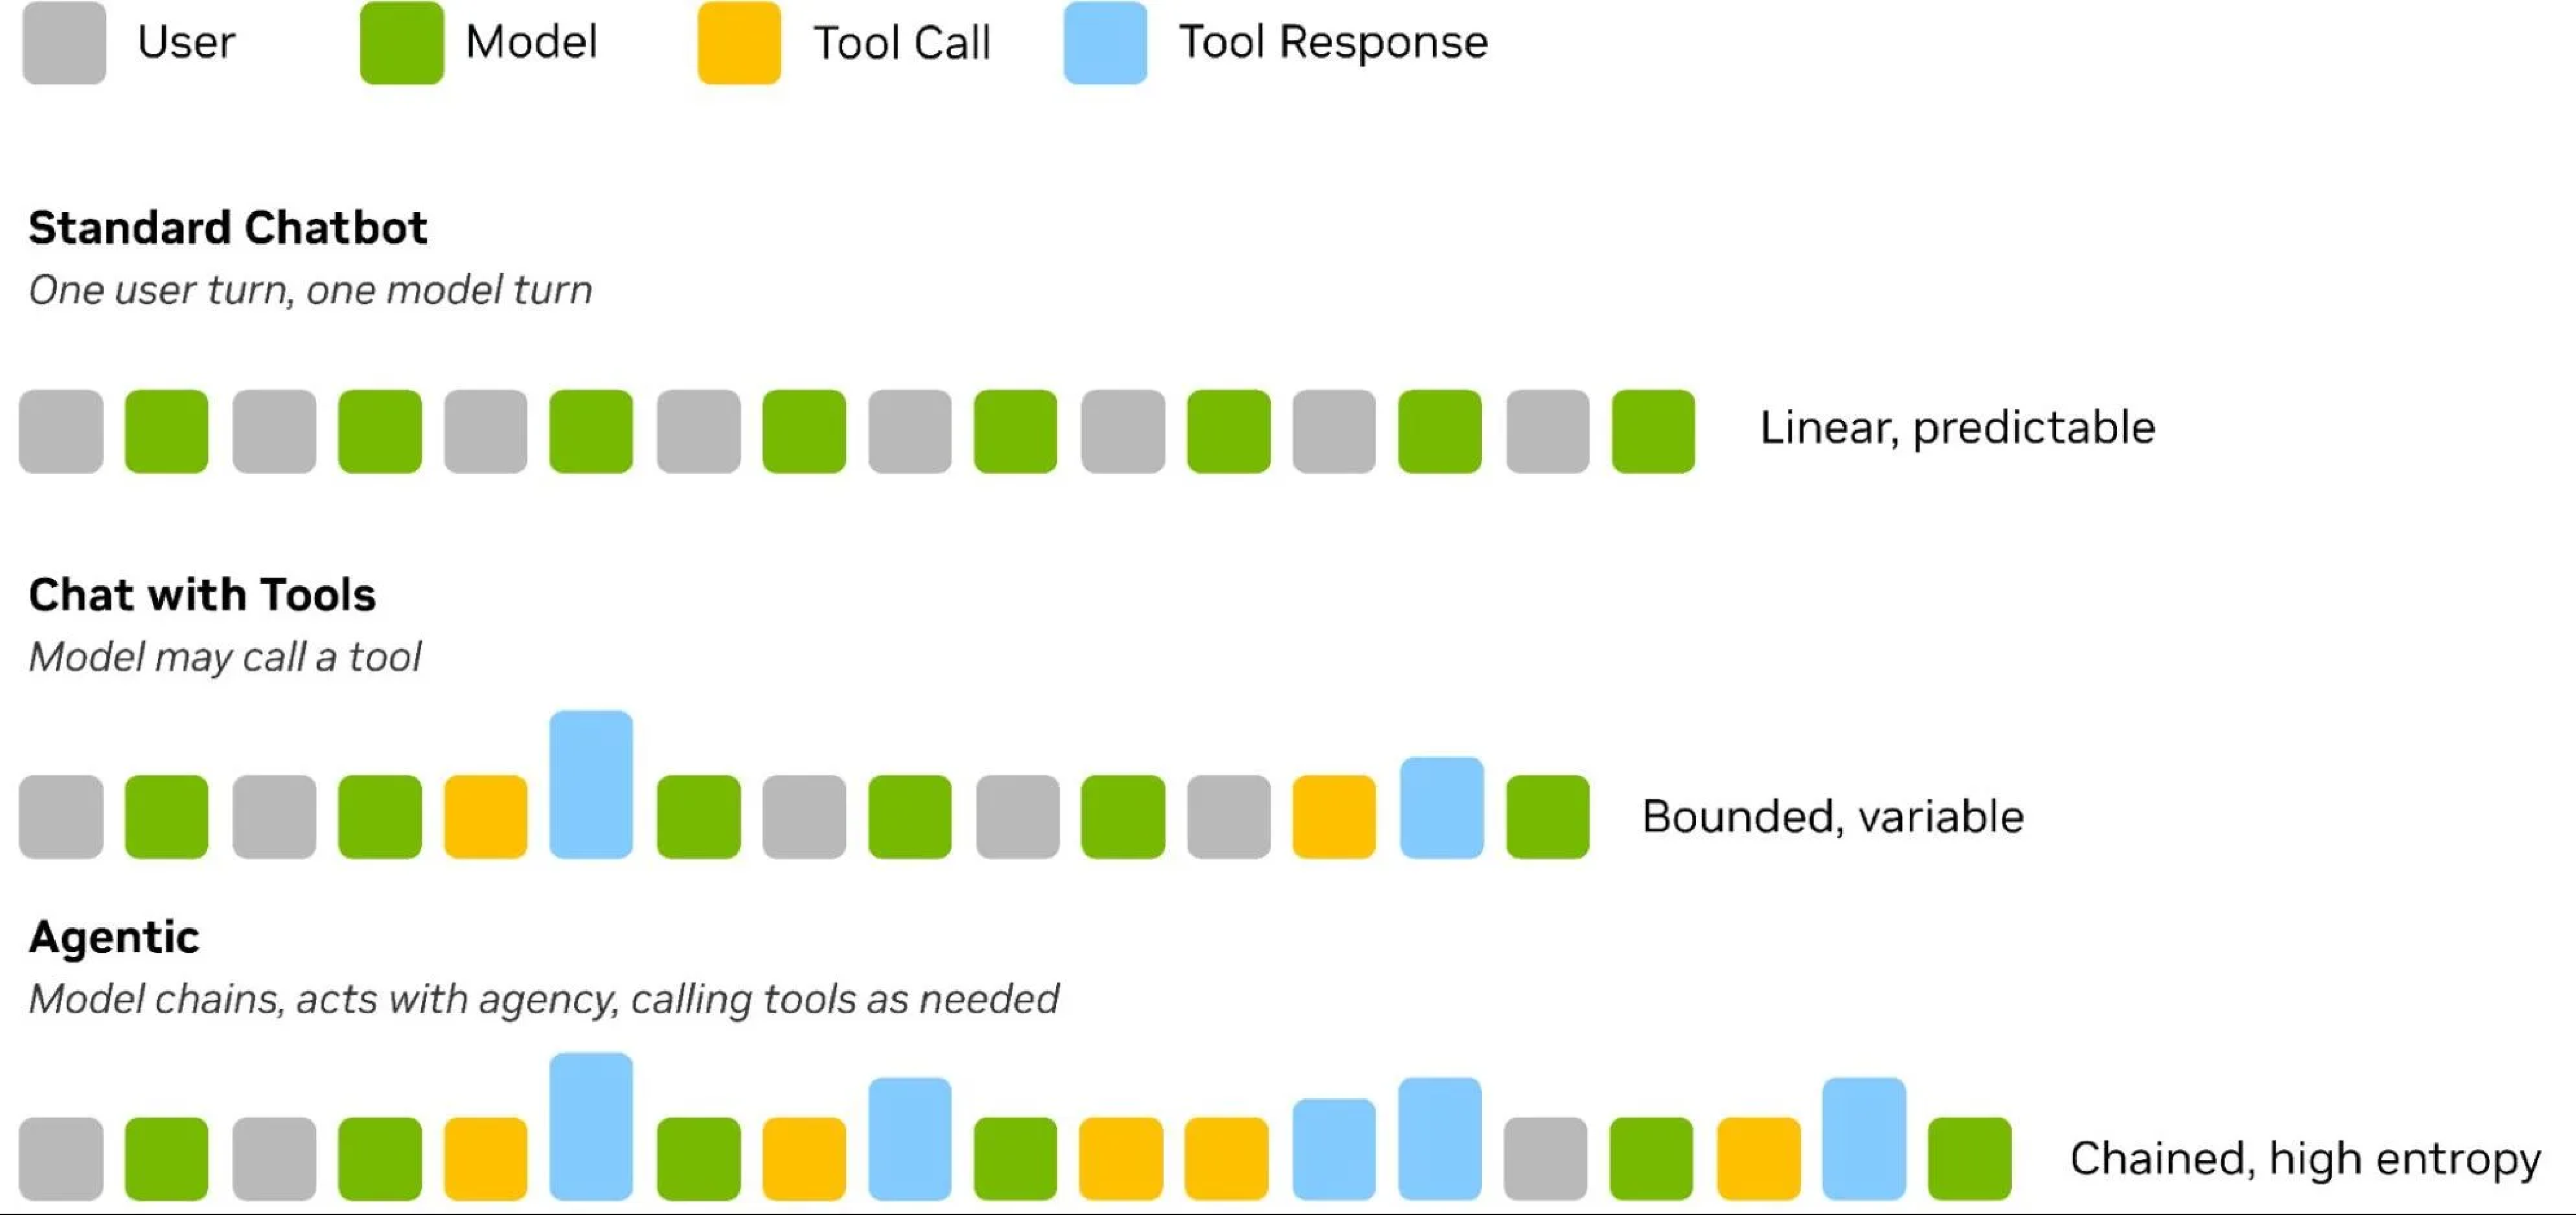
\includegraphics[width=\linewidth,height=4.3cm,keepaspectratio]{images/real_framework_nvidia_interaction_patterns.pdf}
\par{\fontsize{7}{8.3}\selectfont\color{Slate} Original NVIDIA interaction patterns. The same generative model can be part of a chat or an agentic system.}
\par\endgroup\smallskip
{
\small\begin{itemize}
\setlength{\itemsep}{.25em}
\item An agentic system uses feedback to choose and adjust actions toward a goal. One agent may be enough.
\end{itemize}\par}
\vfill
{\fontsize{6.3}{7.5}\selectfont\color{Slate} Source: \href{https://www.anthropic.com/engineering/building-effective-agents}{Erik S., Barry Zhang. Building effective agents. Anthropic Engineering. 2024-12-19.}\par}
\note{The first sentence is our summary, not a quotation or a standard definition. Anthropic includes both programmed workflows and LLM-directed agents under agentic systems. Wooldridge and Jennings also discuss different definitions of an agent. The later examples focus on engineering systems using large language models, or LLMs. "Agentic" describes how the whole system pursues a task. It is not another software component beside the agent. A system can use just one agent. Source: NVIDIA Technical Blog, Figure 1. The three examples show interaction patterns, not a universal taxonomy or a claim that tool use alone proves autonomy. Source figure locator: Figure 1. Original source URL: https://developer.nvidia.com/blog/building-for-the-rising-complexity-of-agentic-systems-with-extreme-co-design/ Takeaway: 

Erik S., Barry Zhang. Building effective agents. Anthropic Engineering. 2024-12-19.
Full source: https://www.anthropic.com/engineering/building-effective-agents

Michael Wooldridge, Nicholas R. Jennings. Intelligent agents: theory and practice. The Knowledge Engineering Review, 10(2), pp. 115--152. 1995.
Full source: https://doi.org/10.1017/S0269888900008122
Full paper: https://www.cs.ox.ac.uk/people/michael.wooldridge/pubs/ker95.pdf

Eduardo Alvarez, Benjamin Klieger, Graham Steele. Building for the Rising Complexity of Agentic Systems with Extreme Co-Design. NVIDIA Technical Blog. May 5, 2026.
Full source: https://developer.nvidia.com/blog/building-for-the-rising-complexity-of-agentic-systems-with-extreme-co-design/}
\end{frame}

\begin{frame}[t]{Generative AI creates content}
\relax
\begingroup\begin{minipage}[c][3.8cm][c]{\linewidth}\centering\setbox0=\hbox{\resizebox{.96\linewidth}{!}{\begin{tikzpicture}[x=1cm,y=1cm,font=\sffamily\fontsize{12}{14}\selectfont,
  line cap=round,line join=round,
  rp/.style={circle,draw=rBlue,fill=white,minimum size=5.4mm,inner sep=0pt,line width=1.15pt},
  rl/.style={align=center,text=rNavy,font=\sffamily\bfseries\fontsize{12.5}{14.5}\selectfont},
  rn/.style={align=center,text=rNavy,font=\sffamily\fontsize{11.2}{13}\selectfont},
  rc/.style={align=left,text=rNavy,font=\ttfamily\fontsize{11}{13}\selectfont},
  rf/.style={-{Latex[length=2mm,width=1.5mm]},draw=rBlue,line width=1.15pt,shorten >=1.4pt,shorten <=1.4pt},
  rw/.style={-{Latex[length=2mm,width=1.5mm]},draw=rOrange,line width=1.15pt,shorten >=1.4pt,shorten <=1.4pt}]
\definecolor{rBlue}{HTML}{00629B}
\definecolor{rCyan}{HTML}{00A8C8}
\definecolor{rNavy}{HTML}{003B5C}
\definecolor{rOrange}{HTML}{B65B14}
\definecolor{rGray}{HTML}{74828C}
\path[use as bounding box] (0,0) rectangle (14.2,4.2);

\node[rp] (prompt) at (1.6,3.0) {};
\node[rl] at (1.6,3.7) {Prompt};
\node[rp] (records) at (1.6,1.05) {};
\node[rl] at (1.6,1.83) {Selected\\records};
\coordinate (join) at (4.1,2.05);
\draw[draw=rBlue,line width=1.15pt] (prompt.east) -- (4.1,3.0) -- (join);
\draw[draw=rBlue,line width=1.15pt] (records.east) -- (4.1,1.05) -- (join);
\fill[rBlue] (join) circle (1.7pt);
\node[rp] (model) at (7.0,2.05) {};
\node[rl] at (7.0,3.02) {Generative\\model};
\draw[rf] (join) -- (model.west);
\node[rp] (draft) at (12.15,2.05) {};
\node[rl] at (12.15,2.83) {Draft report};
\node[rn] at (12.15,1.36) {content to review};
\draw[rf] (model.east) -- (draft.west);

\end{tikzpicture}
}}\ifdim\dimexpr\ht0+\dp0\relax>3.8cm\resizebox{!}{3.8cm}{\box0}\else\box0\fi\par\end{minipage}
{\fontsize{7}{8.3}\selectfont\color{Slate} Illustrative report-drafting example. Generative models can also be components of agents.\par}
\endgroup\smallskip
{
\small\begin{itemize}
\setlength{\itemsep}{.25em}
\item Generative AI makes text, images and other content. Large language models (LLMs) are used for text.
\item A single call can create a draft. An agent system can use the same model to choose steps.
\end{itemize}\par}
\vfill
{\fontsize{6.3}{7.5}\selectfont\color{Slate} Source: \href{https://doi.org/10.6028/NIST.AI.600-1}{National Institute of Standards and Technology. Artificial Intelligence Risk Management Framework: Generative Artificial Intelligence Profile. NIST AI 600-1. July 2024.}\par}
\note{NIST AI 600-1 describes generative AI in terms of producing synthetic content, including text, images, audio and other media. This diagram shows one generation call: selected records and a request enter a model, which produces a draft. It does not say every generative-AI application is a single call. An LLM-based agent can use a generative model inside a repeated decision process. These categories describe different roles, not three mutually exclusive technologies or stages of a historical evolution. Generated wording is not itself numerical grid evidence; a study report should cite the engineering records used. Takeaway: 

National Institute of Standards and Technology. Artificial Intelligence Risk Management Framework: Generative Artificial Intelligence Profile. NIST AI 600-1. July 2024.
Full source: https://doi.org/10.6028/NIST.AI.600-1
Full paper: https://nvlpubs.nist.gov/nistpubs/ai/NIST.AI.600-1.pdf

Erik S., Barry Zhang. Building effective agents. Anthropic Engineering. 2024-12-19.
Full source: https://www.anthropic.com/engineering/building-effective-agents}
\end{frame}

\begin{frame}[t]{What is an AI agent?}
\relax
\begin{columns}[T,onlytextwidth]\begin{column}{.64\textwidth}
\begingroup\centering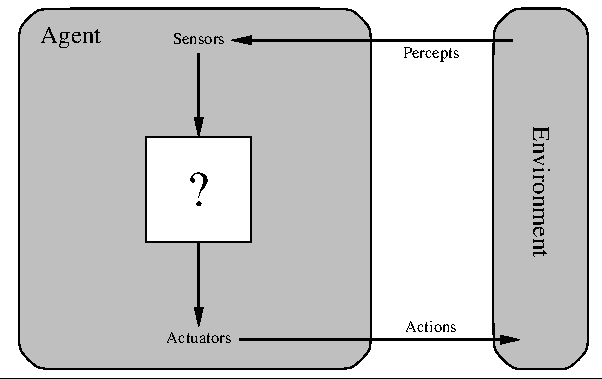
\includegraphics[width=\linewidth,height=4.65cm,keepaspectratio]{images/real_concept_classical_agent.pdf}
\par{\fontsize{7}{8.3}\selectfont\color{Slate} Russell and Norvig's original agent diagram, Figure 2.1. A software agent's sensors and actuators can be software interfaces.}
\par\endgroup\smallskip
\end{column}\begin{column}{.32\textwidth}
{
\small\begin{itemize}
\setlength{\itemsep}{.25em}
\item An agent observes an environment and chooses actions that affect it.
\item In a study, an engineering solver calculates grid behavior. The agent reads its results and chooses the next tool call.
\end{itemize}\par}
\end{column}\end{columns}
\vfill
{\fontsize{6.3}{7.5}\selectfont\color{Slate} Source: \href{https://aima.cs.berkeley.edu/2nd-ed/}{Stuart J. Russell, Peter Norvig. Artificial Intelligence: A Modern Approach, Chapter 2: Intelligent Agents. Prentice Hall, second edition, Chapter 2, pp. 32--58. 2003.}\par}
\note{The equation is teaching notation: the policy uses the history of observations to choose the next action. It is not the textbook's exact notation. The agent function is this abstract mapping, and a program implements it. A grid-study agent may observe case files and solver logs, then call a tool, ask for information or return a report. This classical definition predates LLMs. It also includes many older forms of automation. The linked sample chapter is from the second edition, even though its URL says fourth edition. The reading guide records that difference. Teaching notation: a\_t = pi(o\_1, ..., o\_t), a rule mapping past observations to the next action. The original textbook figure replaces the teaching redraw. The question mark represents the agent's decision mechanism; observations enter through sensors and actions leave through actuators. This is the author-hosted older chapter draft, cited as second edition. Takeaway: 

Stuart J. Russell, Peter Norvig. Artificial Intelligence: A Modern Approach, Chapter 2: Intelligent Agents. Prentice Hall, second edition, Chapter 2, pp. 32--58. 2003.
Full source: https://aima.cs.berkeley.edu/2nd-ed/
Full paper: https://aima.cs.berkeley.edu/4th-ed/pdfs/newchap02.pdf}
\end{frame}

\begin{frame}[t]{An agent chooses a step. A tool runs it.}
\relax
\begin{columns}[T,onlytextwidth]\begin{column}{.64\textwidth}
\begingroup\centering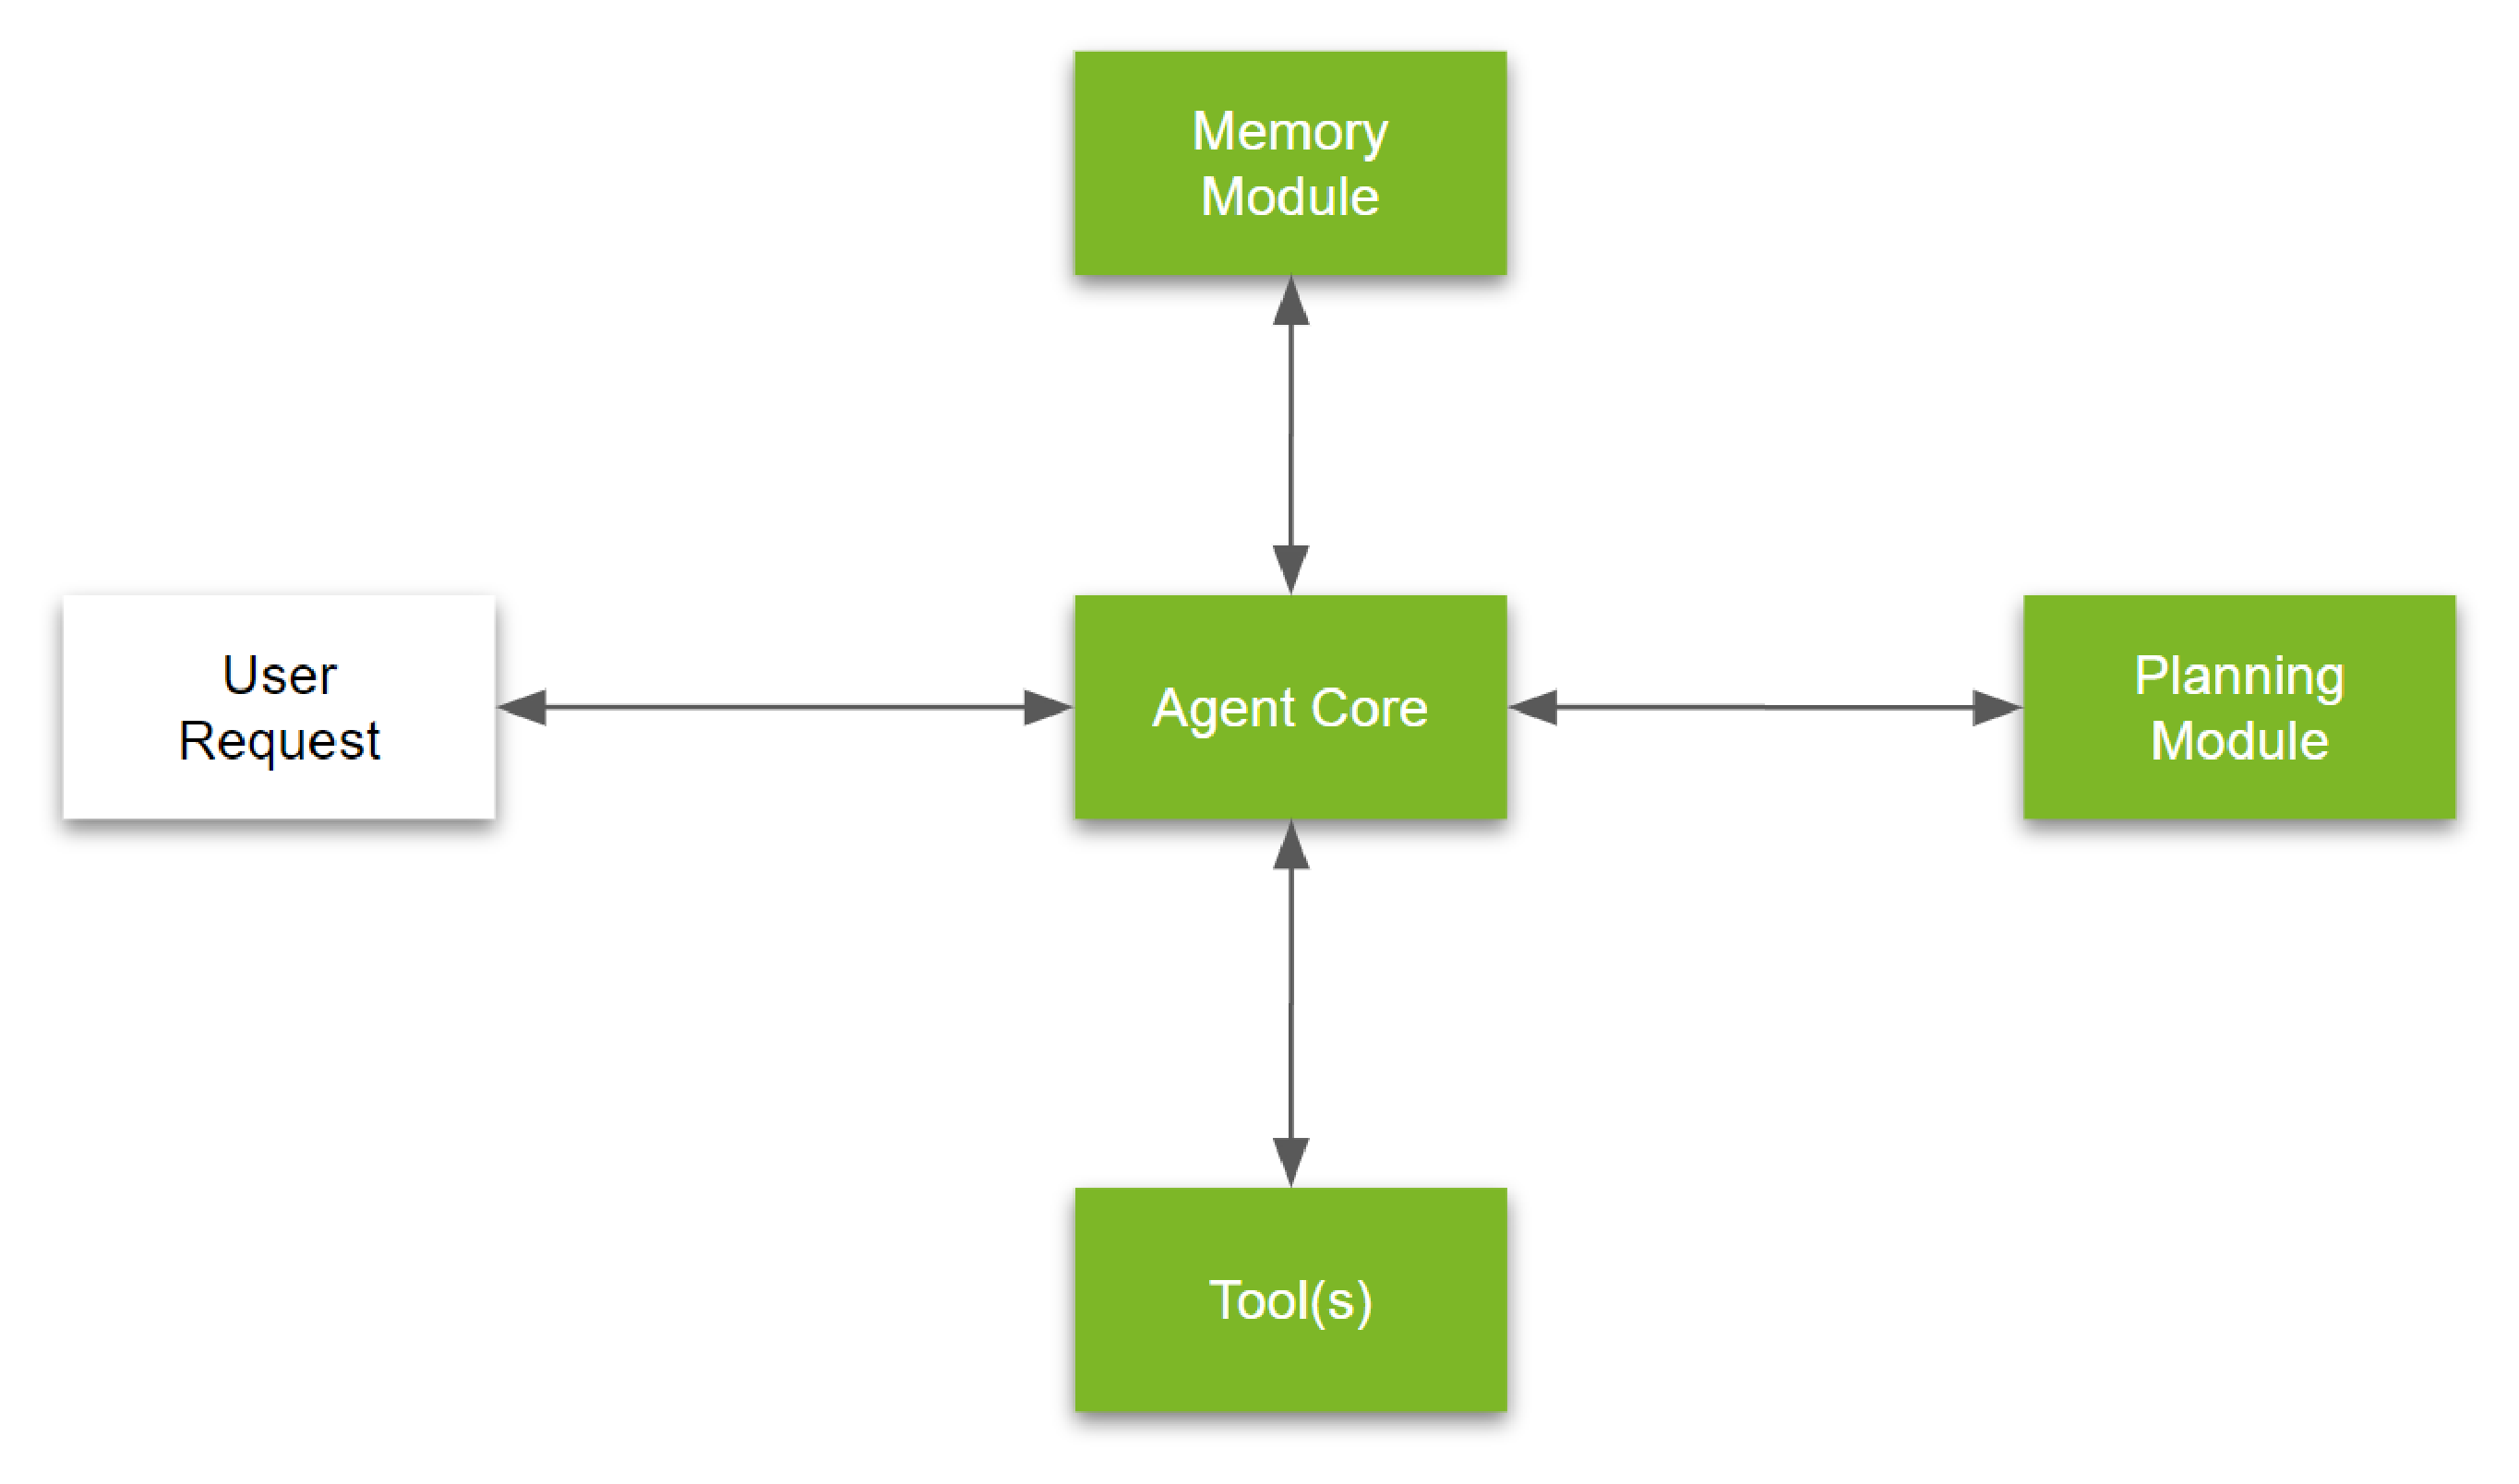
\includegraphics[width=\linewidth,height=4.65cm,keepaspectratio]{images/real_framework_nvidia_agent_components.pdf}
\par{\fontsize{7}{8.3}\selectfont\color{Slate} Original NVIDIA agent design: the core connects a request with tools, planning and memory. Other designs can combine these roles.}
\par\endgroup\smallskip
\end{column}\begin{column}{.32\textwidth}
{
\small\begin{itemize}
\setlength{\itemsep}{.25em}
\item The agent chooses an allowed step. A tool carries out the request.
\item An engineering solver calculates grid behavior. The agent uses the returned evidence.
\end{itemize}\par}
\end{column}\end{columns}
\vfill
{\fontsize{6.3}{7.5}\selectfont\color{Slate} Source: \href{https://developer.nvidia.com/blog/introduction-to-llm-agents/}{Tanay Varshney. Introduction to LLM Agents. NVIDIA Technical Blog. November 30, 2023.}\par}
\note{A run\_pf request should identify the study case. Its response should include status, numerical results and an evidence ID. The solver computes the electrical result. After an error, an LLM may choose another allowed check or stop and ask for help. The runtime software saves progress and carries out those choices. This example gives no permission to switch live equipment. A service may contain its own agents and still act as a tool for the agent calling it. Source: NVIDIA Technical Blog, Figure 1. This is a published conceptual design; separate memory or planning modules are not required in every AI agent. Source figure locator: Figure 1: General components of an agent. Original source URL: https://developer.nvidia.com/blog/introduction-to-llm-agents/ Takeaway: 

LangChain maintainers. Tools. Docs by LangChain, Python open-source documentation. Accessed 17 October 2026.
Full source: https://docs.langchain.com/oss/python/langchain/tools

Erik S., Barry Zhang. Building effective agents. Anthropic Engineering. 2024-12-19.
Full source: https://www.anthropic.com/engineering/building-effective-agents

Stuart J. Russell, Peter Norvig. Artificial Intelligence: A Modern Approach, Chapter 2: Intelligent Agents. Prentice Hall, second edition, Chapter 2, pp. 32--58. 2003.
Full source: https://aima.cs.berkeley.edu/2nd-ed/
Full paper: https://aima.cs.berkeley.edu/4th-ed/pdfs/newchap02.pdf

Tanay Varshney. Introduction to LLM Agents. NVIDIA Technical Blog. November 30, 2023.
Full source: https://developer.nvidia.com/blog/introduction-to-llm-agents/}
\end{frame}

\begin{frame}[t]{Workflow or agent: who chooses the next step?}
\relax
\begingroup\centering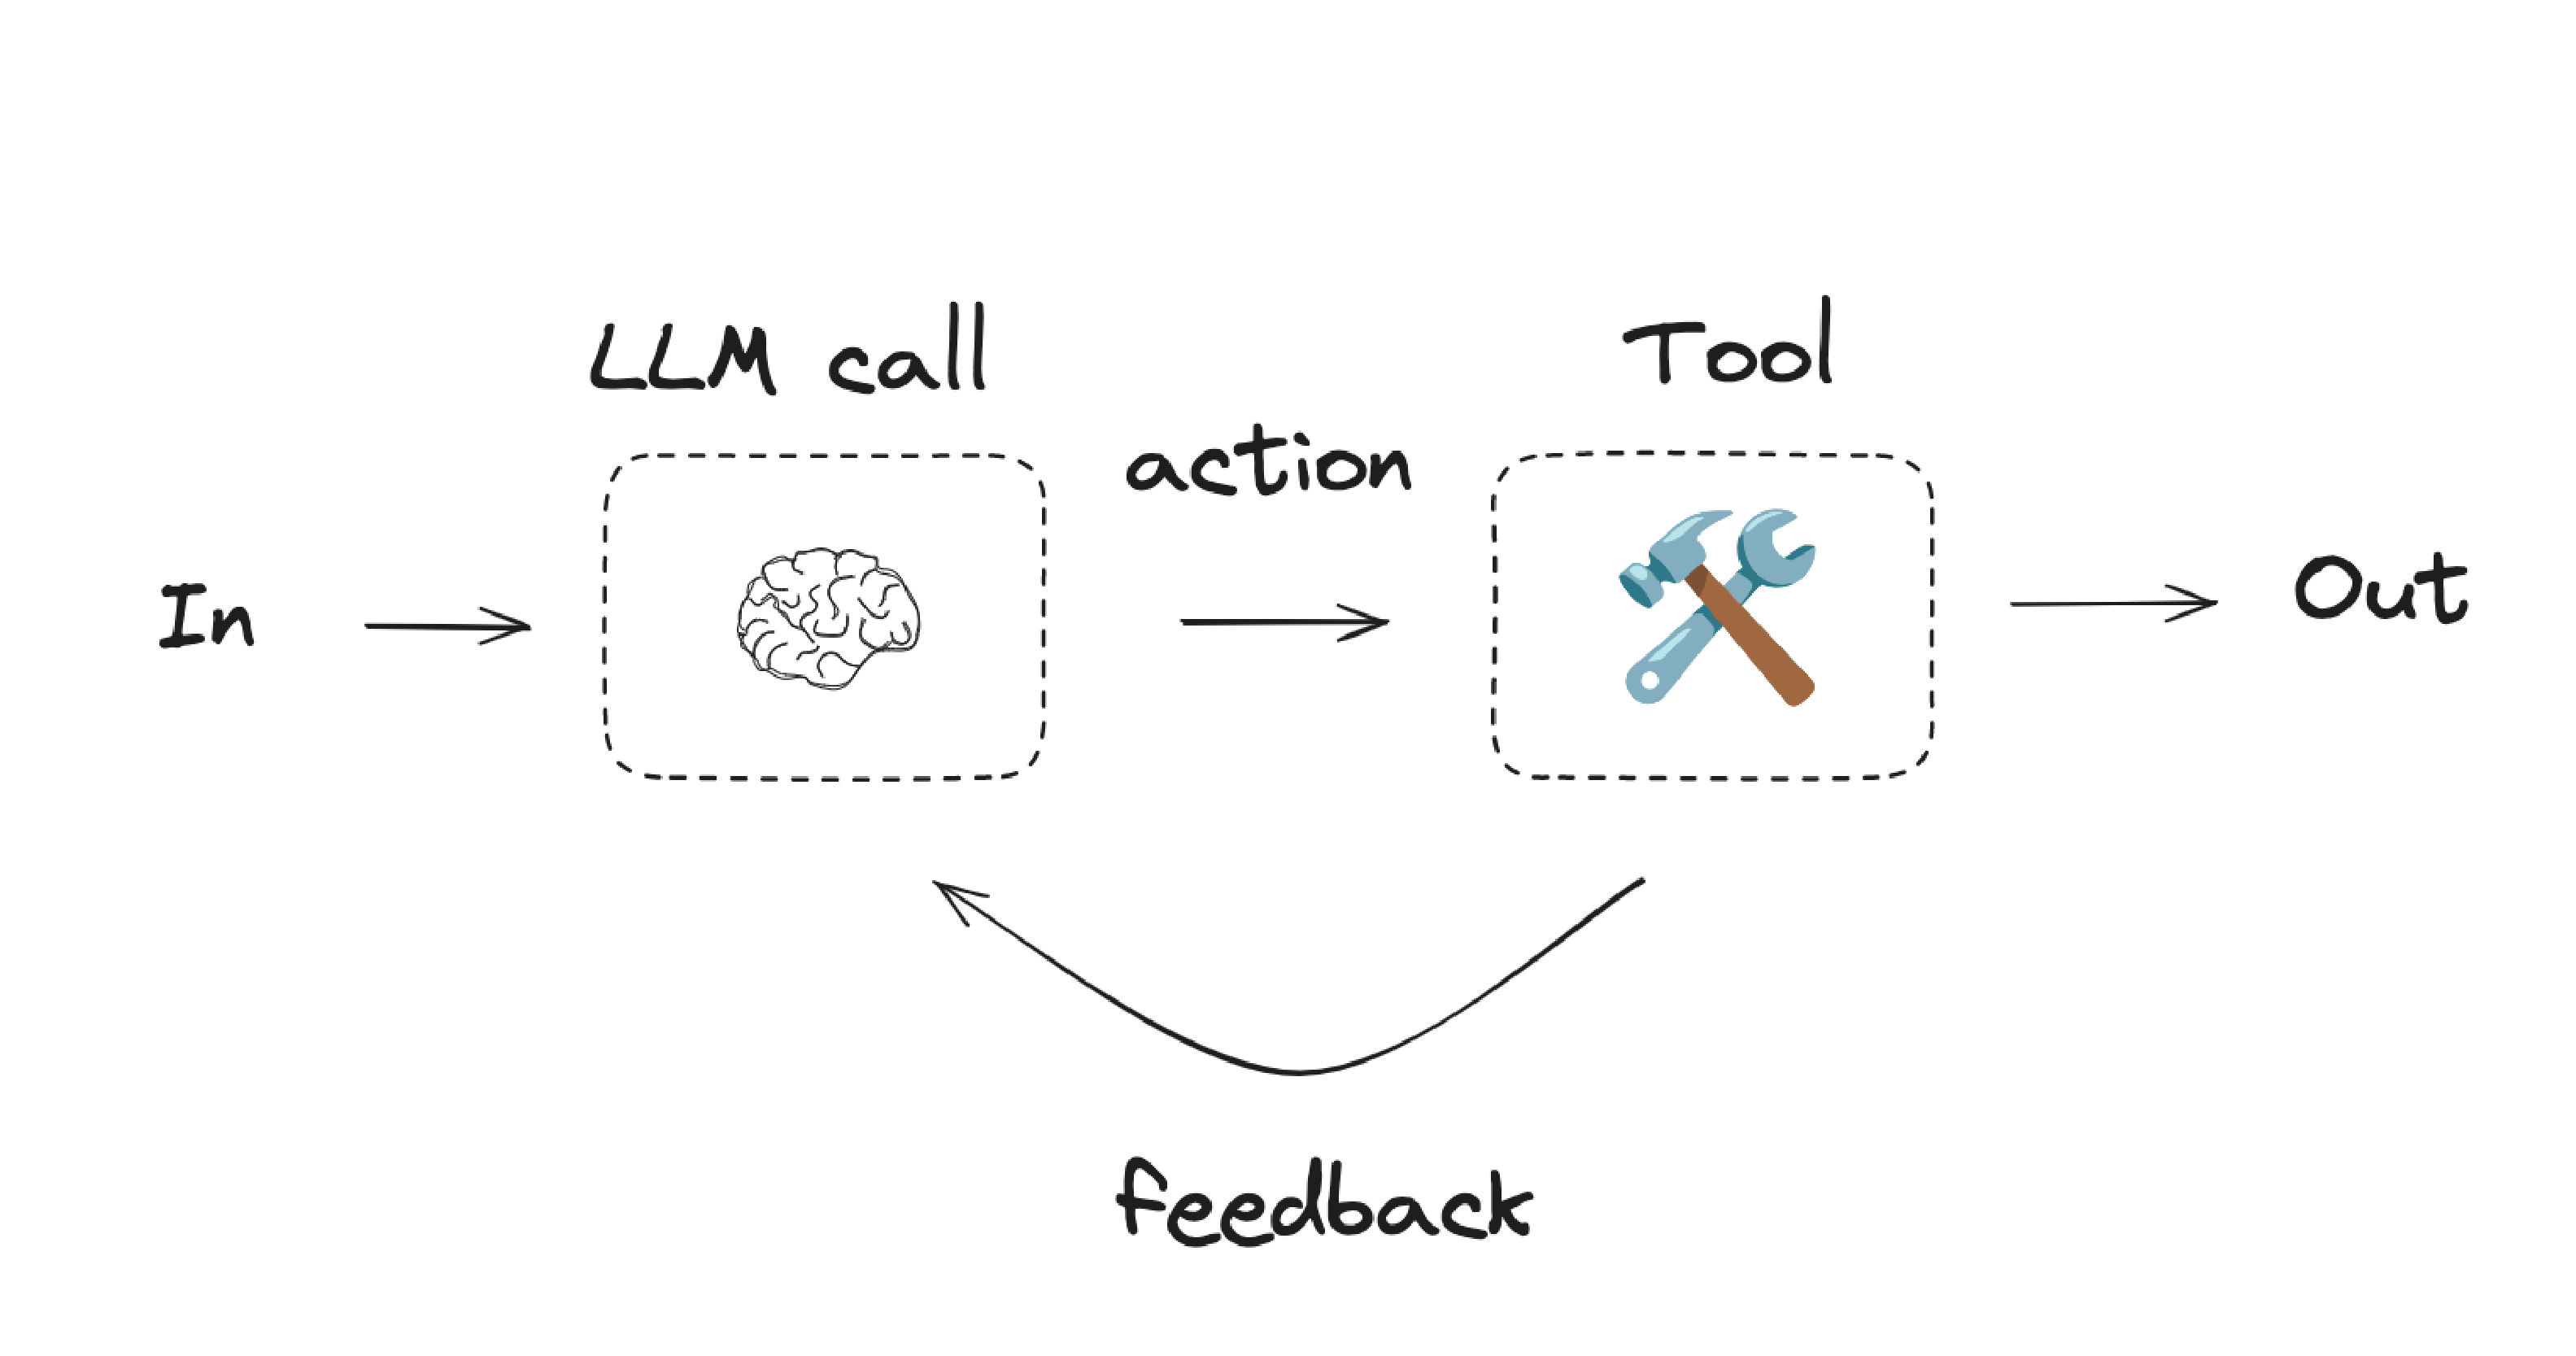
\includegraphics[width=\linewidth,height=3.7cm,keepaspectratio]{images/real_framework_langgraph_workflow_agent.pdf}
\par{\fontsize{7}{8.3}\selectfont\color{Slate} Original LangGraph documentation figure. The model chooses an action, receives feedback and can choose again.}
\par\endgroup\smallskip
{
\small\begin{itemize}
\setlength{\itemsep}{.25em}
\item In a fixed workflow, code sets the steps and branches.
\item In an LLM agent, the model chooses some next steps from the allowed actions, using the results so far.
\end{itemize}\par}
\vfill
{\fontsize{6.3}{7.5}\selectfont\color{Slate} Source: \href{https://www.anthropic.com/engineering/building-effective-agents}{Erik S., Barry Zhang. Building effective agents. Anthropic Engineering. 2024-12-19.}\par}
\note{This distinction comes from Anthropic's practitioner account. It is useful engineering language, not a universal definition. Its workflow patterns include routing, orchestrator-workers and evaluator-optimizer loops. A system can combine fixed requirements with an LLM choosing among allowed next steps. PowerDAG later shows this combination. Source: LangChain documentation maintainers, official LangGraph documentation. Accessed October 18, 2026. This documentation convention concerns LLM applications, not all classical AI agents. Source figure locator: Opening workflow comparison: selected Agent panel. Original source URL: https://docs.langchain.com/oss/python/langgraph/workflows-agents Takeaway: 

Erik S., Barry Zhang. Building effective agents. Anthropic Engineering. 2024-12-19.
Full source: https://www.anthropic.com/engineering/building-effective-agents

LangChain maintainers. LangGraph overview. Docs by LangChain, Python open-source documentation. Undated live documentation; accessed 2026-10-17.
Full source: https://docs.langchain.com/oss/python/langgraph/overview

LangChain documentation maintainers. Workflows and agents. Docs by LangChain, Python LangGraph documentation. Undated live documentation; accessed October 18, 2026.
Full source: https://docs.langchain.com/oss/python/langgraph/workflows-agents}
\end{frame}

\begin{frame}[t]{An agent needs a clear goal and limits}
\relax
\begin{columns}[T,onlytextwidth]\begin{column}{.64\textwidth}
\begingroup\centering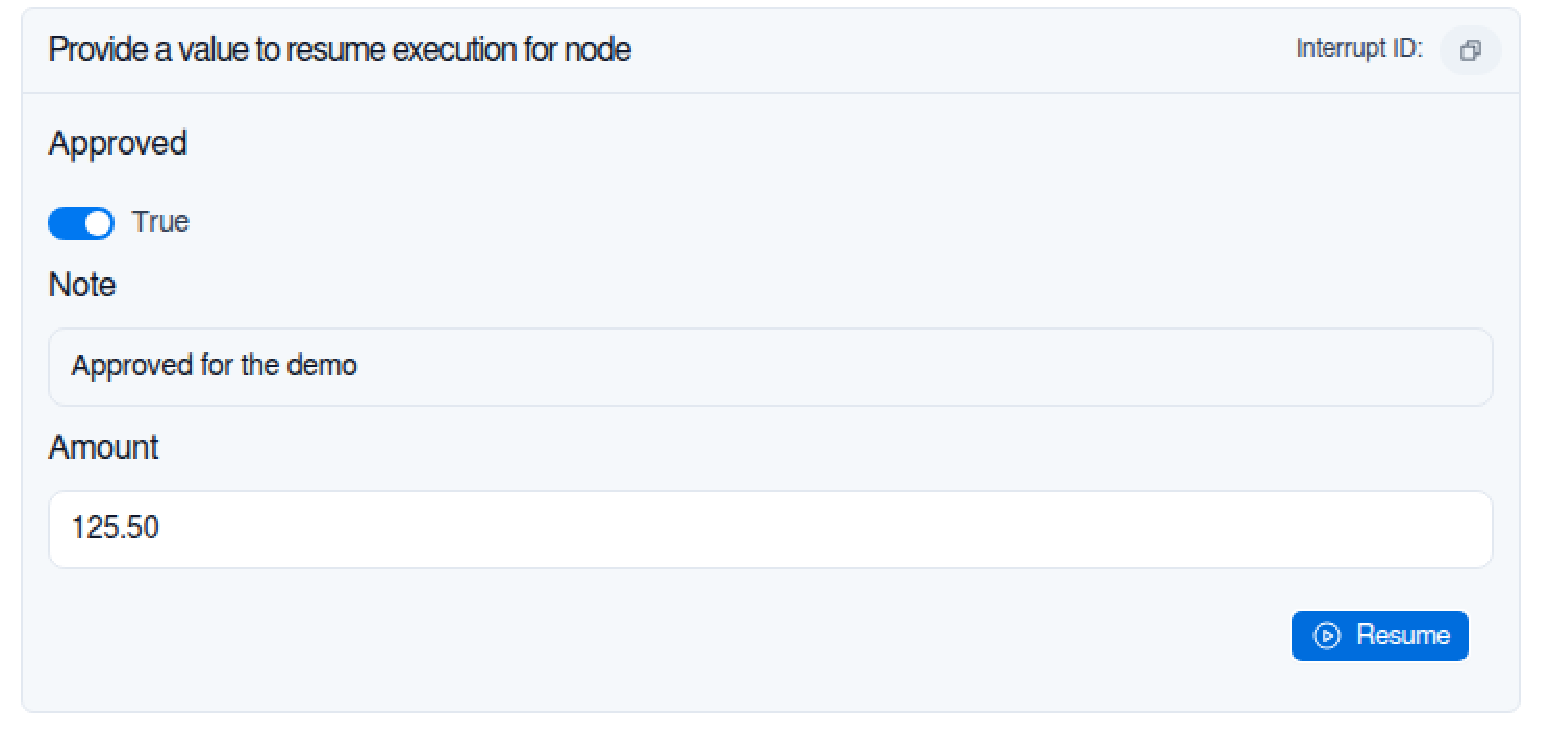
\includegraphics[width=\linewidth,height=4.65cm,keepaspectratio]{images/real_framework_langgraph_review_detail.pdf}
\par{\fontsize{7}{8.3}\selectfont\color{Slate} Original LangGraph Studio review-form excerpt. This is a generic demo, not a utility interface.}
\par\endgroup\smallskip
\end{column}\begin{column}{.32\textwidth}
{
\small\begin{itemize}
\setlength{\itemsep}{.25em}
\item The agent can run agreed studies and prepare a report with evidence.
\item The operator reviews the findings and decides whether an operating action is allowed.
\end{itemize}\par}
\end{column}\end{columns}
\vfill
{\fontsize{6.3}{7.5}\selectfont\color{Slate} Source: \href{https://docs.langchain.com/oss/python/langgraph/interrupts}{LangChain documentation maintainers. LangGraph Interrupts. Official LangChain documentation. Accessed 2026-10-17; live documentation.}\par}
\note{This is an illustrative advisory-study policy informed by classical work on agency. Wooldridge and Jennings discuss autonomy, response to change, initiative and interaction; they do not prescribe this grid-operator approval process. The example gives the agent permission to run agreed studies and prepare evidence. The operator can request changes, stop the process or approve a later operating action. This diagram does not give the agent direct control of physical equipment. Source: LangChain documentation maintainers, official LangGraph documentation. Accessed October 18, 2026. This is a generic software demonstration, not an operator dispatch interface or a utility deployment. Source figure locator: Interrupt response schema / Studio form. Original source URL: https://docs.langchain.com/oss/python/langgraph/interrupts Takeaway: 

Michael Wooldridge, Nicholas R. Jennings. Intelligent agents: theory and practice. The Knowledge Engineering Review, 10(2), pp. 115--152. 1995.
Full source: https://doi.org/10.1017/S0269888900008122
Full paper: https://www.cs.ox.ac.uk/people/michael.wooldridge/pubs/ker95.pdf

Stuart J. Russell, Peter Norvig. Artificial Intelligence: A Modern Approach, Chapter 2: Intelligent Agents. Prentice Hall, second edition, Chapter 2, pp. 32--58. 2003.
Full source: https://aima.cs.berkeley.edu/2nd-ed/
Full paper: https://aima.cs.berkeley.edu/4th-ed/pdfs/newchap02.pdf

LangChain documentation maintainers. LangGraph Interrupts. Official LangChain documentation. Accessed 2026-10-17; live documentation.
Full source: https://docs.langchain.com/oss/python/langgraph/interrupts}
\end{frame}

\begin{frame}[t]{A model can use records, tools and memory}
\relax
\begingroup\centering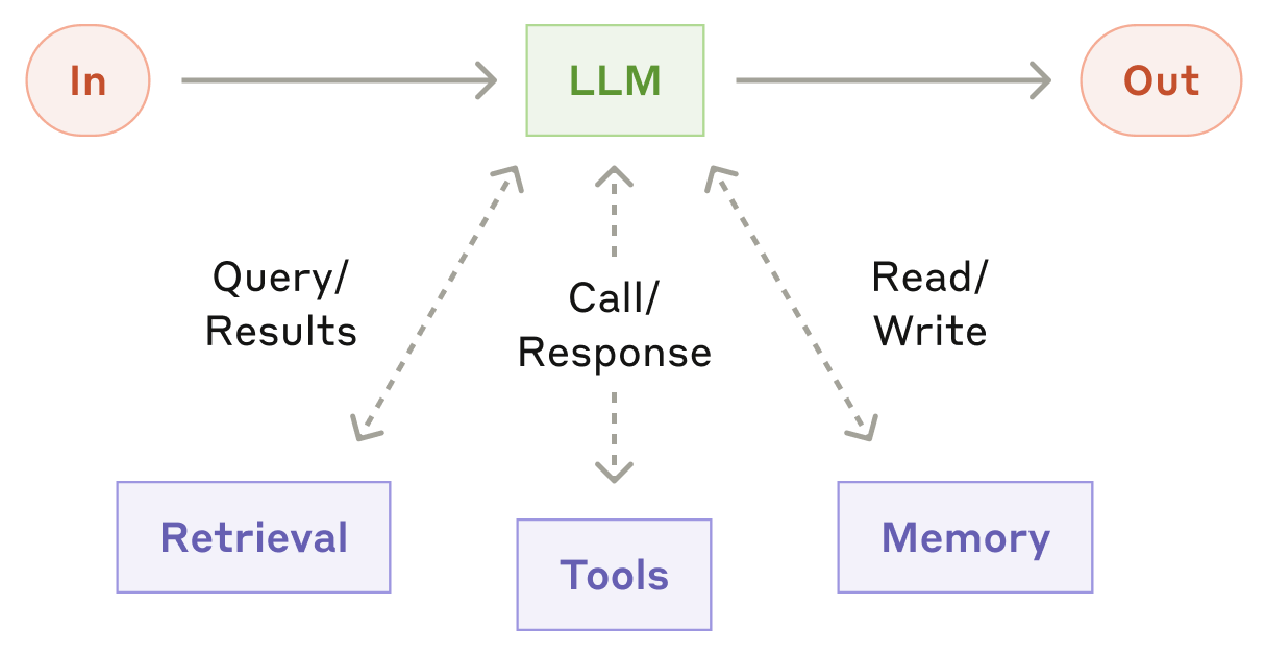
\includegraphics[width=\linewidth,height=3.95cm,keepaspectratio]{images/source_anthropic_augmented_llm_wide.pdf}
\par{\fontsize{7}{8.3}\selectfont\color{Slate} Original Anthropic building-block figure. It is a general pattern, not a diagram of PowerAgent or PowerDAG.}
\par\endgroup\smallskip
{
\small\begin{itemize}
\setlength{\itemsep}{.25em}
\item Retrieval finds records; tools run tasks; memory keeps useful context.
\item LangGraph can manage the steps. PowerAgent supplies power-domain components; PowerDAG is one specific system.
\end{itemize}\par}
\vfill
{\fontsize{6.3}{7.5}\selectfont\color{Slate} Source: \href{https://www.anthropic.com/engineering/building-effective-agents}{Erik S., Barry Zhang. Building effective agents. Anthropic Engineering. 2024-12-19.}\par}
\note{These names refer to different roles. LangGraph can run both fixed workflows and processes where a model chooses steps. PowerAgent develops power-system models, tool interfaces and workflows. Later slides show a specific LangGraph example in its PowerWF repository. PowerDAG has its own supervisory design. A platform name alone does not establish numerical accuracy or deployment at a utility. The published figure shows an augmented language model. Retrieval, tools and memory are supporting capabilities; they are not mandatory in every agent. The diagram is reproduced from Anthropic with only empty margins trimmed in the display. The original image bytes are retained. Takeaway: 

Erik S., Barry Zhang. Building effective agents. Anthropic Engineering. 2024-12-19.
Full source: https://www.anthropic.com/engineering/building-effective-agents

LangChain maintainers. LangGraph overview. Docs by LangChain, Python open-source documentation. Undated live documentation; accessed 2026-10-17.
Full source: https://docs.langchain.com/oss/python/langgraph/overview

Power and AI Initiative / PowerAgent community, Harvard SEAS. PowerAgent --- Open-Source Agentic AI for Power Grids. Official Harvard project website. Live project page reviewed 17 October 2026.
Full source: https://poweragent.seas.harvard.edu/

Emmanuel O. Badmus, Amritanshu Pandey. PowerDAG: Supervisory Agentic AI System for Automating Distribution Grid Analysis. arXiv preprint, version 4. 5 July 2026 (v4); first submitted 18 March 2026.
Full source: https://arxiv.org/pdf/2603.17418v4}
\end{frame}

\begin{frame}[t]{PJM uses HyperQ to review connection applications}
\relax
{\scriptsize\color{Slate}\textbf{United States / Supplier reports deployment / PJM confirms earlier testing}\par}\smallskip
\begin{columns}[T,onlytextwidth]\begin{column}{.515\textwidth}
{
\normalsize\begin{itemize}
\item Tapestry's June 2026 report says HyperQ entered PJM Cycle 1 on 29 April. PJM confirmed testing in March.
\item Gemini agents check site-control agreements (rights to use land), property parcels and tariff evidence. Engineers make final decisions.
\item This work checks application readiness before the electrical study begins.
\end{itemize}\par}
\end{column}\begin{column}{.445\textwidth}
\begingroup\centering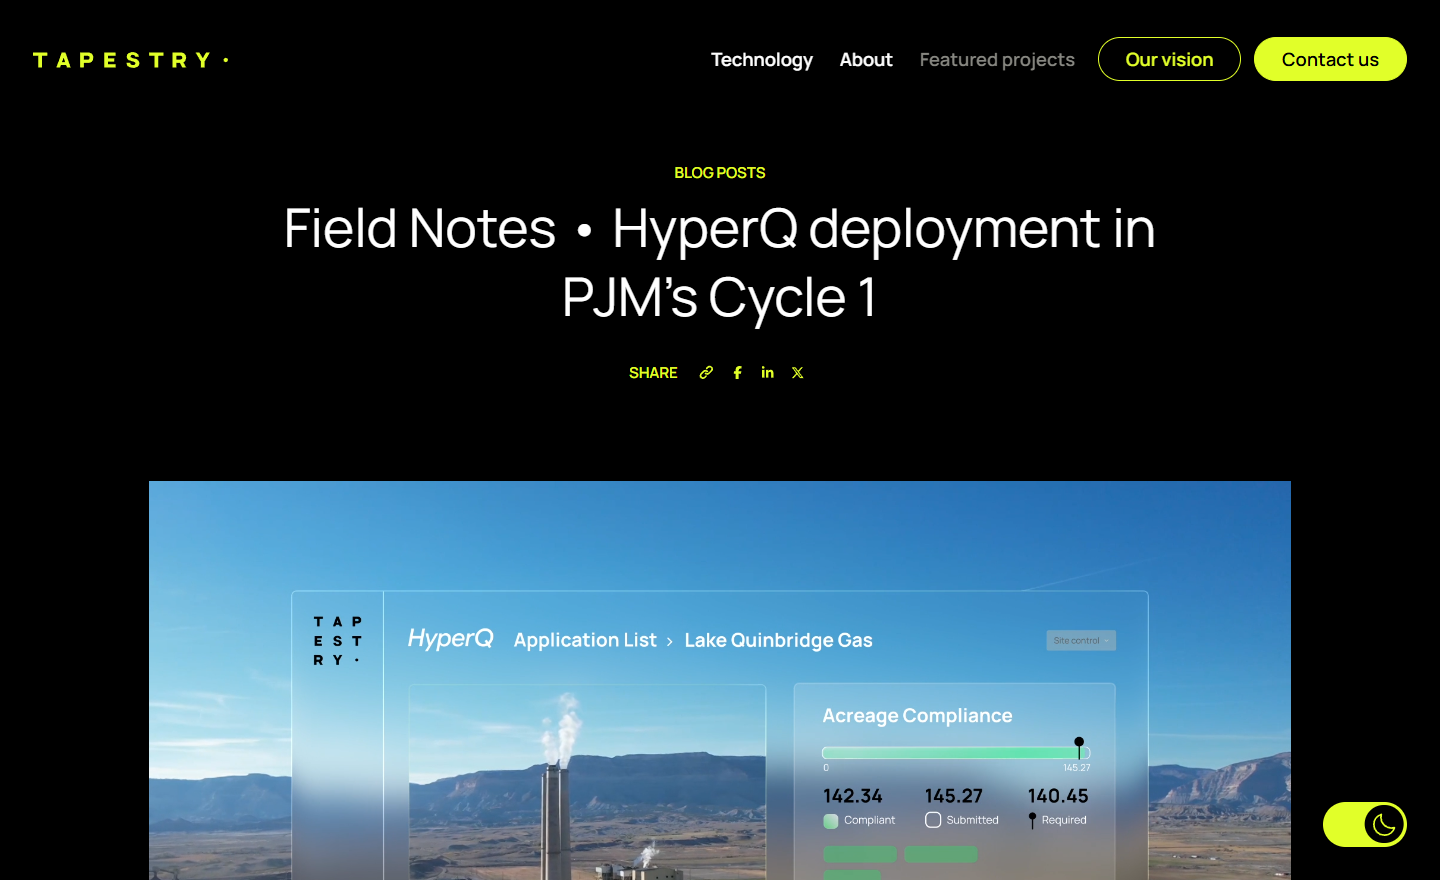
\includegraphics[width=\linewidth,height=3.7cm,keepaspectratio]{images/real_news_pjm_hyperq_header.png}
\par{\fontsize{7}{8.3}\selectfont\color{Slate} Original Tapestry article and published animation still. Supplier report, June 2026.}
\par\endgroup\smallskip
\end{column}\end{columns}
\vfill
{\small\color{IEEEBlue}\textbf{A numerical study needs reliable input evidence.}\par}\smallskip
{\fontsize{6.3}{7.5}\selectfont\color{Slate} Source: \href{https://www.tapestryenergy.com/en/projects/field-notes-hyperq-deployment-in-pjm-s-cycle-1}{Tapestry. Field Notes  /  HyperQ deployment in PJM's Cycle 1. 2026-06-11; deployment entry 2026-04-29.}\par}
\note{Tapestry's 11 June report covers 811 generation applications. Agents perform limited document and evidence tasks. The report does not establish an agent making a power-flow conclusion or an automatic regulatory decision. The system guides the agents' work and records evidence citations. The article describes migration to Google ADK as future work, so do not label the deployed system an established ADK implementation. Tapestry, HyperQ Field Notes, June 11, 2026 Supplier report of deployment. PJM separately confirmed earlier testing. The hero is a still captured from the publisher's animation, not an independently verified live PJM application record. Original page: https://www.tapestryenergy.com/en/projects/field-notes-hyperq-deployment-in-pjm-s-cycle-1 Takeaway: A numerical study needs reliable input evidence.

Tapestry. Field Notes  /  HyperQ deployment in PJM's Cycle 1. 2026-06-11; deployment entry 2026-04-29.
Full source: https://www.tapestryenergy.com/en/projects/field-notes-hyperq-deployment-in-pjm-s-cycle-1

Tapestry. How agentic AI can help grid operators speed up interconnection. 2025.
Full source: https://www.tapestryenergy.com/en/projects/how-agentic-ai-can-help-grid-operators-speed-up-interconnection

PJM Interconnection. Successful Interconnection Reforms, Other PJM Initiatives Seek To Maximize Electricity Supplies. 2026-03-16.
Full source: https://insidelines.pjm.com/connected/}
\end{frame}

\begin{frame}[t]{HyperQ: what the reported numbers measure}
\relax
\begingroup\centering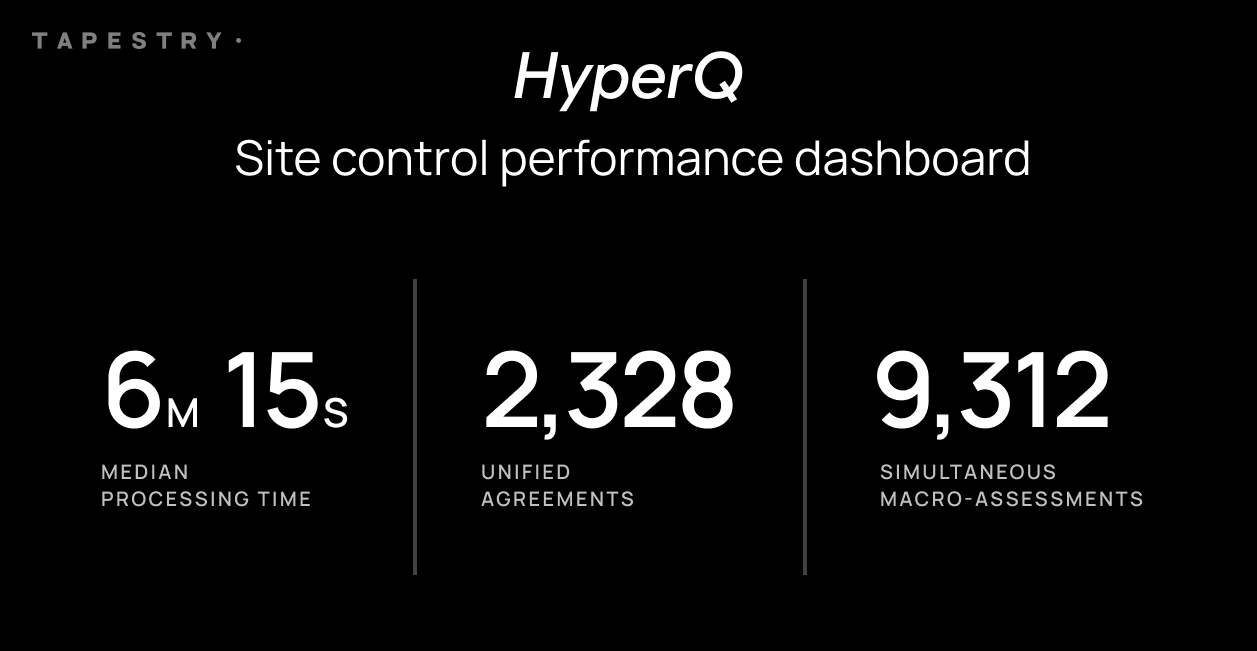
\includegraphics[width=\linewidth,height=3.65cm,keepaspectratio]{images/power_news_hyperq_dashboard.png}
\par{\fontsize{7}{8.3}\selectfont\color{Slate} Original Tapestry performance graphic, June 2026. The timing covers only computer processing.}
\par\endgroup\smallskip
{
\small\begin{itemize}
\setlength{\itemsep}{.25em}
\item The timings cover computer processing for 811 applications. They exclude document-transfer time and human validation.
\end{itemize}\par}
\vfill
{\fontsize{6.3}{7.5}\selectfont\color{Slate} Source: \href{https://www.tapestryenergy.com/en/projects/field-notes-hyperq-deployment-in-pjm-s-cycle-1}{Tapestry. Field Notes  /  HyperQ deployment in PJM's Cycle 1. 2026-06-11; deployment entry 2026-04-29.}\par}
\note{The supplier reports grouping 4,581 raw site-control documents into 2,328 bundles and checking four criteria. The graphic's 9,312 macro-assessments are not 9,312 projects. The full interconnection process also includes document transfer and human review. The report gives no confusion matrix or accuracy denominator. We omit its historical 20x headline because it compares manual work with computer processing using different work and timing boundaries. Takeaway: 

Tapestry. Field Notes  /  HyperQ deployment in PJM's Cycle 1. 2026-06-11; deployment entry 2026-04-29.
Full source: https://www.tapestryenergy.com/en/projects/field-notes-hyperq-deployment-in-pjm-s-cycle-1}
\end{frame}

\begin{frame}[t]{CAISO/OATI: agents help review planned outages}
\relax
\begin{columns}[T,onlytextwidth]\begin{column}{.515\textwidth}
{
\normalsize\begin{itemize}
\item OATI's AI Genie uses Workflow, Advisor and Recon agents under one coordinator. Operators keep final authority.
\item The supplier reports processing 500+ next-day requests nightly in under eight minutes. It gives no per-request time or reviewer-effort result.
\end{itemize}\par}
\end{column}\begin{column}{.445\textwidth}
\begingroup\centering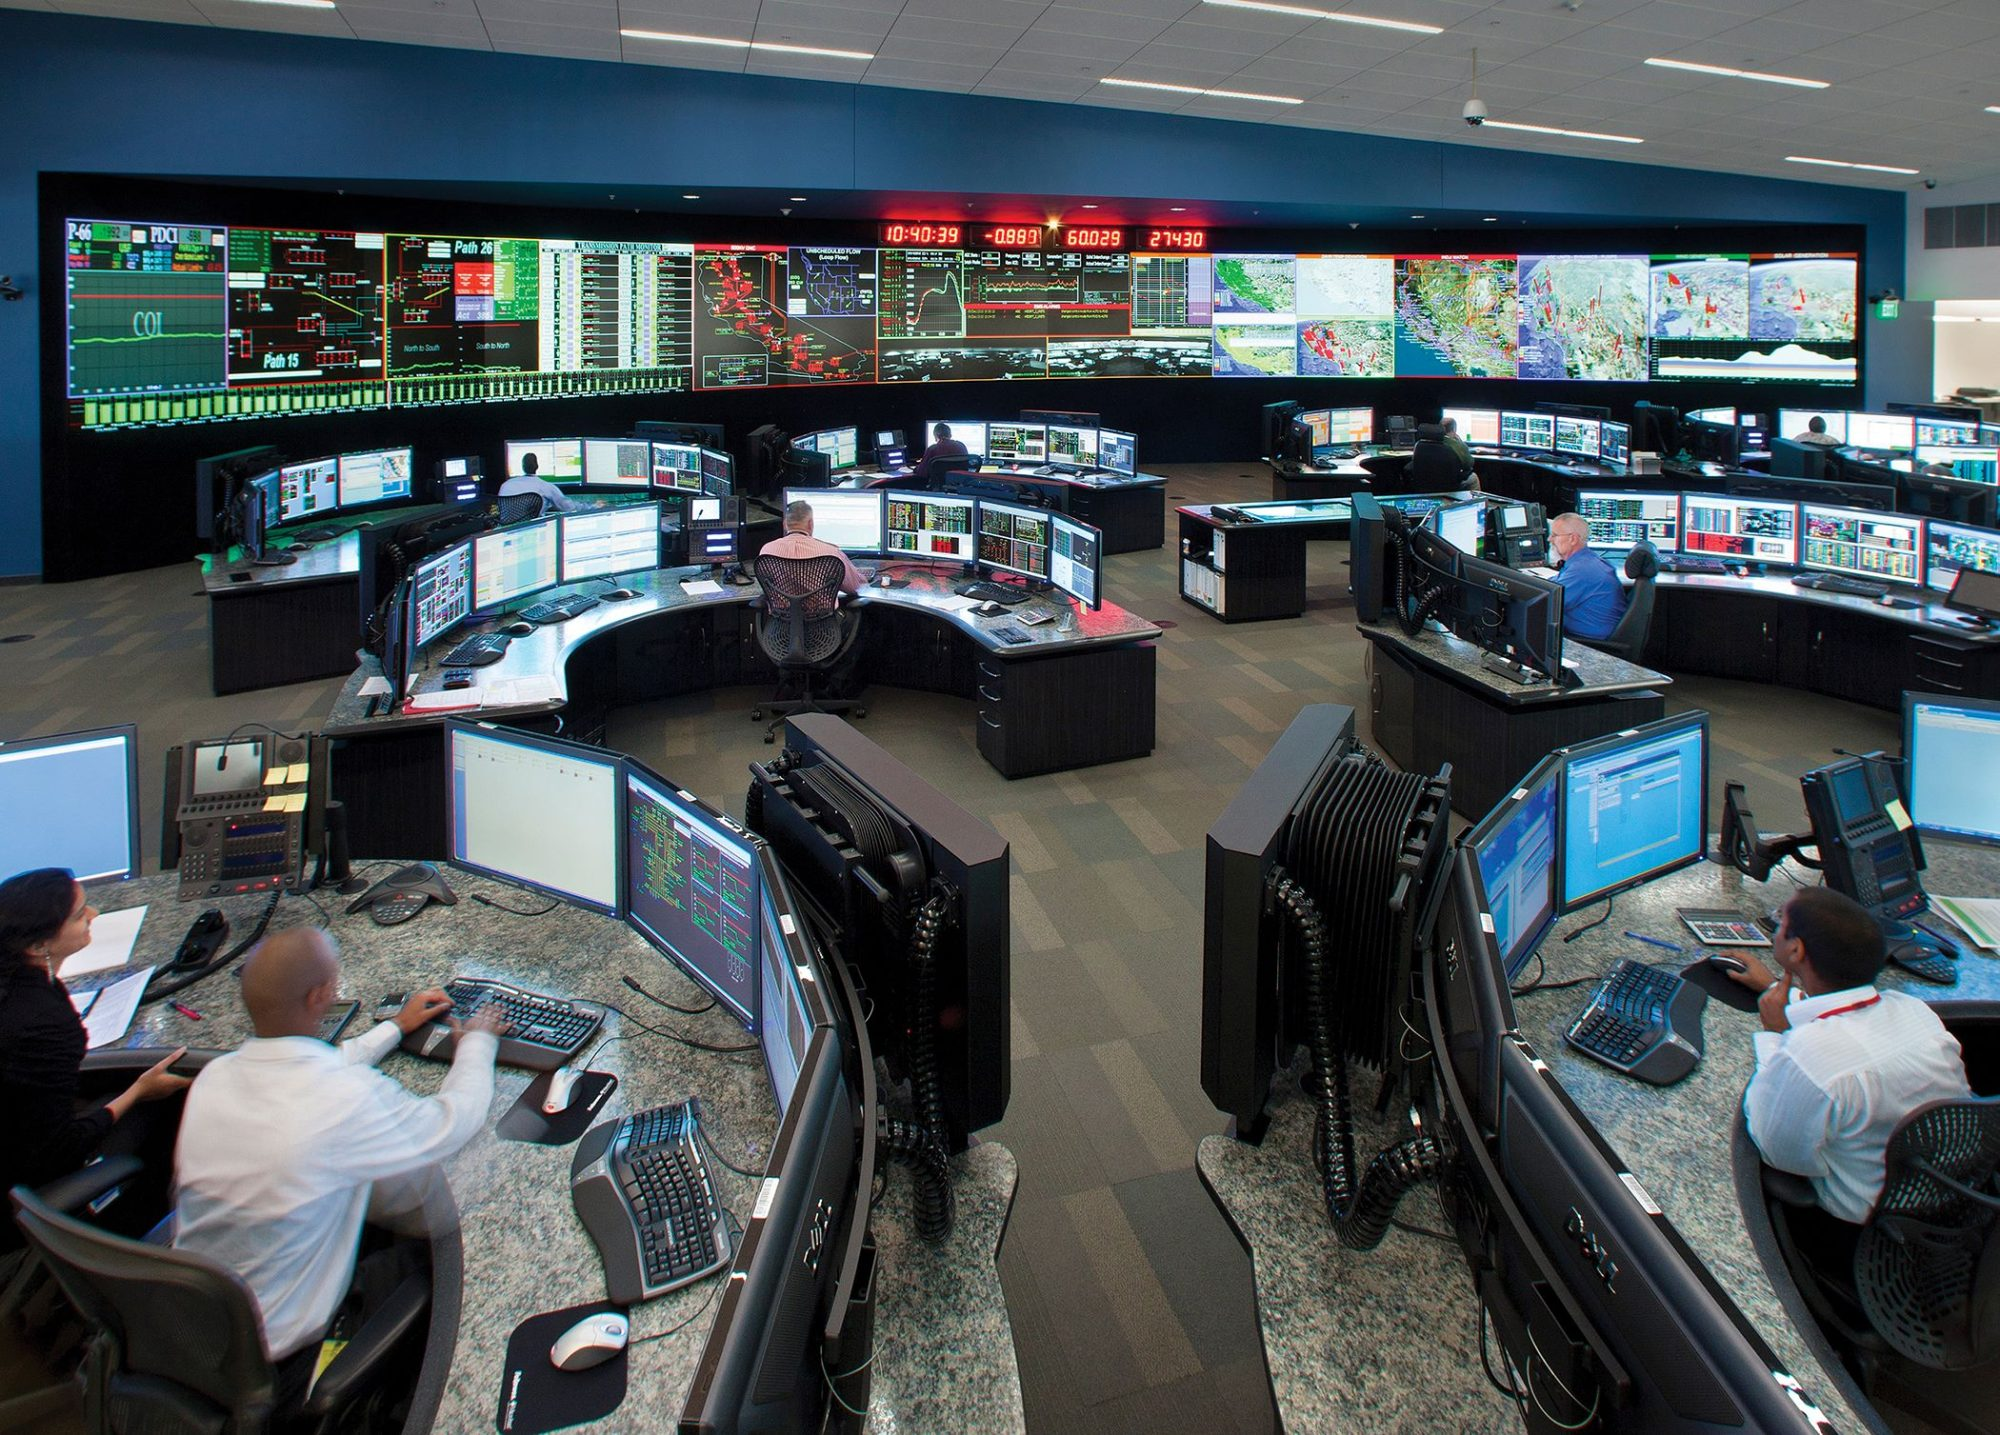
\includegraphics[width=\linewidth,height=3.85cm,keepaspectratio]{images/caiso_control_room.jpg}
\par{\fontsize{7}{8.3}\selectfont\color{Slate} Real California ISO control room. OATI supplies the batch result and later production-use claim.}
\par\endgroup\smallskip
\end{column}\end{columns}
\vfill
{\small\color{IEEEBlue}\textbf{A processing rate needs a clear work boundary and a measure of the review left for people.}\par}\smallskip
{\fontsize{6.3}{7.5}\selectfont\color{Slate} Source: \href{https://www.oati.com/ai-for-energy/}{OATI. Generative and Agentic AI in Grid Operations: Field Lessons from OATI, CAISO, PNNL, and EPRI. 2026 (exact publication day not displayed).}\par}
\note{California ISO's July 2025 account described a pilot. OATI's 2026 field report describes daily production use but gives no exact production start date. The reported inequalities imply more than 62.5 requests per minute for the batch. They do not describe individual request latency. Do not compare eight machine-minutes with a separate analyst-hours figure as though both came from the same trial. The work prepares outage analysis and operating evidence. Reviewers make final decisions. Takeaway: A processing rate needs a clear work boundary and a measure of the review left for people.

California ISO. Exploring AI to support smarter grid management. 2025-07-28.
Full source: https://www.caiso.com/about/news/energy-matters-blog/exploring-ai-to-support-smarter-grid-management

OATI. Generative and Agentic AI in Grid Operations: Field Lessons from OATI, CAISO, PNNL, and EPRI. 2026 (exact publication day not displayed).
Full source: https://www.oati.com/ai-for-energy/

OATI (California ISO control-room photograph). California ISO control room, image published by OATI: California ISO control room with operators seated at curved desks facing a long wall of grid displays. Image accessed 17 October 2026.
Full source: https://www.oati.com/ai-genie/}
\end{frame}

\begin{frame}[t]{Duke and AWS: agents help prepare planning studies}
\relax
\begin{columns}[T,onlytextwidth]\begin{column}{.515\textwidth}
{
\normalsize\begin{itemize}
\item Duke engineers use AWS-managed agents to prepare study cases and coordinate interconnection studies for new grid connections.
\item A September 2026 AWS announcement reports data preparation falling from two weeks of manual work to hours.
\item The final number of hours is unspecified. Engineers keep final responsibility for engineering decisions.
\end{itemize}\par}
\end{column}\begin{column}{.445\textwidth}
\begingroup\centering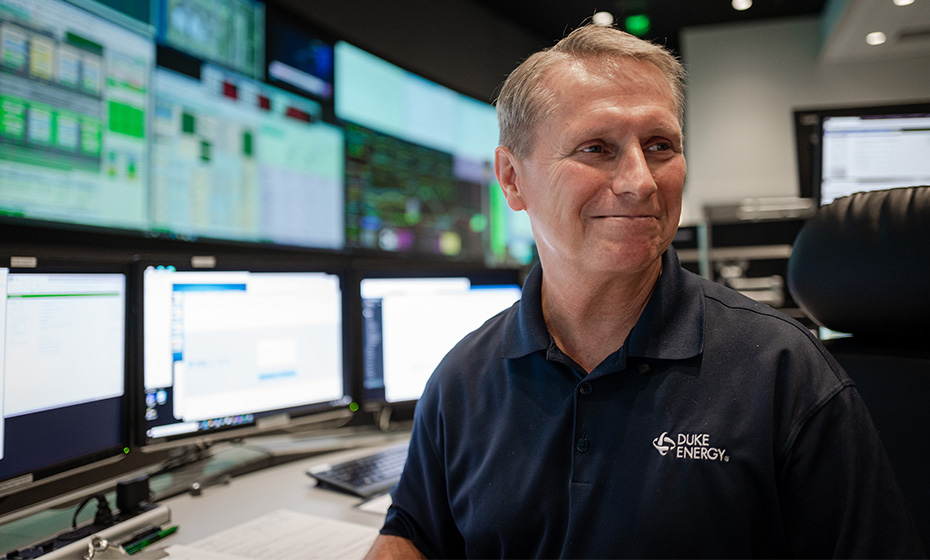
\includegraphics[width=\linewidth,height=3.85cm,keepaspectratio]{images/duke_operator.jpg}
\par{\fontsize{7}{8.3}\selectfont\color{Slate} Duke operator, 2022, shown for context. The reported agents support planning, rather than this pictured operating desk.}
\par\endgroup\smallskip
\end{column}\end{columns}
\vfill
{\small\color{IEEEBlue}\textbf{Faster preparation alone does not establish a shorter full regulatory process.}\par}\smallskip
{\fontsize{6.3}{7.5}\selectfont\color{Slate} Source: \href{https://press.aboutamazon.com/aws/2026/9/aws-launches-agentic-grid-planning-program-to-accelerate-interconnection-studies}{Amazon Web Services. AWS Launches Agentic Grid Planning Program to Accelerate Interconnection Studies. 2026-09-17.}\par}
\note{AWS's 17 September 2026 announcement names Duke engineers using agents to coordinate studies. The agents prepare inputs and coordinate existing physics software, models and scripts. The report says data preparation fell from two weeks of manual work to hours. It gives neither the final number of hours nor a sample count. It identifies no SDK, model or runtime. Do not infer Strands or AgentCore from the cloud provider. Engineers make final decisions. Takeaway: Faster preparation alone does not establish a shorter full regulatory process.

Amazon Web Services. AWS Launches Agentic Grid Planning Program to Accelerate Interconnection Studies. 2026-09-17.
Full source: https://press.aboutamazon.com/aws/2026/9/aws-launches-agentic-grid-planning-program-to-accelerate-interconnection-studies

Amazon Web Services. Agentic Grid Planning on AWS. Undated; reviewed 17 October 2026.
Full source: https://aws.amazon.com/energy-utilities/agentic-grid-planning/

Duke Energy / illumination. Duke Energy, illumination, August 2, 2022: Duke Energy grid operator Howard Greene seated before many control-room displays. Image accessed 17 October 2026.
Full source: https://illumination.duke-energy.com/articles/meet-the-team-that-monitors-the-grid-and-keeps-the-lights-on}
\end{frame}

\begin{frame}[t]{Siemens announces agents for PSS E planning studies}
\relax
{\scriptsize\color{Slate}\textbf{Product announcement / 5 May 2026}\par}\smallskip
\begin{columns}[T,onlytextwidth]\begin{column}{.515\textwidth}
{
\normalsize\begin{itemize}
\item Siemens' Gridscale X announcement describes agents coordinating transmission-planning simulations.
\item The targets include connection studies for large loads and data centers, using open software interfaces (APIs).
\item The announcement does not name a production user of the new agentic PSS E features.
\end{itemize}\par}
\end{column}\begin{column}{.445\textwidth}
\begingroup\centering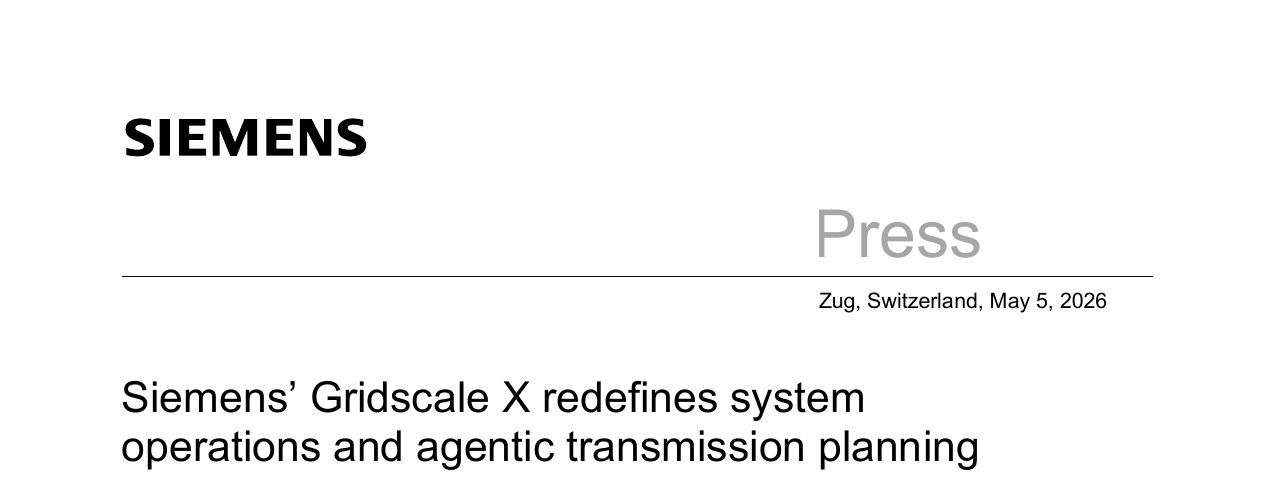
\includegraphics[width=\linewidth,height=3.85cm,keepaspectratio]{images/real_news_siemens_gridscale_header.png}
\par{\fontsize{7}{8.3}\selectfont\color{Slate} Original Siemens press-release header, 2026. This is an announced product capability.}
\par\endgroup\smallskip
\end{column}\end{columns}
\vfill
{\small\color{IEEEBlue}\textbf{Check product features and measured utility results separately.}\par}\smallskip
{\fontsize{6.3}{7.5}\selectfont\color{Slate} Source: \href{https://press.siemens.com/global/en/pressrelease/siemens-gridscale-x-redefines-system-operations-and-agentic-transmission-planning}{Siemens. Siemens' Gridscale X redefines system operations and agentic transmission planning. 2026-05-05.}\par}
\note{The same release describes Alliander's migration to the platform. That shows platform adoption, not use of the newly announced agentic PSS E features. The claim of up to 50\% faster study response has no disclosed benchmark method, so we do not plot it. The announcement shows a possible integration path: agents coordinate an established simulation environment. Siemens AG, press release, May 5, 2026 Product announcement. The separately named Alliander platform migration does not prove production use of the new agentic PSS E capability. Original page: https://press.siemens.com/global/en/pressrelease/siemens-gridscale-x-redefines-system-operations-and-agentic-transmission-planning Takeaway: Check product features and measured utility results separately.

Siemens. Siemens' Gridscale X redefines system operations and agentic transmission planning. 2026-05-05.
Full source: https://press.siemens.com/global/en/pressrelease/siemens-gridscale-x-redefines-system-operations-and-agentic-transmission-planning}
\end{frame}

\begin{frame}[t]{National Grid reports agents checking project plans}
\relax
{\scriptsize\color{Slate}\textbf{Reported current use / UK--US group / Rollout location unspecified}\par}\smallskip
{
\normalsize\begin{itemize}
\item The results transcript says its "capital control tower" already checks early project options and documents at approval stages.
\item Project managers get feedback while they can still change their plans.
\item The group reports no agent framework, timing result or accuracy result.
\end{itemize}\par}
\vfill
{\fontsize{6.3}{7.5}\selectfont\color{Slate} Source: \href{https://www.nationalgrid.com/document/577036/download}{National Grid. National Grid Full Year Results 2025/26: Video Webcast Transcript. 2026-05-14.}\par}
\note{The CEO's 14 May 2026 results transcript reports agentic project-assurance use. "Capital control tower" names the system supporting project checks. Later comments about optimizing access outages describe future plans. Do not attribute nearby FLISR, outage-minute or gas-crew results to this agent. The source verifies reported use without supporting a numerical performance estimate. Takeaway: 

National Grid. National Grid Full Year Results 2025/26: Video Webcast Transcript. 2026-05-14.
Full source: https://www.nationalgrid.com/document/577036/download}
\end{frame}

\begin{frame}[t]{NYPA: better data for agent use}
\relax
{\scriptsize\color{Slate}\textbf{NYPA data-quality lead / Webinar, 14 October 2026}\par}\smallskip
\begin{columns}[T,onlytextwidth]\begin{column}{.64\textwidth}
\begingroup\centering
\includegraphics[width=\linewidth,height=4.4cm,keepaspectratio]{images/real_news_nypa_webinar_detail.pdf}
\par{\fontsize{7}{8.3}\selectfont\color{Slate} Original Ataccama webinar artwork. The NYPA speaker appears at lower right.}
\par\endgroup\smallskip
\end{column}\begin{column}{.32\textwidth}
{
\small\begin{itemize}
\setlength{\itemsep}{.25em}
\item NYPA describes Databricks and Ataccama checks for meter data before AI uses it.
\item A separate demo connects Genie to Ataccama through the Model Context Protocol (MCP). Its product-data example does not establish NYPA grid control.
\end{itemize}\par}
\end{column}\end{columns}
\vfill
{\fontsize{6.3}{7.5}\selectfont\color{Slate} Source: \href{https://www.ataccama.com/webinar/on-demand-trust-driven-medallion-architecture}{Session speakers: Saptaparna Gupta (NYPA), Oleksandra Bovkun (Databricks), Eliza Pochinova (Ataccama). On demand: Trust-driven medallion architecture: How to make your CDEs ready for AI. Ataccama. 2026.}\par}
\note{This supplier-hosted webinar discusses NYPA's quality checks for frequently arriving meter data. The separate demo uses Genie and an Ataccama MCP service with a product/reorder table. MCP, the Model Context Protocol, is a standard way to connect AI systems to tools and data. Keep the NYPA implementation and the generic agent demo separate. We use October 2026 because the fetched event and on-demand report show adjacent dates. These sources support the discussion of data agents need, without establishing a production grid-command agent at NYPA. We excluded the earlier governance-agenda search result because the full original was unavailable. Ataccama, original webinar report with NYPA Data Quality Lead Saptaparna Gupta, October 14, 2026 NYPA discusses meter-data quality checks. The separate product/reorder demo does not establish a production NYPA grid-control agent. Original page: https://www.ataccama.com/webinar/on-demand-trust-driven-medallion-architecture Takeaway: 

Session speakers: Saptaparna Gupta (NYPA), Oleksandra Bovkun (Databricks), Eliza Pochinova (Ataccama). On demand: Trust-driven medallion architecture: How to make your CDEs ready for AI. Ataccama. 2026.
Full source: https://www.ataccama.com/webinar/on-demand-trust-driven-medallion-architecture

Saptaparna Gupta (NYPA), Oleksandra Bovkun (Databricks), Eliza Pochinova (Ataccama). Trust-driven medallion architecture: how to make your CDEs ready for AI. Ataccama. 2026-10-13, 11:00 AM EDT (date displayed on fetched event page).
Full source: https://www.ataccama.com/events/trust-driven-medallion-architecture}
\end{frame}

\begin{frame}[t]{Eversource: adding agentic skills to grid studies}
\relax
{\scriptsize\color{Slate}\textbf{Eversource / Existing simulation tools and a stated engineering direction}\par}\smallskip
\begin{columns}[T,onlytextwidth]\begin{column}{.56\textwidth}
\begingroup\centering
\includegraphics[width=\linewidth,height=3.6cm,keepaspectratio]{images/real_news_eversource_job_header.png}
\par{\fontsize{7}{8.3}\selectfont\color{Slate} Original Eversource vacancy, 5 October 2026.}
\par\endgroup\smallskip
\end{column}\begin{column}{.40\textwidth}
{
\small\begin{itemize}
\setlength{\itemsep}{.25em}
\item Eversource uses MATLAB and Synergi Electric for distribution-network studies.
\item Its October 2026 engineering vacancy asks for agentic and AI-based workflows in MATLAB. The vacancy shows hiring intent, not deployment.
\end{itemize}\par}
\end{column}\end{columns}
\begingroup\centering
\includegraphics[width=\linewidth,height=.45cm,keepaspectratio]{images/real_news_eversource_agentic_line.pdf}
\par{\fontsize{7}{8.3}\selectfont\color{Slate} Original requirement excerpt. Hiring and integration intent; deployment is not established.}
\par\endgroup\smallskip
\vfill
{\fontsize{6.3}{7.5}\selectfont\color{Slate} Source: \href{https://jobs.eversource.com/job/east-berlin/distribution-system-modeling-and-automation-engineer-hybrid-schedule/7774/101576695504}{Eversource Energy (employer). Distribution System Modeling and Automation Engineer (Hybrid Schedule). Eversource Energy. 2026-10-05.}\par}
\note{The April 2025 MathWorks report describes probabilistic distribution studies. These use Monte Carlo sampling and parallel numerical simulations to examine many possible conditions. Its timing improvement belongs to conventional simulation automation, so we do not show it as an agent result. Eversource's October 2026 posting concerns distribution-system modeling and automation and explicitly mentions agentic MATLAB workflows. It shows the company seeking this capability for an existing simulation environment. Eversource Energy, official engineering vacancy, October 5, 2026 Engineering skill requirement and integration intent. The posting later explicitly mentions agentic MATLAB workflows, but a vacancy does not prove deployment. Original page: https://jobs.eversource.com/job/east-berlin/distribution-system-modeling-and-automation-engineer-hybrid-schedule/7774/101576695504 Takeaway: 

Eversource Energy (employer). Distribution System Modeling and Automation Engineer (Hybrid Schedule). Eversource Energy. 2026-10-05.
Full source: https://jobs.eversource.com/job/east-berlin/distribution-system-modeling-and-automation-engineer-hybrid-schedule/7774/101576695504

MathWorks; named Eversource engineer John Kreso quoted. Eversource Energy Collaborates with MathWorks to Incorporate Renewable Energy Sources into System Planning Process Using Probabilistic Load Flow Automation. MathWorks. 2025-04-29.
Full source: https://www.mathworks.com/company/newsroom/eversource-energy-collaborates-with-mathworks-to-incorporate-renewable-energy-sources-into-system-planning-process-using-probabilistic-load-flow-automation.html}
\end{frame}

\begin{frame}[t]{GE Vernova: a platform that can connect grid tools}
\relax
\begin{columns}[T,onlytextwidth]\begin{column}{.515\textwidth}
{
\normalsize\begin{itemize}
\item Alabama Power's use of GridOS for Distribution gives a named example of GE Vernova's grid platform.
\item GridOS provides shared software for coordinating grid work. This shows where study tools and operator workflows could connect.
\item The public statement does not separate out a reliability improvement caused by agents.
\end{itemize}\par}
\end{column}\begin{column}{.445\textwidth}
\begingroup\centering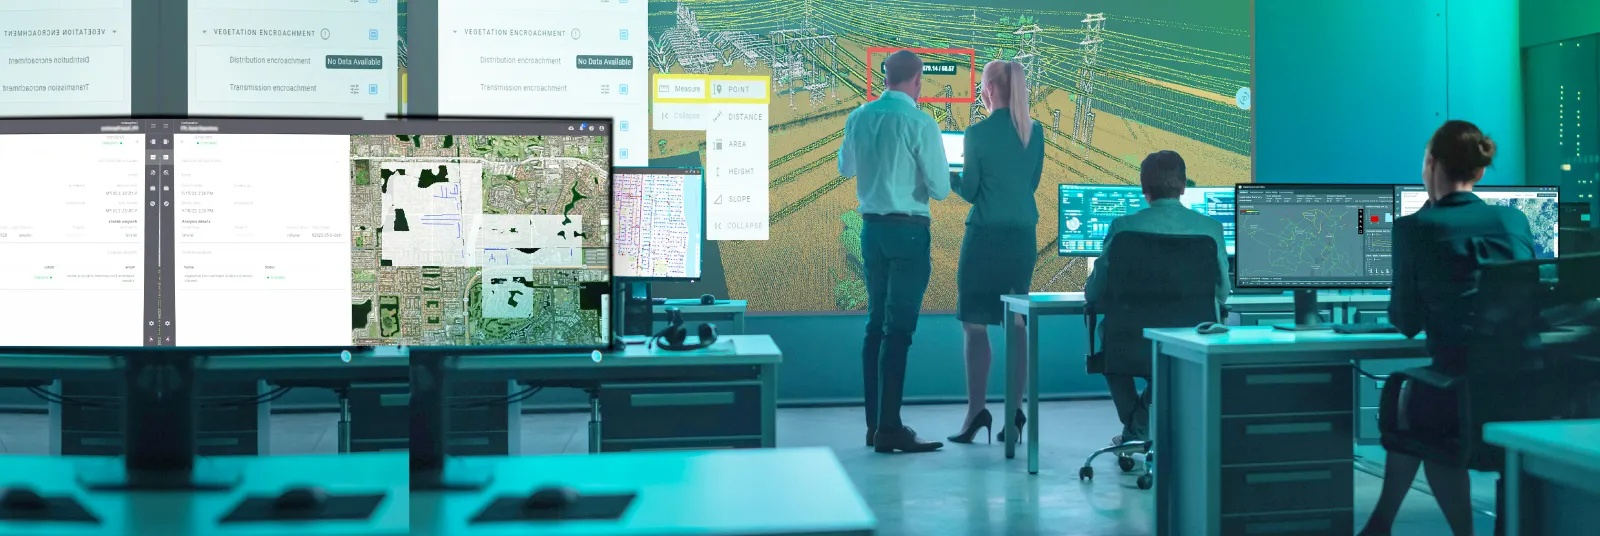
\includegraphics[width=\linewidth,height=3.85cm,keepaspectratio]{images/ge_gridos_control_room.jpg}
\par{\fontsize{7}{8.3}\selectfont\color{Slate} Official GridOS promotional composite. The platform example does not establish a measured agent-specific result.}
\par\endgroup\smallskip
\end{column}\end{columns}
\vfill
{\small\color{IEEEBlue}\textbf{For each case, identify the customer, task, agent's role and measured result.}\par}\smallskip
{\fontsize{6.3}{7.5}\selectfont\color{Slate} Source: \href{https://www.gevernova.com/news/press-releases/ge-vernova-launches-gridos-distribution-industrys}{GE Vernova. GE Vernova Launches GridOS for Distribution, the Industry's First Unified Solution for Grid Orchestration. 2026-02-03.}\par}
\note{This GE example concerns GE Vernova's electric-power business. The February 2026 GridOS announcement names a utility context. It does not establish a specific autonomous LLM controller. Our teaching example explains what an integrated agent would also need: clear tool interfaces, saved state, evidence checks and limits on its authority. Takeaway: For each case, identify the customer, task, agent's role and measured result.

GE Vernova. GE Vernova Launches GridOS for Distribution, the Industry's First Unified Solution for Grid Orchestration. 2026-02-03.
Full source: https://www.gevernova.com/news/press-releases/ge-vernova-launches-gridos-distribution-industrys

GE Vernova. GE Vernova: GE Vernova GridOS promotional control-room composite with people and grid software displays. Image accessed 17 October 2026.
Full source: https://www.gevernova.com/software/products/gridos}
\end{frame}

\begin{frame}[t]{Operators often work against a deadline}
\relax
\begin{columns}[T,onlytextwidth]\begin{column}{.515\textwidth}
{
\normalsize\begin{itemize}
\item A PNNL survey of 20 control-room operators reported that, on average, 61\% of tasks needed completion in under 30 minutes.
\item The survey had 75 questions. It gives no task count or statistical spread behind that average.
\item An assistant should reduce the time people spend finding and reviewing evidence within the task's deadline.
\end{itemize}\par}
\end{column}\begin{column}{.445\textwidth}
\begingroup\centering
\includegraphics[width=\linewidth,height=3.85cm,keepaspectratio]{images/duke_control_room.jpg}
\par{\fontsize{7}{8.3}\selectfont\color{Slate} Duke Energy control room, 2022. The PNNL survey is a separate study.}
\par\endgroup\smallskip
\end{column}\end{columns}
\vfill
{\small\color{IEEEBlue}\textbf{Measure the operator's total effort and deadline alongside AI response time.}\par}\smallskip
{\fontsize{6.3}{7.5}\selectfont\color{Slate} Source: \href{https://www.pnnl.gov/sites/default/files/media/file/PNNL_workshop_Presentation_Human_Factors_Virtual_Workshop_March_2023.pdf}{Corey Fallon, Brett Jefferson, Tyler Ryan. An Analysis of Grid Operators. Pacific Northwest National Laboratory. 2023-04-19.}\par}
\note{The 61\% is an average share of tasks performed or supported. It is not the percentage of operators. The source gives neither the task denominator nor variance. Twenty respondents do not support a binomial interval for that 61\%. Seventy-five survey items do not imply 1,500 independent timing observations. This small self-report study is not a national estimate. Ask which tasks need quick decisions and which allow more investigation. Takeaway: Measure the operator's total effort and deadline alongside AI response time.

Corey Fallon, Brett Jefferson, Tyler Ryan. An Analysis of Grid Operators. Pacific Northwest National Laboratory. 2023-04-19.
Full source: https://www.pnnl.gov/sites/default/files/media/file/PNNL\_workshop\_Presentation\_Human\_Factors\_Virtual\_Workshop\_March\_2023.pdf

PJM Interconnection. What Happens in the Control Room. 2026-04-16.
Full source: https://www.pjm.com/-/media/DotCom/about-pjm/newsroom/fact-sheets/what-happens-in-the-control-room-fact-sheet.pdf

Duke Energy / illumination. Duke Energy, illumination, August 2, 2022: Duke Energy employees in an Energy Control Center, with one pointing toward a display. Image accessed 17 October 2026.
Full source: https://illumination.duke-energy.com/articles/meet-the-team-that-monitors-the-grid-and-keeps-the-lights-on}
\end{frame}

\begin{frame}[t]{Three checks for a useful recommendation}
\relax
\begin{columns}[T,onlytextwidth]\begin{column}{.515\textwidth}
{
\normalsize\begin{itemize}
\item Data: do the asset, units, time and grid connections (topology) match the question?
\item Engineering: does the solution meet the requested equations and limits?
\item Decision: is there enough evidence for the next step the user is allowed to take?
\end{itemize}\par}
\end{column}\begin{column}{.445\textwidth}
\begingroup\centering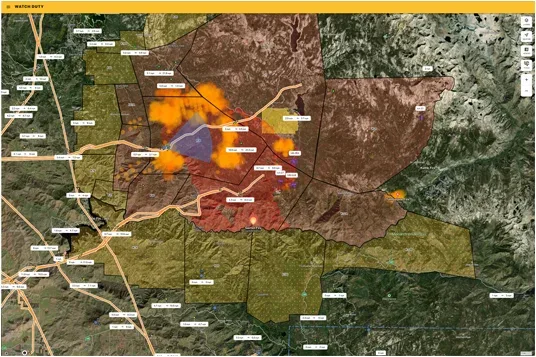
\includegraphics[width=\linewidth,height=3.85cm,keepaspectratio]{images/caiso_watch_duty.png}
\par{\fontsize{7}{8.3}\selectfont\color{Slate} Real CAISO Watch Duty display. It combines fire and transmission-line information for operator awareness.}
\par\endgroup\smallskip
\end{column}\end{columns}
\vfill
{\small\color{IEEEBlue}\textbf{Agree on acceptance checks for the whole task.}\par}\smallskip
{\fontsize{6.3}{7.5}\selectfont\color{Slate} Source: \href{https://www.caiso.com/about/news/energy-matters-blog/control-center-modernization-is-enhancing-reliability}{John Phipps. Control center modernization is enhancing reliability. California ISO. 2025-09-10.}\par}
\note{These are separate checks. A correctly formatted call may still use old grid connections. An optimization may converge after changing a variable the user was not allowed to change. A correct result may still leave part of the decision unanswered. These checks form the acceptance contract: the agreed conditions a result must meet. We reuse it in the examples and exercises. This original utility screenshot provides a concrete example of displayed evidence to inspect. It is conventional situational-awareness software, not an agent implementation or a claim that the slide's three checks were measured by CAISO. Takeaway: Agree on acceptance checks for the whole task.

John Phipps. Control center modernization is enhancing reliability. California ISO. 2025-09-10.
Full source: https://www.caiso.com/about/news/energy-matters-blog/control-center-modernization-is-enhancing-reliability}
\end{frame}

\begin{frame}[t]{A clear task makes success easier to test}
\relax
\begin{columns}[T,onlytextwidth]\begin{column}{.515\textwidth}
{
\normalsize\begin{itemize}
\item The task is to check whether an earlier study result still applies after a new event.
\item Return evidence or ask for missing data. Stop if inputs change, a tool fails, the work budget runs out or permission is missing.
\end{itemize}\par}
\end{column}\begin{column}{.445\textwidth}
\begingroup\centering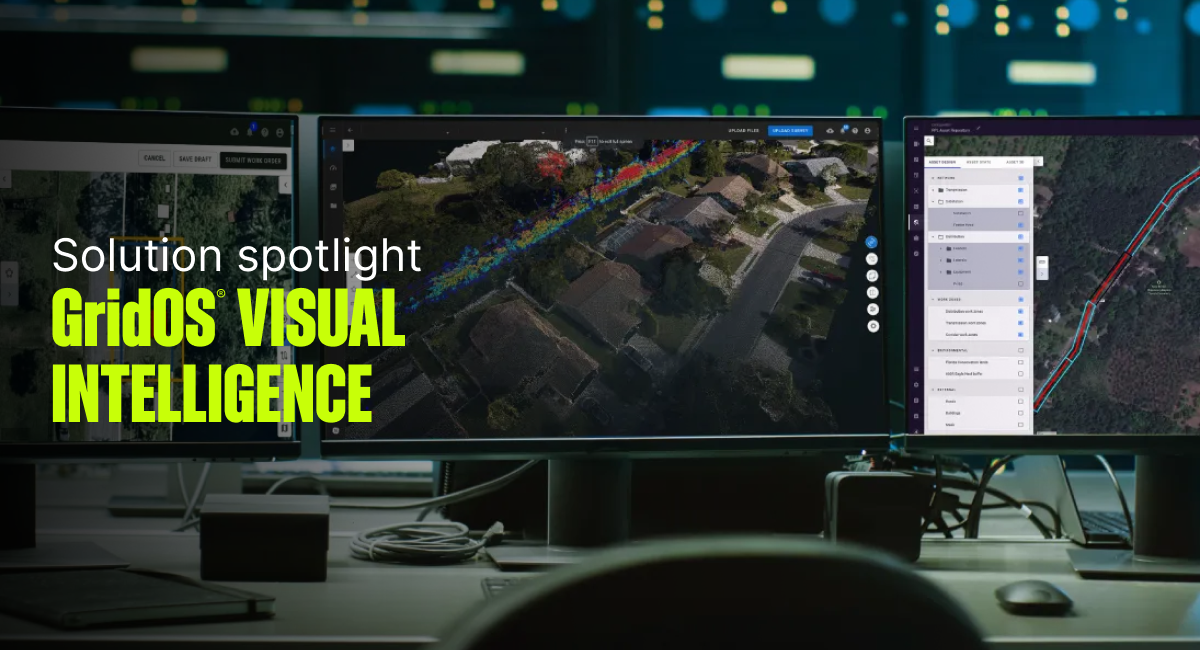
\includegraphics[width=\linewidth,height=3.85cm,keepaspectratio]{images/ge_gridos_visual_intelligence.png}
\par{\fontsize{7}{8.3}\selectfont\color{Slate} GE Vernova's published GridOS Visual Intelligence screen. This product image supplies task context, not an agent result.}
\par\endgroup\smallskip
\end{column}\end{columns}
\vfill
{\small\color{IEEEBlue}\textbf{A clear task gives us a clear way to check success.}\par}\smallskip
{\fontsize{6.3}{7.5}\selectfont\color{Slate} Source: \href{https://www.gevernova.com/software/products/gridos/visual-intelligence}{GE Vernova. GridOS Visual Intelligence product screens. Accessed 17 October 2026.}\par}
\note{All F12 records and policies are invented teaching data, not utility operating rules. A snapshot identifies the data time, grid-connection version and model revision. Start by identifying the user, the result they need and the actions they may take. Success means meeting these agreed requirements. Answer length and the number of tool calls do not establish success. The real product screen illustrates the grid information a bounded task may use. The acceptance contract on this slide remains an original teaching example. Takeaway: A clear task gives us a clear way to check success.

GE Vernova. GridOS Visual Intelligence product screens. Accessed 17 October 2026.
Full source: https://www.gevernova.com/software/products/gridos/visual-intelligence}
\end{frame}

\begin{frame}[t]{An LLM agent acts, reads the result and decides again}
\relax
\begingroup\centering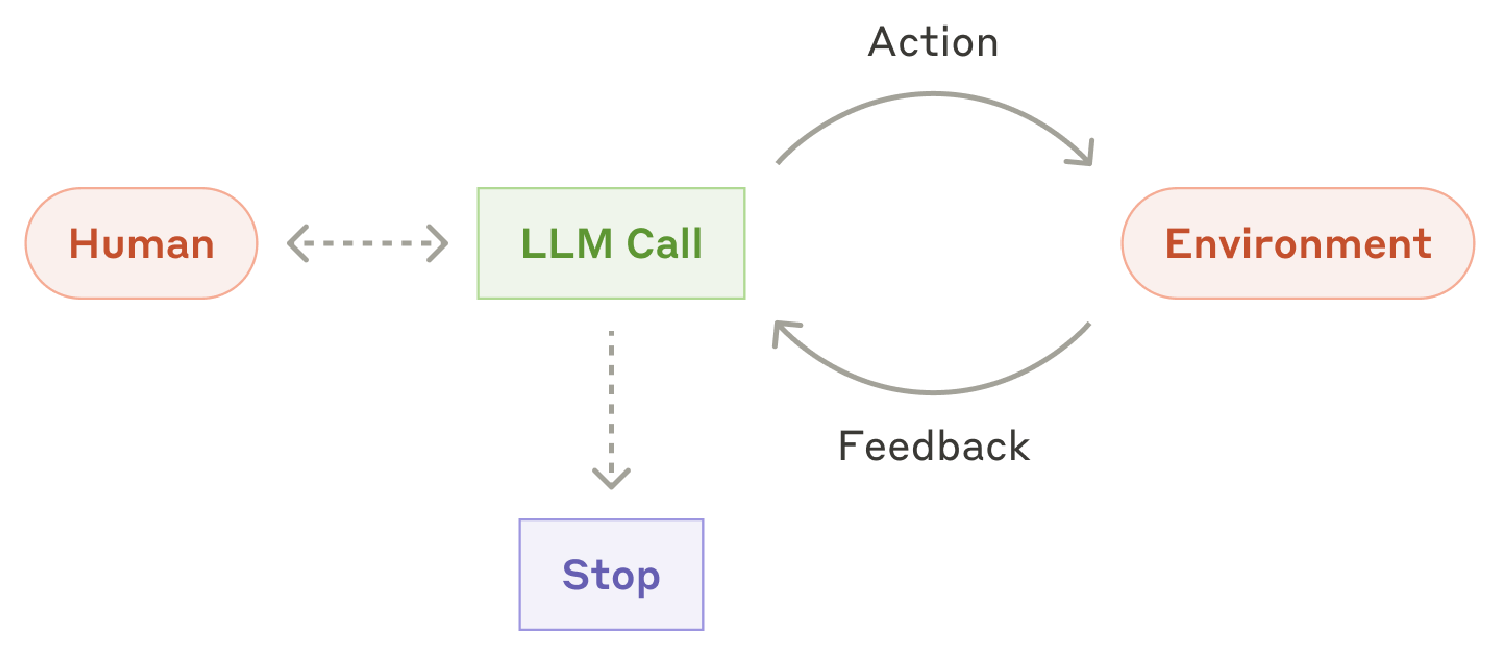
\includegraphics[width=\linewidth,height=4.05cm,keepaspectratio]{images/source_anthropic_autonomous_agent_wide.pdf}
\par{\fontsize{7}{8.3}\selectfont\color{Slate} Original Anthropic agent-loop figure. In a grid study, feedback can be solver results or a failed check.}
\par\endgroup\smallskip
{
\small\begin{itemize}
\setlength{\itemsep}{.25em}
\item After an action, the agent reads what happened before choosing the next step.
\item It can call another allowed tool, ask a person or stop. An error is also useful feedback.
\end{itemize}\par}
\vfill
{\fontsize{6.3}{7.5}\selectfont\color{Slate} Source: \href{https://www.anthropic.com/engineering/building-effective-agents}{Erik S., Barry Zhang. Building effective agents. Anthropic Engineering. 2024-12-19.}\par}
\note{The equation describes a software interface. It does not assume we observe the full physical system or that the history has the Markov property, meaning it contains everything needed to predict the next state. The model chooses a request using the goal and previous evidence. The software runs a service against a specific input snapshot. A historian, which stores time-stamped measurements, returns measured data. A simulator returns model results. Selecting either tool does not turn its output into a command to physical equipment. This is the original published conceptual agent pattern, not a measured utility or PowerAgent implementation. The display trims only empty margins. Feedback does not automatically mean model weights are being retrained. Takeaway: Check the tool requests, their inputs and their results.

Erik S., Barry Zhang. Building effective agents. Anthropic Engineering. 2024-12-19.
Full source: https://www.anthropic.com/engineering/building-effective-agents

LangChain documentation maintainers. LangGraph Graph API overview. Official LangChain documentation. Accessed 2026-10-17; live documentation.
Full source: https://docs.langchain.com/oss/python/langgraph/graph-api

Yihan (Logon) Wen, Xin Chen. X-GridAgent: An LLM-Powered Agentic AI System for Assisting Power Grid Analysis. arXiv preprint. 2025-12-23 (v1).
Full source: https://arxiv.org/pdf/2512.20789v1}
\end{frame}

\begin{frame}[t]{When data are stale, the next step is to stop}
\relax
\begingroup\centering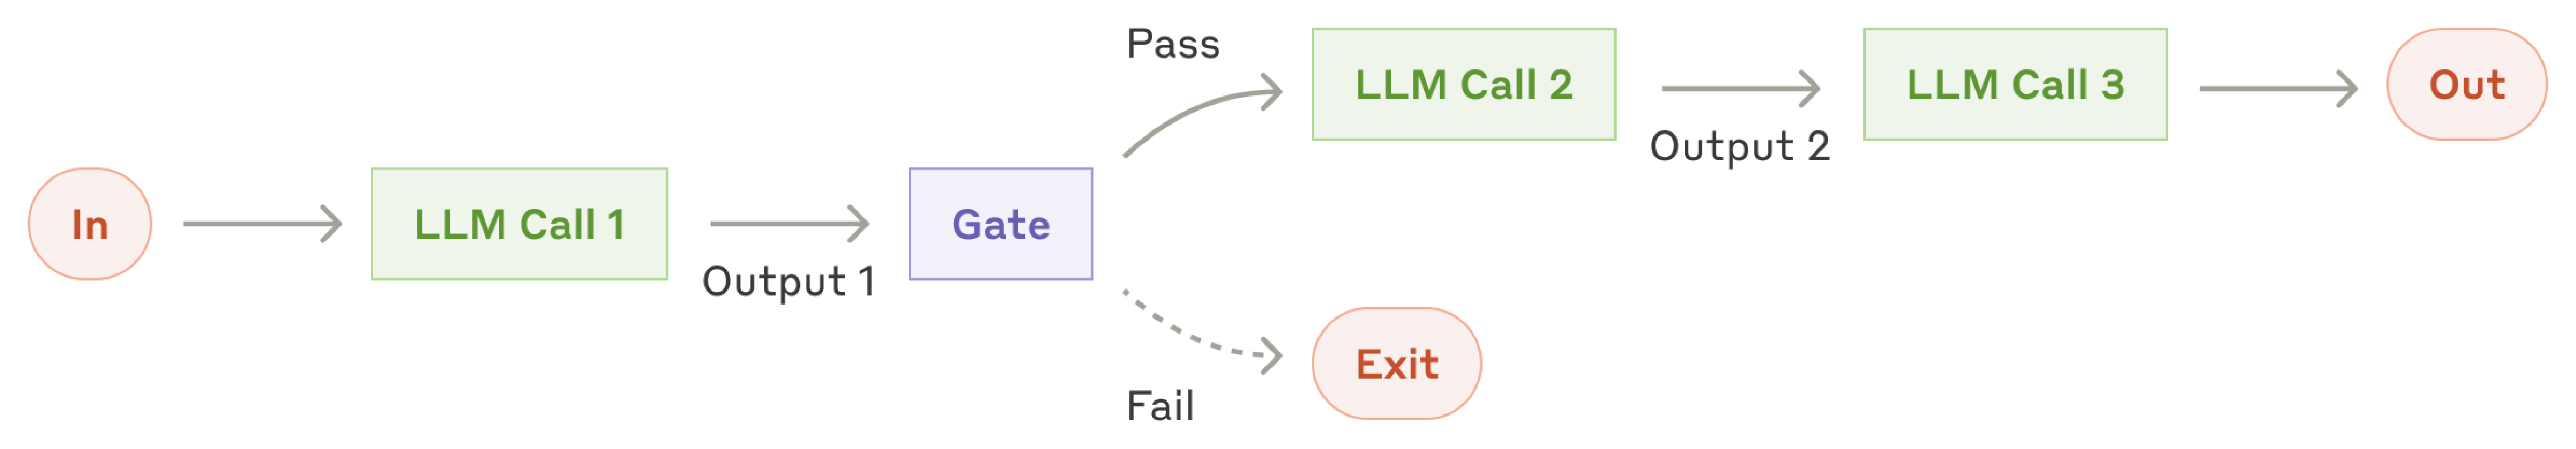
\includegraphics[width=\linewidth,height=3.7cm,keepaspectratio]{images/real_framework_anthropic_prompt_chain.pdf}
\par{\fontsize{7}{8.3}\selectfont\color{Slate} Original Anthropic gated workflow. In our study example, a stale input should fail the check and stop the sequence.}
\par\endgroup\smallskip
{
\small\begin{itemize}
\setlength{\itemsep}{.25em}
\item The asset lookup succeeds, but the measurement request marks the data as stale, meaning out of date.
\item Ask for current evidence. The original task remains unresolved.
\end{itemize}\par}
\vfill
{\fontsize{6.3}{7.5}\selectfont\color{Slate} Source: \href{https://www.anthropic.com/engineering/building-effective-agents}{Erik S., Barry Zhang. Building effective agents. Anthropic Engineering. 2024-12-19.}\par}
\note{A trace records the sequence of tool requests and results. Use the gate in this published figure to discuss an application check. As a spoken example, a study trace should record case IDs, data times and the returned results. When required data are unavailable or out of date, the system should say so. It must not invent a value or silently reuse an older one. Check whether the agent detects the problem and asks for the right update. A trace makes this inspection possible but does not itself prove the work is correct. Source: Anthropic, Building effective agents (December 19, 2024). A generic content-workflow pattern, not a physical-feasibility or utility-safety guarantee. Source figure locator: Workflow: Prompt chaining. Original source URL: https://www.anthropic.com/engineering/building-effective-agents Takeaway: 

Erik S., Barry Zhang. Building effective agents. Anthropic Engineering. 2024-12-19.
Full source: https://www.anthropic.com/engineering/building-effective-agents}
\end{frame}

\begin{frame}[t]{Unit checks catch a kV versus p.u. mistake}
\relax
\begingroup\begin{minipage}[c][4cm][c]{\linewidth}\centering\setbox0=\hbox{\resizebox{.96\linewidth}{!}{\begin{tikzpicture}[x=1cm,y=1cm,font=\sffamily\fontsize{12}{14}\selectfont,
  line cap=round,line join=round,
  rp/.style={circle,draw=rBlue,fill=white,minimum size=5.4mm,inner sep=0pt,line width=1.15pt},
  rl/.style={align=center,text=rNavy,font=\sffamily\bfseries\fontsize{12.5}{14.5}\selectfont},
  rn/.style={align=center,text=rNavy,font=\sffamily\fontsize{11.2}{13}\selectfont},
  rc/.style={align=left,text=rNavy,font=\ttfamily\fontsize{11}{13}\selectfont},
  rf/.style={-{Latex[length=2mm,width=1.5mm]},draw=rBlue,line width=1.15pt,shorten >=1.4pt,shorten <=1.4pt},
  rw/.style={-{Latex[length=2mm,width=1.5mm]},draw=rOrange,line width=1.15pt,shorten >=1.4pt,shorten <=1.4pt}]
\definecolor{rBlue}{HTML}{00629B}
\definecolor{rCyan}{HTML}{00A8C8}
\definecolor{rNavy}{HTML}{003B5C}
\definecolor{rOrange}{HTML}{B65B14}
\definecolor{rGray}{HTML}{74828C}
\path[use as bounding box] (0,0) rectangle (14.2,4.2);

\node[rc,anchor=west] at (0.3,3.55) {asset=F12, voltage=12.47 kV};
\node[rc,anchor=west] at (0.3,2.95) {topology=v42};
\node[rp] (badgate) at (8.45,3.25) {};
\draw[rf] (6.7,3.25) -- (badgate.west);
\draw[rw] (badgate.east) -- (10.4,3.25);
\node[rl,text=rOrange,anchor=west] at (10.65,3.25) {REJECT};
\node[rn,text=rOrange] at (11.4,2.55) {expects pu + v43};
\node[rn] at (8.45,3.88) {Validator};
\draw[draw=rGray,line width=0.5pt] (0.3,2.12) -- (13.8,2.12);
\node[rc,anchor=west] at (0.3,1.65) {asset=F12, voltage=1.00 pu};
\node[rc,anchor=west] at (0.3,1.05) {base=12.47 kV, topology=v43};
\node[rp] (goodgate) at (8.45,1.35) {};
\draw[rf] (6.7,1.35) -- (goodgate.west);
\draw[rf] (goodgate.east) -- (11.45,1.35);
\node[rl,anchor=west] at (11.7,1.35) {Solver};
\node[rn] at (8.45,0.8) {valid request};
\node[rn] at (7.1,0.2) {12.47 kV / 12.47 kV = 1.00 pu, using the same voltage base};

\end{tikzpicture}
}}\ifdim\dimexpr\ht0+\dp0\relax>4cm\resizebox{!}{4cm}{\box0}\else\box0\fi\par\end{minipage}
{\fontsize{7}{8.3}\selectfont\color{Slate} Teaching example with invented values. These values are not recommended operating limits.\par}
\endgroup\smallskip
{
\small\begin{itemize}
\setlength{\itemsep}{.25em}
\item 12.47 kV is 1.00 per unit (p.u.) only with a 12.47 kV base. Per unit means value divided by base.
\item A tool expecting p.u. must reject a raw kV value or require explicit information for converting it.
\end{itemize}\par}
\vfill
\note{The software interface must enforce units. Prompt wording alone is insufficient. The same number can mean very different physical quantities. Check unit labels, the chosen base and the asset ID in software. A valid type or unit still does not prove that the measurement or model is accurate. The diagram shows both the error and the information needed to fix it. Takeaway: 

}
\end{frame}

\begin{frame}[t]{A study must match the current grid connections}
\relax
\begingroup\begin{minipage}[c][4cm][c]{\linewidth}\centering\setbox0=\hbox{\resizebox{.96\linewidth}{!}{\begin{tikzpicture}[x=1cm,y=1cm,font=\sffamily\fontsize{12}{14}\selectfont,
  line cap=round,line join=round,
  rp/.style={circle,draw=rBlue,fill=white,minimum size=5.4mm,inner sep=0pt,line width=1.15pt},
  rl/.style={align=center,text=rNavy,font=\sffamily\bfseries\fontsize{12.5}{14.5}\selectfont},
  rn/.style={align=center,text=rNavy,font=\sffamily\fontsize{11.2}{13}\selectfont},
  rc/.style={align=left,text=rNavy,font=\ttfamily\fontsize{11}{13}\selectfont},
  rf/.style={-{Latex[length=2mm,width=1.5mm]},draw=rBlue,line width=1.15pt,shorten >=1.4pt,shorten <=1.4pt},
  rw/.style={-{Latex[length=2mm,width=1.5mm]},draw=rOrange,line width=1.15pt,shorten >=1.4pt,shorten <=1.4pt}]
\definecolor{rBlue}{HTML}{00629B}
\definecolor{rCyan}{HTML}{00A8C8}
\definecolor{rNavy}{HTML}{003B5C}
\definecolor{rOrange}{HTML}{B65B14}
\definecolor{rGray}{HTML}{74828C}
\path[use as bounding box] (0,0) rectangle (14.2,4.2);

\node[rl] at (3.1,3.75) {14:35 snapshot: v42};
\node[rl] at (10.7,3.75) {15:02 event: v43};
\node[rp] (a1) at (0.85,2.65) {A};
\node[rp] (b1) at (5.35,2.65) {B};
\node[rp] (a2) at (8.25,2.65) {A};
\node[rp] (b2) at (12.75,2.65) {B};
\draw[draw=rBlue,line width=1.2pt] (a1.east) -- (2.6,2.65);
\draw[draw=rBlue,line width=1.2pt] (3.6,2.65) -- (b1.west);
\fill[rBlue] (2.6,2.65) circle (1.7pt);
\fill[rBlue] (3.6,2.65) circle (1.7pt);
\draw[draw=rBlue,line width=1.6pt] (2.6,2.65) -- (3.6,2.65);
\draw[draw=rBlue,line width=1.2pt] (a2.east) -- (10.0,2.65);
\draw[draw=rBlue,line width=1.2pt] (11.0,2.65) -- (b2.west);
\fill[rOrange] (10.0,2.65) circle (1.7pt);
\fill[rOrange] (11.0,2.65) circle (1.7pt);
\draw[draw=rOrange,line width=1.6pt] (10.0,2.65) -- (10.85,3.18);
\draw[rf] (6.1,2.65) -- (7.5,2.65);
\node[rn] at (6.8,3.15) {S opens};
\node[rl] at (3.1,1.95) {S closed};
\node[rl,text=rOrange] at (10.5,1.95) {S open};
\node[rn] at (3.1,1.1) {14:40 study uses v42};
\node[rn] at (10.5,1.1) {15:05 review sees v43};
\draw[draw=rOrange,line width=1.0pt] (2.2,0.7) -- (12.1,0.7);
\node[rl,text=rOrange] at (7.1,0.22) {Old result needs revalidation against the changed topology};

\end{tikzpicture}
}}\ifdim\dimexpr\ht0+\dp0\relax>4cm\resizebox{!}{4cm}{\box0}\else\box0\fi\par\end{minipage}
{\fontsize{7}{8.3}\selectfont\color{Slate} Invented before-and-after network. This illustration does not calculate power flow.\par}
\endgroup\smallskip
{
\small\begin{itemize}
\setlength{\itemsep}{.25em}
\item The old study used a closed switch and grid version v42. The event opens the switch and creates version v43.
\item Update the inputs and repeat the affected calculations. Rewriting the explanation does not update the numerical result.
\end{itemize}\par}
\vfill
\note{Point to the switch that changed. The old result represents different grid connections, rather than simply an older timestamp. Version matching is a necessary consistency check. It still leaves two questions: does the model represent the real grid accurately, and do the refreshed measurements represent the event? Takeaway: 

}
\end{frame}

\begin{frame}[t]{A solver result depends on the problem it solves}
\relax
\begin{columns}[T,onlytextwidth]\begin{column}{.64\textwidth}
\begingroup\centering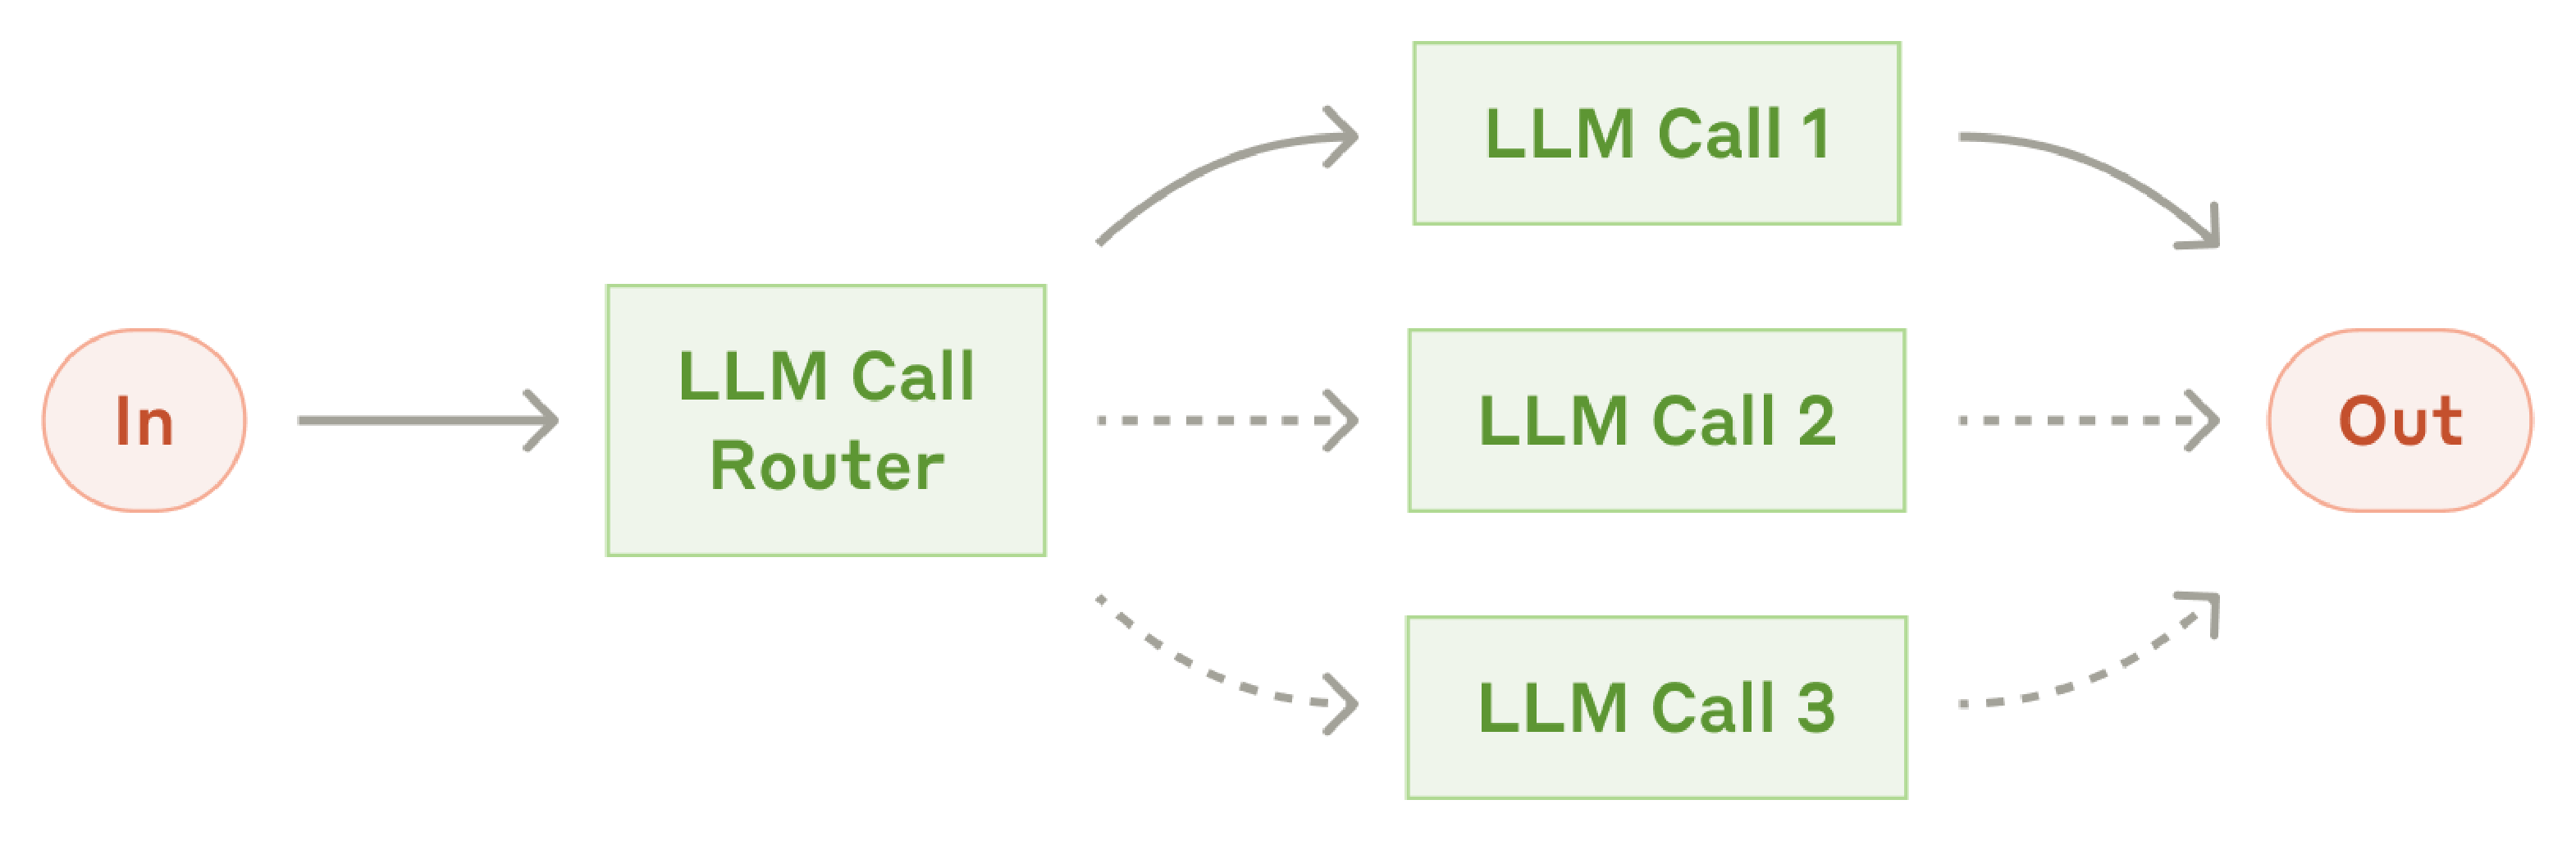
\includegraphics[width=\linewidth,height=4.65cm,keepaspectratio]{images/real_framework_anthropic_routing.pdf}
\par{\fontsize{7}{8.3}\selectfont\color{Slate} Original Anthropic routing pattern. Choosing an engineering study also requires selecting the right problem and tool.}
\par\endgroup\smallskip
\end{column}\begin{column}{.32\textwidth}
{
\small\begin{itemize}
\setlength{\itemsep}{.25em}
\item Choose the study first: power flow, optimal dispatch and dynamic simulation answer different questions.
\item A solver's success flag covers that problem. Also check the requested cases, grid limits and permission to act.
\end{itemize}\par}
\end{column}\end{columns}
\vfill
{\fontsize{6.3}{7.5}\selectfont\color{Slate} Source: \href{https://arxiv.org/abs/2609.04544v1}{Samim Konjicija, Slaven Peles. Integrating Agentic Artificial Intelligence with High-Performance Computing for Grid Planning. arXiv; EnergyCon 2026 proceedings forthcoming as described by authors. 3 September 2026; v1.}\par}
\note{Keep solver status, equation errors (residuals) and modeled limit checks separate from whether the analysis covers the full request. A solver can converge on the wrong problem. The study requirements must state constraints and tolerances, meaning the allowed numerical error. This slide sets no universal voltage or loading limit. Permission to act remains a separate software and organizational decision. Source: Anthropic, Building effective agents (December 19, 2024). The picture illustrates routing; it does not establish an implemented power-system workflow. Source figure locator: Workflow: Routing. Original source URL: https://www.anthropic.com/engineering/building-effective-agents Takeaway: Report the problem and assumptions together with the solver result.

Samim Konjicija, Slaven Peles. Integrating Agentic Artificial Intelligence with High-Performance Computing for Grid Planning. arXiv; EnergyCon 2026 proceedings forthcoming as described by authors. 3 September 2026; v1.
Full source: https://arxiv.org/abs/2609.04544v1
Full paper: https://arxiv.org/pdf/2609.04544v1

GridGuard project / local source snapshot. GridGuard current project: README and graph source snapshot. 2026.
Full source: ../research/GridGuard\_source\_snapshot.txt

Erik S., Barry Zhang. Building effective agents. Anthropic Engineering. 2024-12-19.
Full source: https://www.anthropic.com/engineering/building-effective-agents}
\end{frame}

\begin{frame}[t]{Exercise 1: check three returned data packets}
\relax
{\scriptsize\color{Slate}\textbf{Work in pairs / 6 minutes}\par}\smallskip
\begingroup\fontsize{10}{13}\selectfont\ttfamily\raggedright
\noindent\strut\mbox{A~=~\{age\_s:20,~topology:v42,~unit:pu\}}\par
\noindent\strut\mbox{B~=~\{age\_s:15,~topology:v43,~unit:kV\}}\par
\noindent\strut\mbox{C~=~\{age\_s:45,~topology:v43,~unit:pu\}}\par
\endgroup\medskip
{
\normalsize\begin{itemize}
\item For this exercise, data must be at most 60 s old, use topology v43 and use p.u. The user can recommend actions only.
\item Which packet passes? Explain why each other packet fails.
\item Does passing these checks establish complete engineering validity or permission to execute an action?
\end{itemize}\par}
\vfill
\note{Allow 1 minute to inspect, 2 minutes in pairs, 2 minutes to share and 1 minute to debrief. age\_s means age in seconds. Only C passes the stated initial checks. A has the wrong grid version. B has the wrong unit. C still needs the right asset mapping, a valid model, the required engineering checks, enough scenario coverage and an explanation people can review. The user may advise but cannot execute actions. The 60-second rule is made up for this exercise. It is not a general operating standard. Takeaway: 

}
\end{frame}

\begin{frame}[t]{Power-system papers test different tasks}
\relax
\begin{columns}[T,onlytextwidth]\begin{column}{.515\textwidth}
{
\normalsize\begin{itemize}
\item Fault-analysis tools find events in recorded waveforms. Simulation assistants set up and run studies.
\item Control prototypes suggest actions in model grids. Benchmarks test how well systems find evidence or answer numerical questions.
\item Each result applies to the tested task, tools, allowed actions and test cases.
\end{itemize}\par}
\end{column}\begin{column}{.445\textwidth}
\begingroup\centering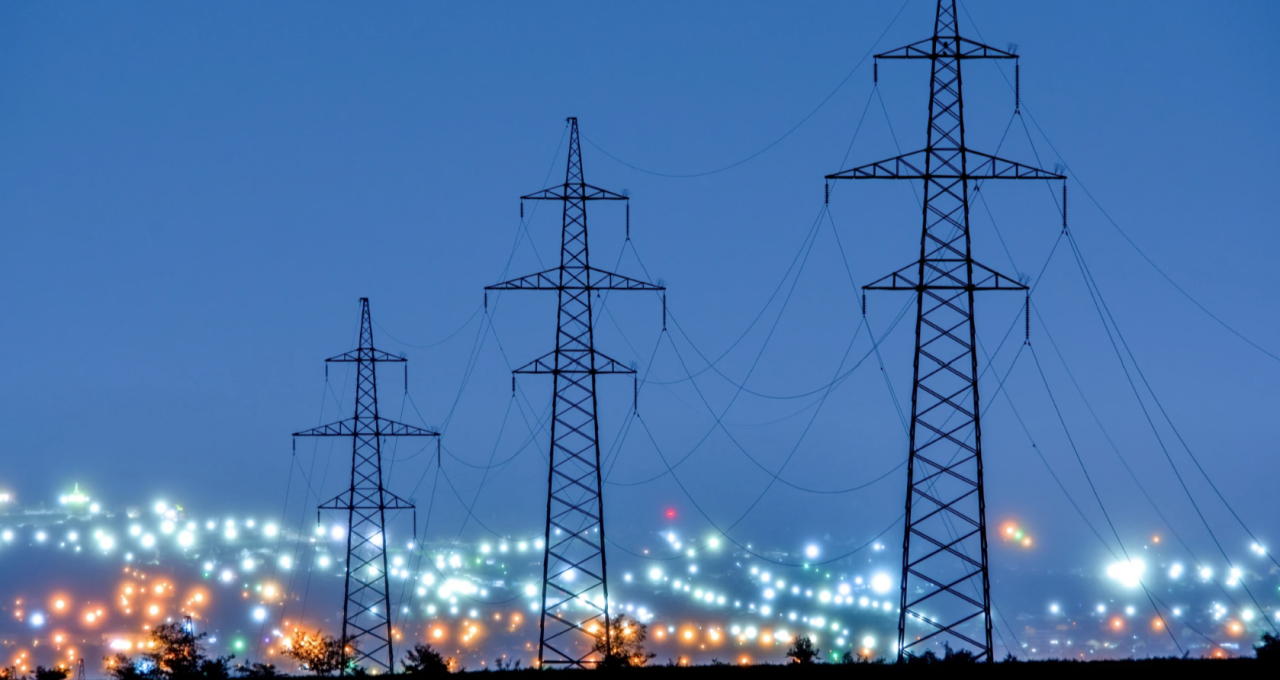
\includegraphics[width=\linewidth,height=3.85cm,keepaspectratio]{images/epri_open_power_ai_grid.png}
\par{\fontsize{7}{8.3}\selectfont\color{Slate} Image accompanying the EPRI Open Power AI Consortium announcement, published by NVIDIA, 20 March 2025.}
\par\endgroup\smallskip
\end{column}\end{columns}
\vfill
{\fontsize{6.3}{7.5}\selectfont\color{Slate} Source: \href{https://www.manuscriptlink.com/society/kics/media?key=kics\%2Fconference\%2Ficaiic2025\%2Fpresentation\%2F1571098105.pdf}{Barun Kumar Saha, Aarthi V, O. D. Naidu. DrAgent: An Agentic Approach to Fault Analysis in Power Grids Using Large Language Models. 2025 International Conference on Artificial Intelligence in Information and Communication (ICAIIC), pp. 938--945. 2025-02-18--21.}\par}
\note{Every paper that follows concerns power systems. They measure different outcomes, so their percentages cannot form a ranking across papers. The numerical solver computes the engineering result. The language model selects tools and helps interpret the returned evidence. This source photograph introduces the power-sector research context. It does not picture the paper experiments. Takeaway: 

Barun Kumar Saha, Aarthi V, O. D. Naidu. DrAgent: An Agentic Approach to Fault Analysis in Power Grids Using Large Language Models. 2025 International Conference on Artificial Intelligence in Information and Communication (ICAIIC), pp. 938--945. 2025-02-18--21.
Full source: https://www.manuscriptlink.com/society/kics/media?key=kics\%2Fconference\%2Ficaiic2025\%2Fpresentation\%2F1571098105.pdf
Publication: https://doi.org/10.1109/ICAIIC64266.2025.10920654

Mengshuo Jia, Zeyu Cui, Gabriela Hug. Enhancing LLMs for Power System Simulations: A Feedback-Driven Multi-Agent Framework. IEEE Transactions on Smart Grid, volume 16, issue 6, pages 5556--5572. 2025.
Full source: https://doi.org/10.1109/TSG.2025.3589114
Full paper: https://arxiv.org/pdf/2411.16707v3

Yan Zhang, Ahmad Mohammad Saber, Amr Youssef, Deepa Kundur. Grid-Agent: An LLM-Powered Multi-Agent System for Power Grid Control. arXiv preprint. 2025-09-08 (v3); first submitted 2025-08-07.
Full source: https://arxiv.org/pdf/2508.05702v3

Xijing Wang, Yinsheng Yao, Jinru Ding, Yidong Jiang, Ziwen Xu, Yiwen Jiang, Jie Xu, Dawei Cheng. PowerBench: A Benchmark for Agentic Retrieval and Reasoning in Power Systems. arXiv. 2026-09-28 (v1).
Full source: https://arxiv.org/abs/2609.34492v1
Full paper: https://arxiv.org/pdf/2609.34492v1

NVIDIA. Image published by NVIDIA with its EPRI Open Power AI Consortium announcement, March 20, 2025: Transmission towers and power lines with city lights in the background at dusk. Image accessed 17 October 2026.
Full source: https://blogs.nvidia.com/blog/open-power-ai-consortium/}
\end{frame}

\begin{frame}[t]{Harvard PowerAgent: models, tools and study workflows}
\relax
\begin{columns}[T,onlytextwidth]\begin{column}{.64\textwidth}
\begingroup\centering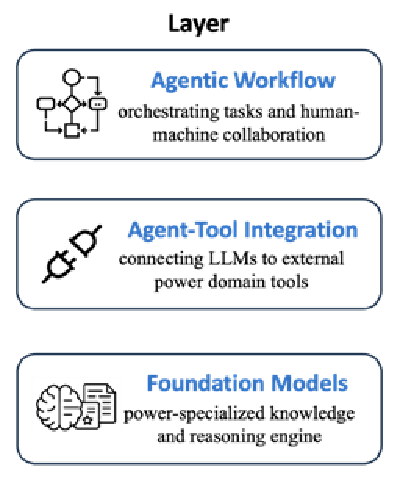
\includegraphics[width=\linewidth,height=4.6cm,keepaspectratio]{images/real_paper_poweragent_three_layers.pdf}
\par{\fontsize{7}{8.3}\selectfont\color{Slate} Original Harvard author roadmap: workflows, tool connections and foundation models. Three-layer excerpt.}
\par\endgroup\smallskip
\end{column}\begin{column}{.32\textwidth}
{
\small\begin{itemize}
\setlength{\itemsep}{.25em}
\item PowerAgent's 2025 IEEE roadmap links AI models, power tools and study workflows.
\item PowerFM supports modeling. PowerMCP connects tools. PowerWF manages workflows. PowerAgentBench-Dyn is a later benchmark, not the whole initiative.
\end{itemize}\par}
\end{column}\end{columns}
\vfill
{\fontsize{6.3}{7.5}\selectfont\color{Slate} Source: \href{https://doi.org/10.1109/MPE.2025.3579718}{Qian Zhang, Le Xie. PowerAgent: A Road Map Toward Agentic Intelligence in Power Systems: Foundation Model, Model Context Protocol, and Workflow. IEEE Power and Energy Magazine, volume 23, issue 5, pages 93--101. 2025.}\par}
\note{Full citation: Qian Zhang and Le Xie, PowerAgent: A Road Map Toward Agentic Intelligence in Power Systems: Foundation Model, Model Context Protocol, and Workflow, IEEE Power and Energy Magazine 23(5), 93--101, September--October 2025, DOI 10.1109/MPE.2025.3579718. A foundation model is a pretrained model intended for reuse across tasks. We verified the architecture through the authors' full ERCOT presentation and official project page. The publisher/preprint download was unavailable, so we attribute no uninspected experimental results to the article. The community and repositories keep changing. Their current features are not a fixed 2025 benchmark. Le Xie; slides credit Le Xie and Qian Zhang; A Roadmap Towards Agentic Intelligence in Power Systems; Author presentation slide 11 Roadmap from the December2025 author presentation; not a measured deployment or a frozen specification of every current PowerAgent repository. Source locator: Author presentation slide 11; three layer panels in the left column. Original URL: https://www.ercot.com/files/docs/2025/12/01/4-Guest-Presentation-A-Roadmap-toward-Agentic-Intelligence-in-Power-Systems.pdf Takeaway: 

Qian Zhang, Le Xie. PowerAgent: A Road Map Toward Agentic Intelligence in Power Systems: Foundation Model, Model Context Protocol, and Workflow. IEEE Power and Energy Magazine, volume 23, issue 5, pages 93--101. 2025.
Full source: https://doi.org/10.1109/MPE.2025.3579718

Le Xie; slides credit Le Xie and Qian Zhang. A Roadmap Towards Agentic Intelligence in Power Systems. ERCOT Technology and Security Committee guest presentation. 8 December 2025.
Full source: https://www.ercot.com/files/docs/2025/12/01/4-Guest-Presentation-A-Roadmap-toward-Agentic-Intelligence-in-Power-Systems.pdf

Power and AI Initiative / PowerAgent community, Harvard SEAS. PowerAgent --- Open-Source Agentic AI for Power Grids. Official Harvard project website. Live project page reviewed 17 October 2026.
Full source: https://poweragent.seas.harvard.edu/

Qian Zhang, Andrea Pomarico, Costas Mylonas, Magda Foti, Alberto Berizzi, Le Xie. PowerAgentBench-Dyn: A Benchmark for Agentic AI in Power System Dynamic Studies. arXiv. 2026-06-18 (v1).
Full source: https://arxiv.org/abs/2606.20401v1
Full paper: https://arxiv.org/pdf/2606.20401v1}
\end{frame}

\begin{frame}[t]{PowerAgent example: what changes when load is added?}
\relax
\begin{columns}[T,onlytextwidth]\begin{column}{.64\textwidth}
\begingroup\centering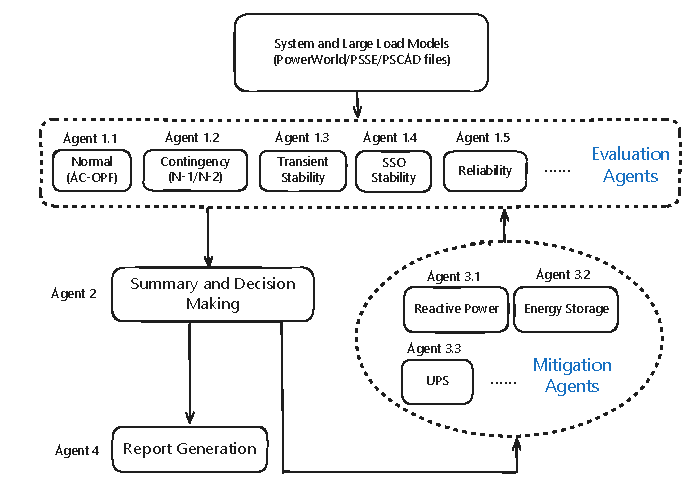
\includegraphics[width=\linewidth,height=4.6cm,keepaspectratio]{images/real_paper_poweragent_impact_workflow.pdf}
\par{\fontsize{7}{8.3}\selectfont\color{Slate} Original Harvard concept for grid-impact studies. The separate PowerWF example uses LangGraph and PowerWorld; this is not its exact graph.}
\par\endgroup\smallskip
\end{column}\begin{column}{.32\textwidth}
{
\small\begin{itemize}
\setlength{\itemsep}{.25em}
\item It runs power flow and single-outage checks (N-1) for the original case and the added-load case.
\item LangGraph manages the steps and saved results. PowerWorld calculates the electrical results.
\end{itemize}\par}
\end{column}\end{columns}
\vfill
{\fontsize{6.3}{7.5}\selectfont\color{Slate} Source: \href{https://github.com/Power-Agent/PowerWF/blob/main/Grid\%20Impact\%20Evaluation/src/agent/graph.py}{PowerAgent / PowerWF community contributors. PowerWF Grid Impact Evaluation --- LangGraph workflow source. Author-maintained source code, Grid Impact Evaluation/src/agent/graph.py. Live source inspected 17 October 2026.}\par}
\note{This is a specific current workflow maintained by the authors. It does not establish one SDK for the whole PowerAgent initiative. In the code, graph.py imports StateGraph and ToolNode, saves workflow flags and returns from the shared tools node to the relevant step. A bus is a connection point in the model. The author presentation discusses load-growth and data-center studies using power flow, congestion, voltage and N-1 checks, which examine single-component outages. The code and demonstrations show the workflow. They provide no controlled utility timing or reliability estimate. The reading guide links the exact source file. Le Xie; slides credit Le Xie and Qian Zhang; A Roadmap Towards Agentic Intelligence in Power Systems; Author presentation slide 14, right-hand grid-impact process A conceptual author demonstration. It is not an exact diagram of the later PowerWF graph.py or a utility performance trial. Source locator: Author presentation slide 14, right-hand grid-impact process. Original URL: https://www.ercot.com/files/docs/2025/12/01/4-Guest-Presentation-A-Roadmap-toward-Agentic-Intelligence-in-Power-Systems.pdf Takeaway: 

PowerAgent / PowerWF community contributors. PowerWF Grid Impact Evaluation --- LangGraph workflow source. Author-maintained source code, Grid Impact Evaluation/src/agent/graph.py. Live source inspected 17 October 2026.
Full source: https://github.com/Power-Agent/PowerWF/blob/main/Grid\%20Impact\%20Evaluation/src/agent/graph.py

Le Xie; slides credit Le Xie and Qian Zhang. A Roadmap Towards Agentic Intelligence in Power Systems. ERCOT Technology and Security Committee guest presentation. 8 December 2025.
Full source: https://www.ercot.com/files/docs/2025/12/01/4-Guest-Presentation-A-Roadmap-toward-Agentic-Intelligence-in-Power-Systems.pdf

PowerAgent community contributors. Power-Agent/PowerWF. Author-maintained GitHub repository. Live source repository reviewed 17 October 2026.
Full source: https://github.com/Power-Agent/PowerWF}
\end{frame}

\begin{frame}[t]{DrAgent: reading a recorded grid fault}
\relax
\begingroup\centering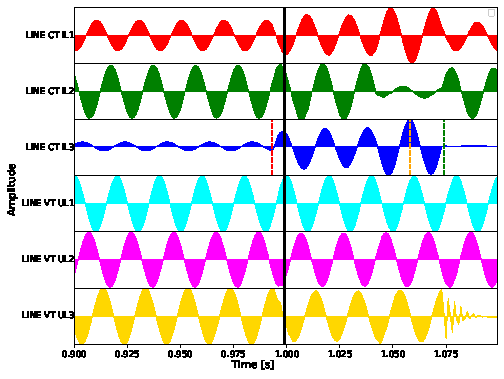
\includegraphics[width=\linewidth,height=4.15cm,keepaspectratio]{images/power_dragent_waveform.pdf}
\par{\fontsize{7}{8.3}\selectfont\color{Slate} Original DrAgent Figure 2, PDF p.4. The third current channel shows a fault in a sample disturbance record.}
\par\endgroup\smallskip
{
\small\begin{itemize}
\setlength{\itemsep}{.25em}
\item The third current trace shows the fault. Dashed lines mark its start, highest current and clearance (when the fault ends).
\end{itemize}\par}
\vfill
{\fontsize{6.3}{7.5}\selectfont\color{Slate} Source: \href{https://www.manuscriptlink.com/society/kics/media?key=kics\%2Fconference\%2Ficaiic2025\%2Fpresentation\%2F1571098105.pdf}{Barun Kumar Saha, Aarthi V, O. D. Naidu. DrAgent: An Agentic Approach to Fault Analysis in Power Grids Using Large Language Models. 2025 International Conference on Artificial Intelligence in Information and Communication (ICAIIC), pp. 938--945. 2025-02-18--21.}\par}
\note{The Hitachi Energy paper studies disturbance analysis on transmission lines. This is an original figure extracted from the research paper, not an invented event or a live operating screen. First identify how the curve changes. Numerical tools return a sample index or current measurement. The task still requires an engineering interpretation of those values. Takeaway: 

Barun Kumar Saha, Aarthi V, O. D. Naidu. DrAgent: An Agentic Approach to Fault Analysis in Power Grids Using Large Language Models. 2025 International Conference on Artificial Intelligence in Information and Communication (ICAIIC), pp. 938--945. 2025-02-18--21.
Full source: https://www.manuscriptlink.com/society/kics/media?key=kics\%2Fconference\%2Ficaiic2025\%2Fpresentation\%2F1571098105.pdf
Publication: https://doi.org/10.1109/ICAIIC64266.2025.10920654}
\end{frame}

\begin{frame}[t]{DrAgent selects tools to answer a fault question}
\relax
\begin{columns}[T,onlytextwidth]\begin{column}{.64\textwidth}
\begingroup\centering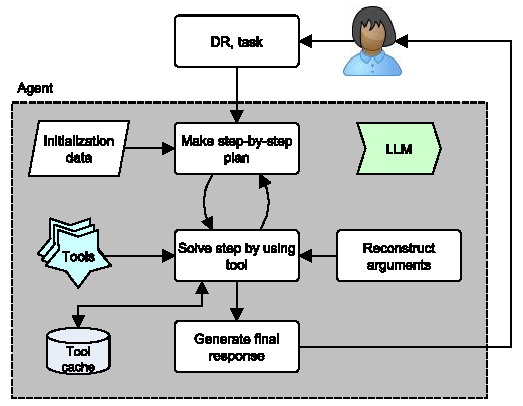
\includegraphics[width=\linewidth,height=4.6cm,keepaspectratio]{images/real_paper_dragent_architecture.pdf}
\par{\fontsize{7}{8.3}\selectfont\color{Slate} Original DrAgent architecture: planning, tool execution and answer generation.}
\par\endgroup\smallskip
\end{column}\begin{column}{.32\textwidth}
{
\small\begin{itemize}
\setlength{\itemsep}{.25em}
\item The plan chooses signal-analysis tools or manual search to match the question.
\item Signal tools measure the fault. Manual search finds product information in documents.
\end{itemize}\par}
\end{column}\end{columns}
\vfill
{\fontsize{6.3}{7.5}\selectfont\color{Slate} Source: \href{https://www.manuscriptlink.com/society/kics/media?key=kics\%2Fconference\%2Ficaiic2025\%2Fpresentation\%2F1571098105.pdf}{Barun Kumar Saha, Aarthi V, O. D. Naidu. DrAgent: An Agentic Approach to Fault Analysis in Power Grids Using Large Language Models. 2025 International Conference on Artificial Intelligence in Information and Communication (ICAIIC), pp. 938--945. 2025-02-18--21.}\par}
\note{ReWOO plans the work before running tools that use earlier results. COMTRADE is a format for recorded power-system disturbances. The implementation uses Gemini 1.5Pro for planning, a dozen domain functions and retrieval-augmented generation (RAG) over 138 product manuals. RAG retrieves relevant source text for the model. The displayed picture is the paper's original architecture. The following dependency example is a spoken teaching example. To convert a fault's starting sample to seconds, the system first needs both the sample index and sampling rate. This dependency motivates the next graph explanation. Barun Kumar Saha, Aarthi V, O. D. Naidu; DrAgent: An Agentic Approach to Fault Analysis in Power Grids Using Large Language Models; Figure 1, PDF page 2 Paper architecture based on ReWOO; the picture does not establish utility deployment or autonomous command authority. Source locator: Figure 1, PDF page 2. Original URL: https://www.manuscriptlink.com/society/kics/media?key=kics\%2Fconference\%2Ficaiic2025\%2Fpresentation\%2F1571098105.pdf Takeaway: 

Barun Kumar Saha, Aarthi V, O. D. Naidu. DrAgent: An Agentic Approach to Fault Analysis in Power Grids Using Large Language Models. 2025 International Conference on Artificial Intelligence in Information and Communication (ICAIIC), pp. 938--945. 2025-02-18--21.
Full source: https://www.manuscriptlink.com/society/kics/media?key=kics\%2Fconference\%2Ficaiic2025\%2Fpresentation\%2F1571098105.pdf
Publication: https://doi.org/10.1109/ICAIIC64266.2025.10920654

LangChain documentation maintainers. LangGraph Graph API overview. Official LangChain documentation. Accessed 2026-10-17; live documentation.
Full source: https://docs.langchain.com/oss/python/langgraph/graph-api}
\end{frame}

\begin{frame}[t]{DrAgent: more correct answers, with errors still present}
\relax
\begingroup\centering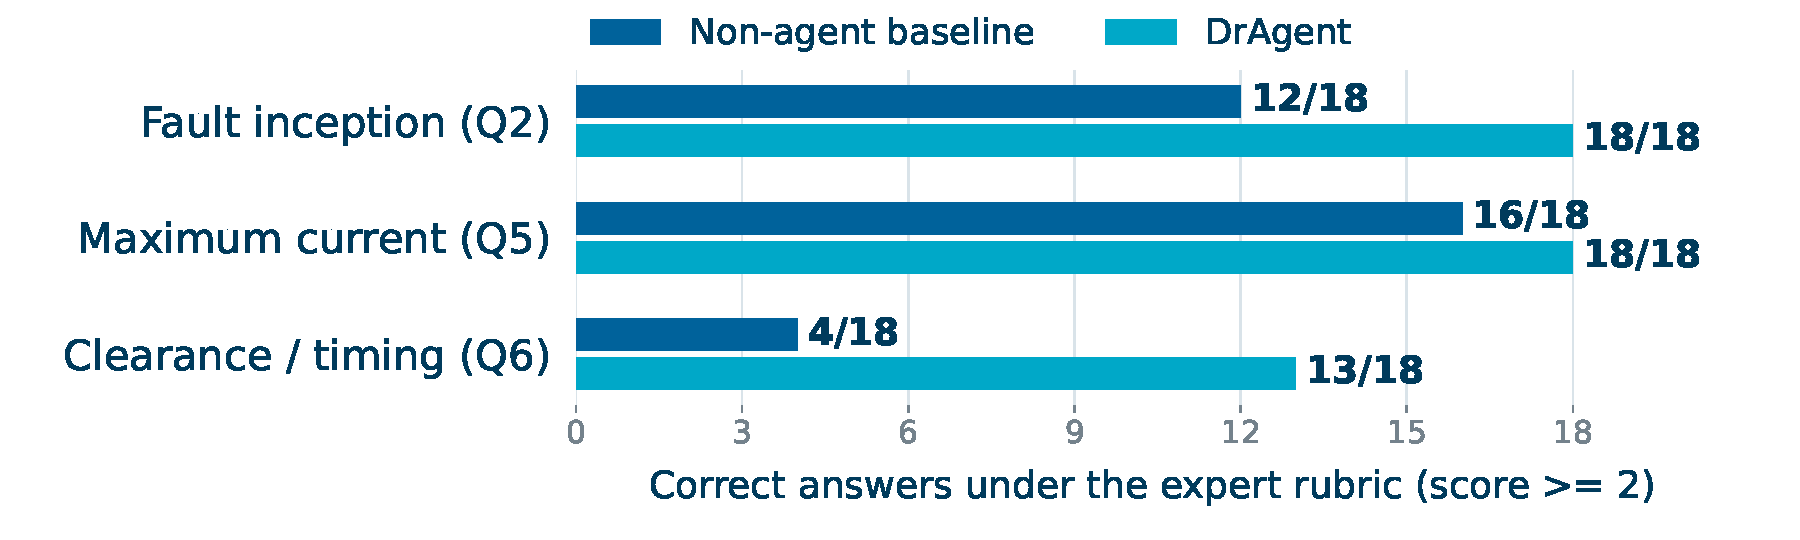
\includegraphics[width=\linewidth,height=3.65cm,keepaspectratio]{images/power_dragent_counts.pdf}
\par{\fontsize{7}{8.3}\selectfont\color{Slate} Counts reconstructed from Table IV and the Appendix. They are neither new experiments nor the paper's mean-score measure.}
\par\endgroup\smallskip
{
\small\begin{itemize}
\setlength{\itemsep}{.25em}
\item We counted scores of 2 or more as correct across the paper's 18 recorded cases.
\item Timing the fault's end remains harder. The grading rules also accept a correctly labeled fault duration.
\end{itemize}\par}
\vfill
{\fontsize{6.3}{7.5}\selectfont\color{Slate} Source: \href{https://www.manuscriptlink.com/society/kics/media?key=kics\%2Fconference\%2Ficaiic2025\%2Fpresentation\%2F1571098105.pdf}{Barun Kumar Saha, Aarthi V, O. D. Naidu. DrAgent: An Agentic Approach to Fault Analysis in Power Grids Using Large Language Models. 2025 International Conference on Artificial Intelligence in Information and Communication (ICAIIC), pp. 938--945. 2025-02-18--21.}\par}
\note{Fault inception: baseline 12/18, agent 18/18. Maximum current: baseline 16/18, agent 18/18. Clearance/timing: baseline 4/18, agent 13/18. The paper allows 3 ms timing error and 5\% current error. One expert graded the answers. Q6 footnote 8 accepts a correctly labeled duration, so these are not strictly clearance-timestamp accuracy counts. The printed Q6 mean conflicts with the individual cells. This chart therefore uses the audited cell counts. Takeaway: 

Barun Kumar Saha, Aarthi V, O. D. Naidu. DrAgent: An Agentic Approach to Fault Analysis in Power Grids Using Large Language Models. 2025 International Conference on Artificial Intelligence in Information and Communication (ICAIIC), pp. 938--945. 2025-02-18--21.
Full source: https://www.manuscriptlink.com/society/kics/media?key=kics\%2Fconference\%2Ficaiic2025\%2Fpresentation\%2F1571098105.pdf
Publication: https://doi.org/10.1109/ICAIIC64266.2025.10920654}
\end{frame}

\begin{frame}[t]{Three kinds of graph have different jobs}
\relax
\begingroup\begin{minipage}[c][3.8cm][c]{\linewidth}\centering\setbox0=\hbox{\resizebox{.96\linewidth}{!}{\begin{tikzpicture}[x=1cm,y=1cm,font=\sffamily\fontsize{12}{14}\selectfont,
  line cap=round,line join=round,
  rp/.style={circle,draw=rBlue,fill=white,minimum size=5.4mm,inner sep=0pt,line width=1.15pt},
  rl/.style={align=center,text=rNavy,font=\sffamily\bfseries\fontsize{12.5}{14.5}\selectfont},
  rn/.style={align=center,text=rNavy,font=\sffamily\fontsize{11.2}{13}\selectfont},
  rc/.style={align=left,text=rNavy,font=\ttfamily\fontsize{11}{13}\selectfont},
  rf/.style={-{Latex[length=2mm,width=1.5mm]},draw=rBlue,line width=1.15pt,shorten >=1.4pt,shorten <=1.4pt},
  rw/.style={-{Latex[length=2mm,width=1.5mm]},draw=rOrange,line width=1.15pt,shorten >=1.4pt,shorten <=1.4pt}]
\definecolor{rBlue}{HTML}{00629B}
\definecolor{rCyan}{HTML}{00A8C8}
\definecolor{rNavy}{HTML}{003B5C}
\definecolor{rOrange}{HTML}{B65B14}
\definecolor{rGray}{HTML}{74828C}
\path[use as bounding box] (0,0) rectangle (14.2,4.2);

\node[rl] at (2.25,3.85) {Grid connections};
\node[rl] at (7.0,3.85) {Task DAG};
\node[rl] at (11.8,3.85) {Workflow loop};
\node[rp] (b1) at (.85,2.25) {};
\node[rp] (b2) at (2.3,2.25) {};
\node[rp] (b3) at (3.75,2.25) {};
\node[rp] (b4) at (2.3,1.2) {};
\draw[draw=rBlue,line width=1.15pt] (b1.east) -- (b2.west);
\draw[draw=rBlue,line width=1.15pt] (b2.east) -- (b3.west);
\draw[draw=rBlue,line width=1.15pt] (b2.south) -- (b4.north);
\node[rn] at (.85,1.7) {B1};
\node[rn] at (2.3,2.88) {B2};
\node[rn] at (3.75,1.7) {B3};
\node[rn] at (2.3,.7) {B4};
\node[rn] at (2.25,.23) {equipment links};
\node[rp] (a) at (5.25,2.25) {};
\node[rp] (b) at (6.75,2.8) {};
\node[rp] (c) at (6.75,1.4) {};
\node[rp] (d) at (8.45,2.25) {};
\coordinate (fork) at (5.9,2.25);
\draw[draw=rBlue,line width=1.15pt] (a.east) -- (fork);
\draw[rf] (fork) |- (b.west);
\draw[rf] (fork) |- (c.west);
\coordinate (join) at (7.75,2.25);
\draw[draw=rBlue,line width=1.15pt] (b.east) -- (7.75,2.8) -- (join);
\draw[draw=rBlue,line width=1.15pt] (c.east) -- (7.75,1.4) -- (join);
\draw[rf] (join) -- (d.west);
\node[rn] at (5.25,1.7) {A};
\node[rn] at (6.75,3.28) {B};
\node[rn] at (6.75,.85) {C};
\node[rn] at (8.45,2.9) {D};
\node[rn] at (7.0,.23) {needed results};
\node[rp] (plan) at (10.15,2.25) {};
\node[rp] (tool) at (11.65,2.25) {};
\node[rp] (check) at (13.15,2.25) {};
\draw[rf] (plan.east) -- (tool.west);
\draw[rf] (tool.east) -- (check.west);
\node[rn] at (10.15,2.94) {Plan};
\node[rn] at (11.65,2.94) {Tool};
\node[rn] at (13.15,2.94) {Check};
\draw[rw] (check.south) -- (13.15,1.0) -- (10.15,1.0) -- (plan.south);
\node[rn,text=rOrange] at (11.65,1.38) {retry};
\node[rn] at (11.8,.23) {next software step};

\end{tikzpicture}
}}\ifdim\dimexpr\ht0+\dp0\relax>3.8cm\resizebox{!}{3.8cm}{\box0}\else\box0\fi\par\end{minipage}
{\fontsize{7}{8.3}\selectfont\color{Slate} Three different meanings of "graph." These small examples explain connections, not calculated electrical results.\par}
\endgroup\smallskip
{
\small\begin{itemize}
\setlength{\itemsep}{.25em}
\item Grid edges show electrical connections. A task DAG (directed acyclic graph) links calculations through the results they need.
\item Workflow edges show which software step can run next, including a retry loop.
\end{itemize}\par}
\vfill
{\fontsize{6.3}{7.5}\selectfont\color{Slate} Source: \href{https://www.manuscriptlink.com/society/kics/media?key=kics\%2Fconference\%2Ficaiic2025\%2Fpresentation\%2F1571098105.pdf}{Barun Kumar Saha, Aarthi V, O. D. Naidu. DrAgent: An Agentic Approach to Fault Analysis in Power Grids Using Large Language Models. 2025 International Conference on Artificial Intelligence in Information and Communication (ICAIIC), pp. 938--945. 2025-02-18--21.}\par}
\note{A radial feeder has a tree-like electrical layout, but its software can still contain loops. A calculation graph without loops can analyze a meshed electrical network. State which graph you mean before discussing a node, connection or loop. A software architecture drawing is not the electrical model. Takeaway: 

Barun Kumar Saha, Aarthi V, O. D. Naidu. DrAgent: An Agentic Approach to Fault Analysis in Power Grids Using Large Language Models. 2025 International Conference on Artificial Intelligence in Information and Communication (ICAIIC), pp. 938--945. 2025-02-18--21.
Full source: https://www.manuscriptlink.com/society/kics/media?key=kics\%2Fconference\%2Ficaiic2025\%2Fpresentation\%2F1571098105.pdf
Publication: https://doi.org/10.1109/ICAIIC64266.2025.10920654

D. Adrian Maldonado, Jonghwan Kwon, Sunash B. Sharma, Hongwei Jin, Stefano Fenu, Emil Constantinescu, David Sehloff, Parfait Gasana, Duane Rudolph Verner, Kibaek Kim. GridMind: An Agentic Workflow for Weather-Driven Power Grid Risk Assessment. KDD 2026 Workshop on Scientific and Societal Agents / OpenReview. August 2026 workshop; reviewed 17 October 2026.
Full source: https://openreview.net/forum?id=Cs5TBzzNym
Full paper: https://openreview.net/pdf/5ad1c2afd7298f9e6ce3bc25f18e7165555e1ffd.pdf

LangChain documentation maintainers. LangGraph Graph API overview. Official LangChain documentation. Accessed 2026-10-17; live documentation.
Full source: https://docs.langchain.com/oss/python/langgraph/graph-api}
\end{frame}

\begin{frame}[t]{A DAG shows which result must come first}
\relax
\begingroup\begin{minipage}[c][4cm][c]{\linewidth}\centering\setbox0=\hbox{\resizebox{.96\linewidth}{!}{\begin{tikzpicture}[x=1cm,y=1cm,font=\sffamily\fontsize{12}{14}\selectfont,
  line cap=round,line join=round,
  rp/.style={circle,draw=rBlue,fill=white,minimum size=5.4mm,inner sep=0pt,line width=1.15pt},
  rl/.style={align=center,text=rNavy,font=\sffamily\bfseries\fontsize{12.5}{14.5}\selectfont},
  rn/.style={align=center,text=rNavy,font=\sffamily\fontsize{11.2}{13}\selectfont},
  rc/.style={align=left,text=rNavy,font=\ttfamily\fontsize{11}{13}\selectfont},
  rf/.style={-{Latex[length=2mm,width=1.5mm]},draw=rBlue,line width=1.15pt,shorten >=1.4pt,shorten <=1.4pt},
  rw/.style={-{Latex[length=2mm,width=1.5mm]},draw=rOrange,line width=1.15pt,shorten >=1.4pt,shorten <=1.4pt}]
\definecolor{rBlue}{HTML}{00629B}
\definecolor{rCyan}{HTML}{00A8C8}
\definecolor{rNavy}{HTML}{003B5C}
\definecolor{rOrange}{HTML}{B65B14}
\definecolor{rGray}{HTML}{74828C}
\path[use as bounding box] (0,0) rectangle (14.2,4.2);

\node[rp] (record) at (1.35,2.05) {};
\node[rl] at (1.35,3.05) {Frozen\\R17};
\node[rn] at (1.35,1.45) {.cfg + .dat};
\coordinate (fork) at (2.45,2.05);
\draw[rf] (record.east) -- (fork);
\fill[rBlue] (fork) circle (1.8pt);
\node[rp] (inception) at (4.75,3.2) {};
\node[rl] at (4.75,3.85) {Find inception};
\node[rn] at (4.75,2.7) {sample n\textsubscript{f}};
\draw[rf] (fork) |- (inception.west);
\node[rp] (maximum) at (4.75,.95) {};
\node[rl] at (4.75,1.52) {Find max current};
\node[rn] at (4.75,.45) {I\textsubscript{max}};
\draw[rf] (fork) |- (maximum.west);
\node[rp] (rate) at (8.55,2.05) {};
\node[rn] at (8.55,1.5) {CFG: rate f\textsubscript{s}};
\draw[rf] (fork) -- (rate.west);
\node[rp] (time) at (8.55,3.2) {};
\node[rl] at (8.55,3.85) {Convert to time};
\node[rn] at (6.65,3.6) {n\textsubscript{f}};
\node[rn] at (9.75,2.65) {n\textsubscript{f} / f\textsubscript{s}};
\draw[rf] (inception.east) -- (time.west);
\draw[rf] (rate.north) -- (time.south);
\coordinate (join) at (11.05,2.05);
\draw[rf] (time.east) -- (11.05,3.2) -- (join);
\draw[rf] (maximum.east) -- (11.05,.95) -- (join);
\fill[rBlue] (join) circle (2pt);
\node[rp] (report) at (13.0,2.05) {};
\draw[rf] (join) -- (report.west);
\node[rl] at (13.0,2.85) {Report};
\node[rn] at (13.0,1.45) {evidence};

\end{tikzpicture}
}}\ifdim\dimexpr\ht0+\dp0\relax>4cm\resizebox{!}{4cm}{\box0}\else\box0\fi\par\end{minipage}
{\fontsize{7}{8.3}\selectfont\color{Slate} Original teaching adaptation of DrAgent's tool dependencies, rather than its exact execution graph.\par}
\endgroup\smallskip
{
\small\begin{itemize}
\setlength{\itemsep}{.25em}
\item A DAG links results to calculations that need them. Its arrows do not form a loop.
\item Run independent calculations when inputs are ready. Wait for every required result before reporting.
\end{itemize}\par}
\vfill
{\fontsize{6.3}{7.5}\selectfont\color{Slate} Source: \href{https://www.manuscriptlink.com/society/kics/media?key=kics\%2Fconference\%2Ficaiic2025\%2Fpresentation\%2F1571098105.pdf}{Barun Kumar Saha, Aarthi V, O. D. Naidu. DrAgent: An Agentic Approach to Fault Analysis in Power Grids Using Large Language Models. 2025 International Conference on Artificial Intelligence in Information and Communication (ICAIIC), pp. 938--945. 2025-02-18--21.}\par}
\note{Every task must follow the tasks that produce its inputs. This is a valid topological order. Fault-start sample and sampling rate must both exist before the time conversion runs. Finding maximum current can run independently of that conversion when both use the same unchanged record. Dependencies determine which tasks can run together. The positions of boxes in a drawing do not. Takeaway: 

Barun Kumar Saha, Aarthi V, O. D. Naidu. DrAgent: An Agentic Approach to Fault Analysis in Power Grids Using Large Language Models. 2025 International Conference on Artificial Intelligence in Information and Communication (ICAIIC), pp. 938--945. 2025-02-18--21.
Full source: https://www.manuscriptlink.com/society/kics/media?key=kics\%2Fconference\%2Ficaiic2025\%2Fpresentation\%2F1571098105.pdf
Publication: https://doi.org/10.1109/ICAIIC64266.2025.10920654}
\end{frame}

\begin{frame}[t]{LangGraph can pause to inspect a run}
\relax
\begin{columns}[T,onlytextwidth]\begin{column}{.64\textwidth}
\begingroup\centering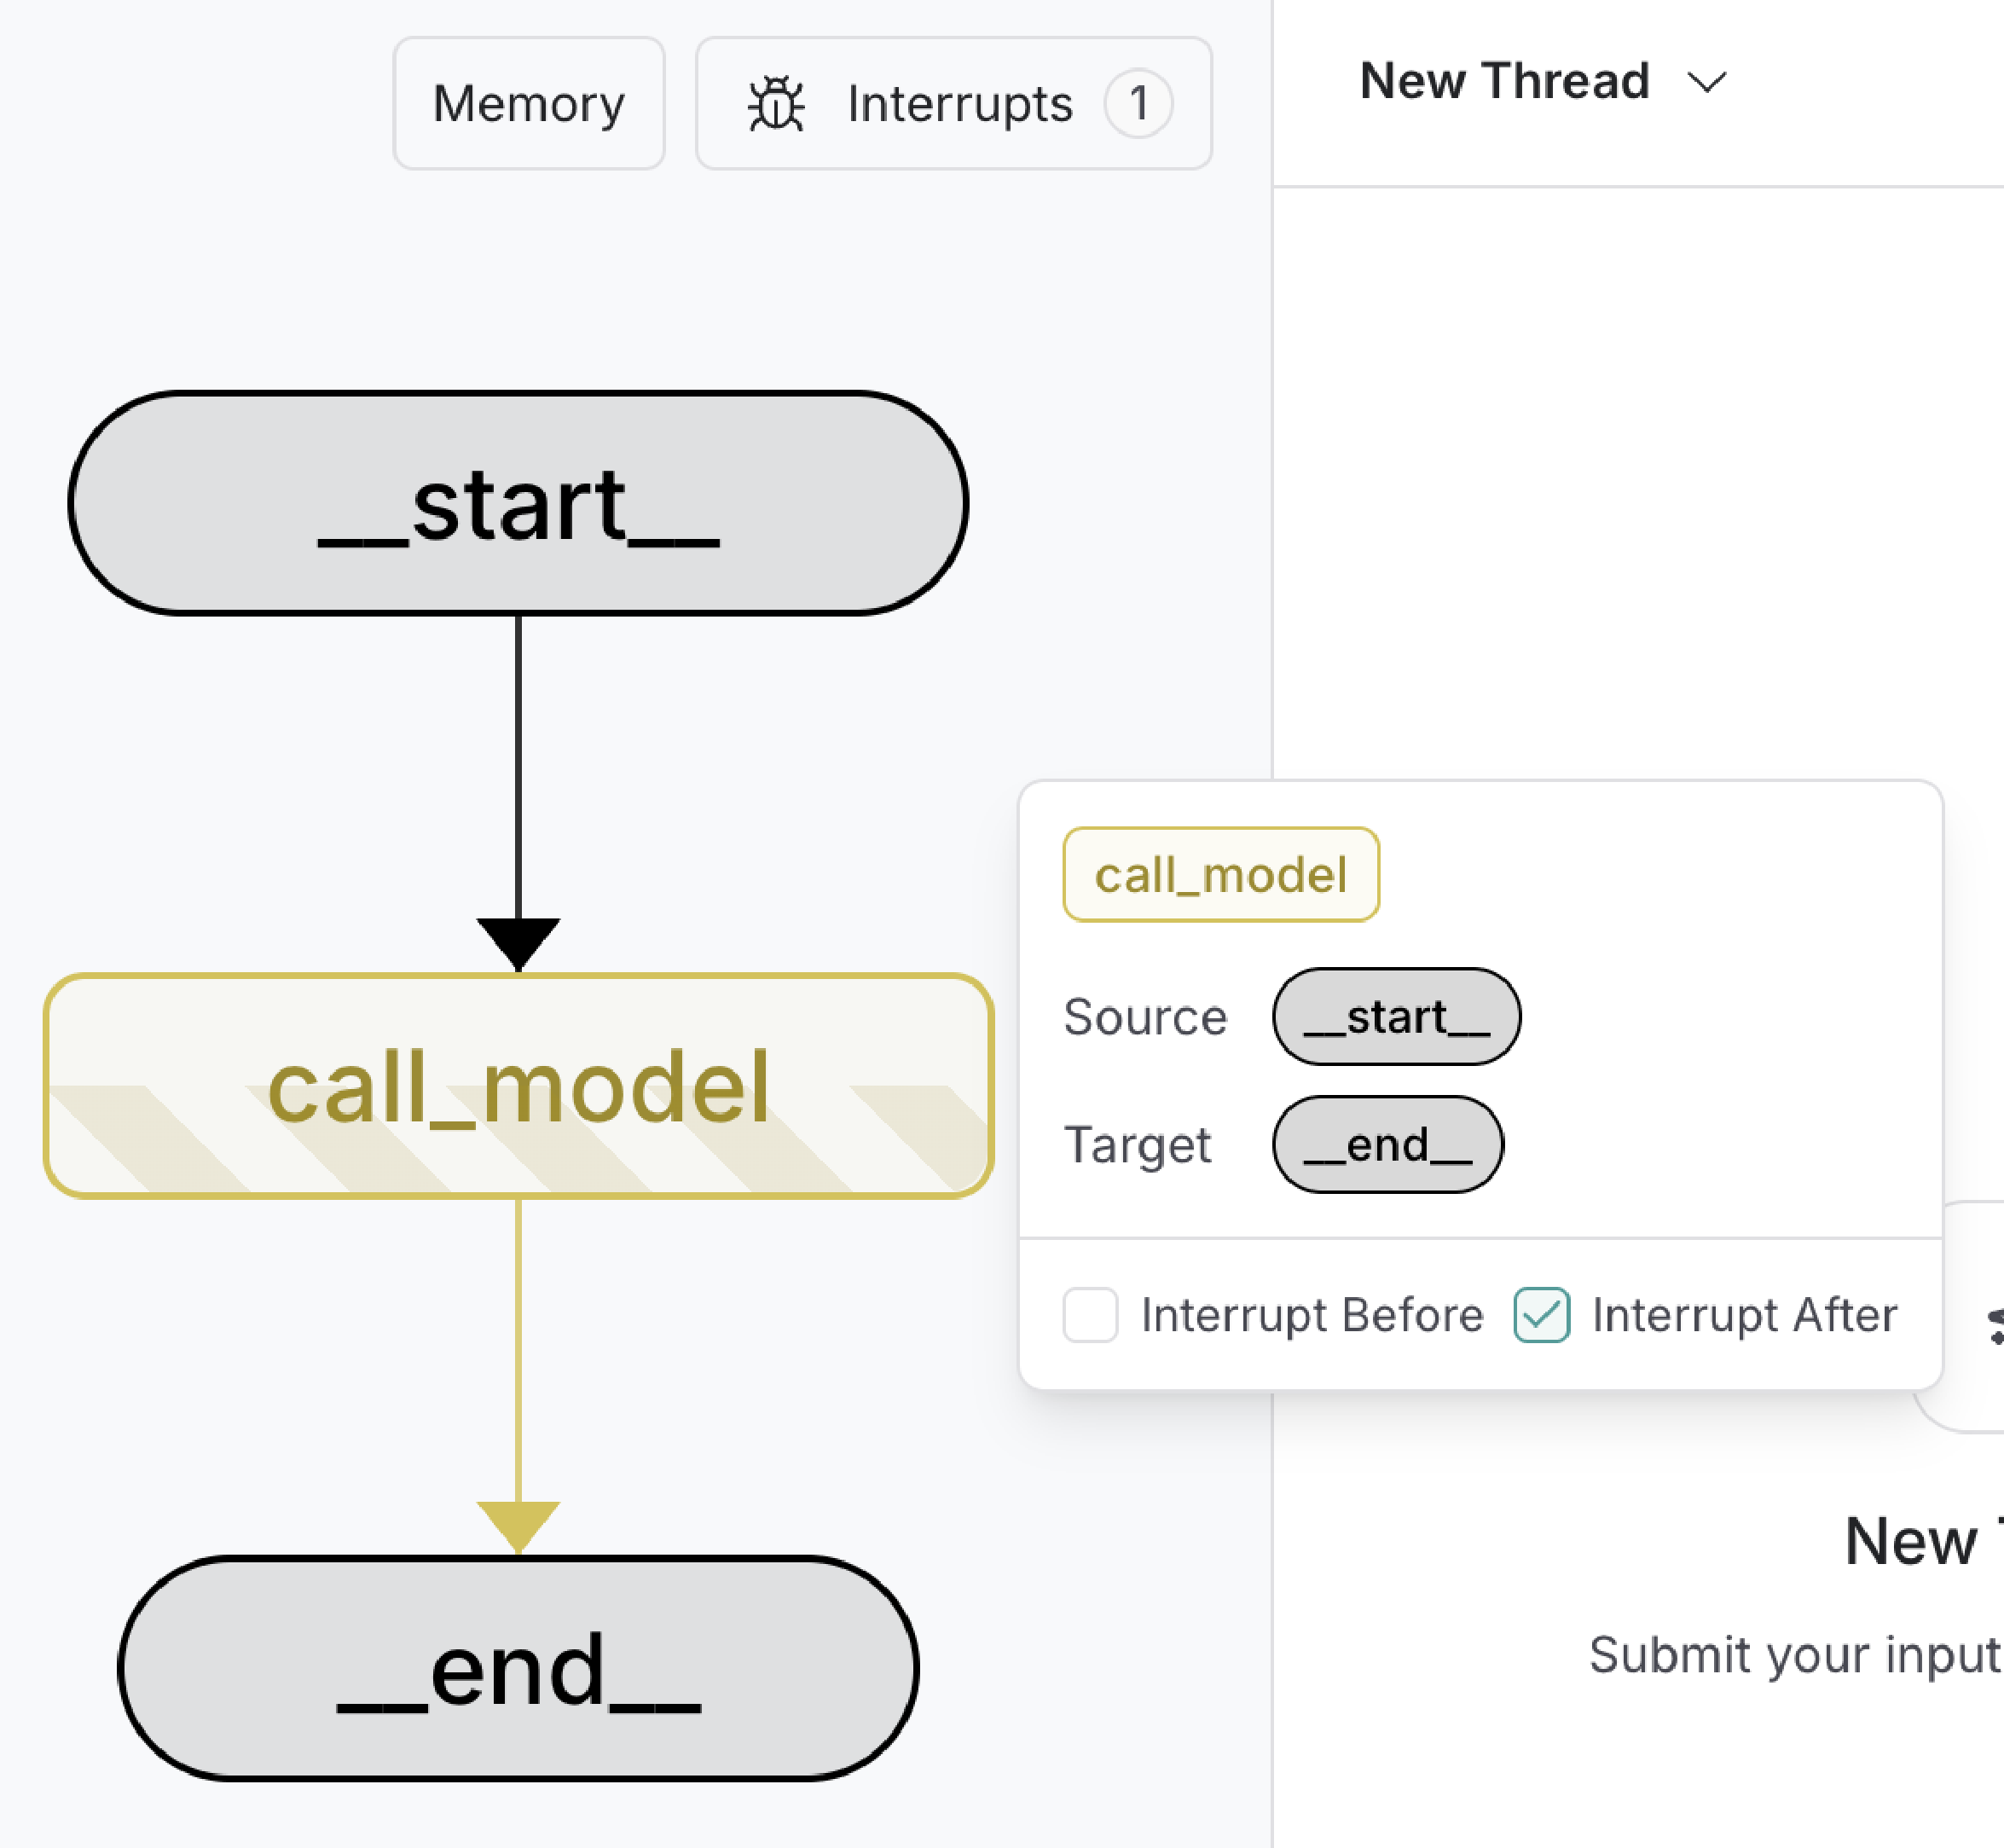
\includegraphics[width=\linewidth,height=4.65cm,keepaspectratio]{images/real_framework_langgraph_static_interrupt.pdf}
\par{\fontsize{7}{8.3}\selectfont\color{Slate} Real LangGraph debugger screenshot. A paused run can be inspected before the next software step.}
\par\endgroup\smallskip
\end{column}\begin{column}{.32\textwidth}
{
\small\begin{itemize}
\setlength{\itemsep}{.25em}
\item A debugger can pause the graph so a developer can inspect it. A failed check can also send execution back to an earlier step.
\item Software routing does not check the grid model. The application still checks inputs and engineering results.
\end{itemize}\par}
\end{column}\end{columns}
\vfill
{\fontsize{6.3}{7.5}\selectfont\color{Slate} Source: \href{https://docs.langchain.com/oss/python/langgraph/graph-api}{LangChain documentation maintainers. LangGraph Graph API overview. Official LangChain documentation. Accessed 2026-10-17; live documentation.}\par}
\note{LangGraph is software for running workflows. It can support loops, unlike a DAG. StateGraph defines stored state fields and workflow nodes. Application-defined reducers specify how updates from parallel steps combine. A node may call an engineering tool with fixed rules or an AI model. The application must define validation, stopping and permissions. Running the graph does not prove that an electrical solution is feasible. Source: LangChain documentation maintainers, official LangGraph documentation. Accessed October 18, 2026. A static debug breakpoint differs from a dynamic interrupt requesting human input. Source figure locator: Debugging with interrupts. Original source URL: https://docs.langchain.com/oss/python/langgraph/interrupts Takeaway: 

LangChain documentation maintainers. LangGraph Graph API overview. Official LangChain documentation. Accessed 2026-10-17; live documentation.
Full source: https://docs.langchain.com/oss/python/langgraph/graph-api

Barun Kumar Saha, Aarthi V, O. D. Naidu. DrAgent: An Agentic Approach to Fault Analysis in Power Grids Using Large Language Models. 2025 International Conference on Artificial Intelligence in Information and Communication (ICAIIC), pp. 938--945. 2025-02-18--21.
Full source: https://www.manuscriptlink.com/society/kics/media?key=kics\%2Fconference\%2Ficaiic2025\%2Fpresentation\%2F1571098105.pdf
Publication: https://doi.org/10.1109/ICAIIC64266.2025.10920654

D. Adrian Maldonado, Jonghwan Kwon, Sunash B. Sharma, Hongwei Jin, Stefano Fenu, Emil Constantinescu, David Sehloff, Parfait Gasana, Duane Rudolph Verner, Kibaek Kim. GridMind: An Agentic Workflow for Weather-Driven Power Grid Risk Assessment. KDD 2026 Workshop on Scientific and Societal Agents / OpenReview. August 2026 workshop; reviewed 17 October 2026.
Full source: https://openreview.net/forum?id=Cs5TBzzNym
Full paper: https://openreview.net/pdf/5ad1c2afd7298f9e6ce3bc25f18e7165555e1ffd.pdf

LangChain documentation maintainers. LangGraph Interrupts. Official LangChain documentation. Accessed 2026-10-17; live documentation.
Full source: https://docs.langchain.com/oss/python/langgraph/interrupts}
\end{frame}

\begin{frame}[t]{Saved state must identify the study and its evidence}
\relax
\begingroup\centering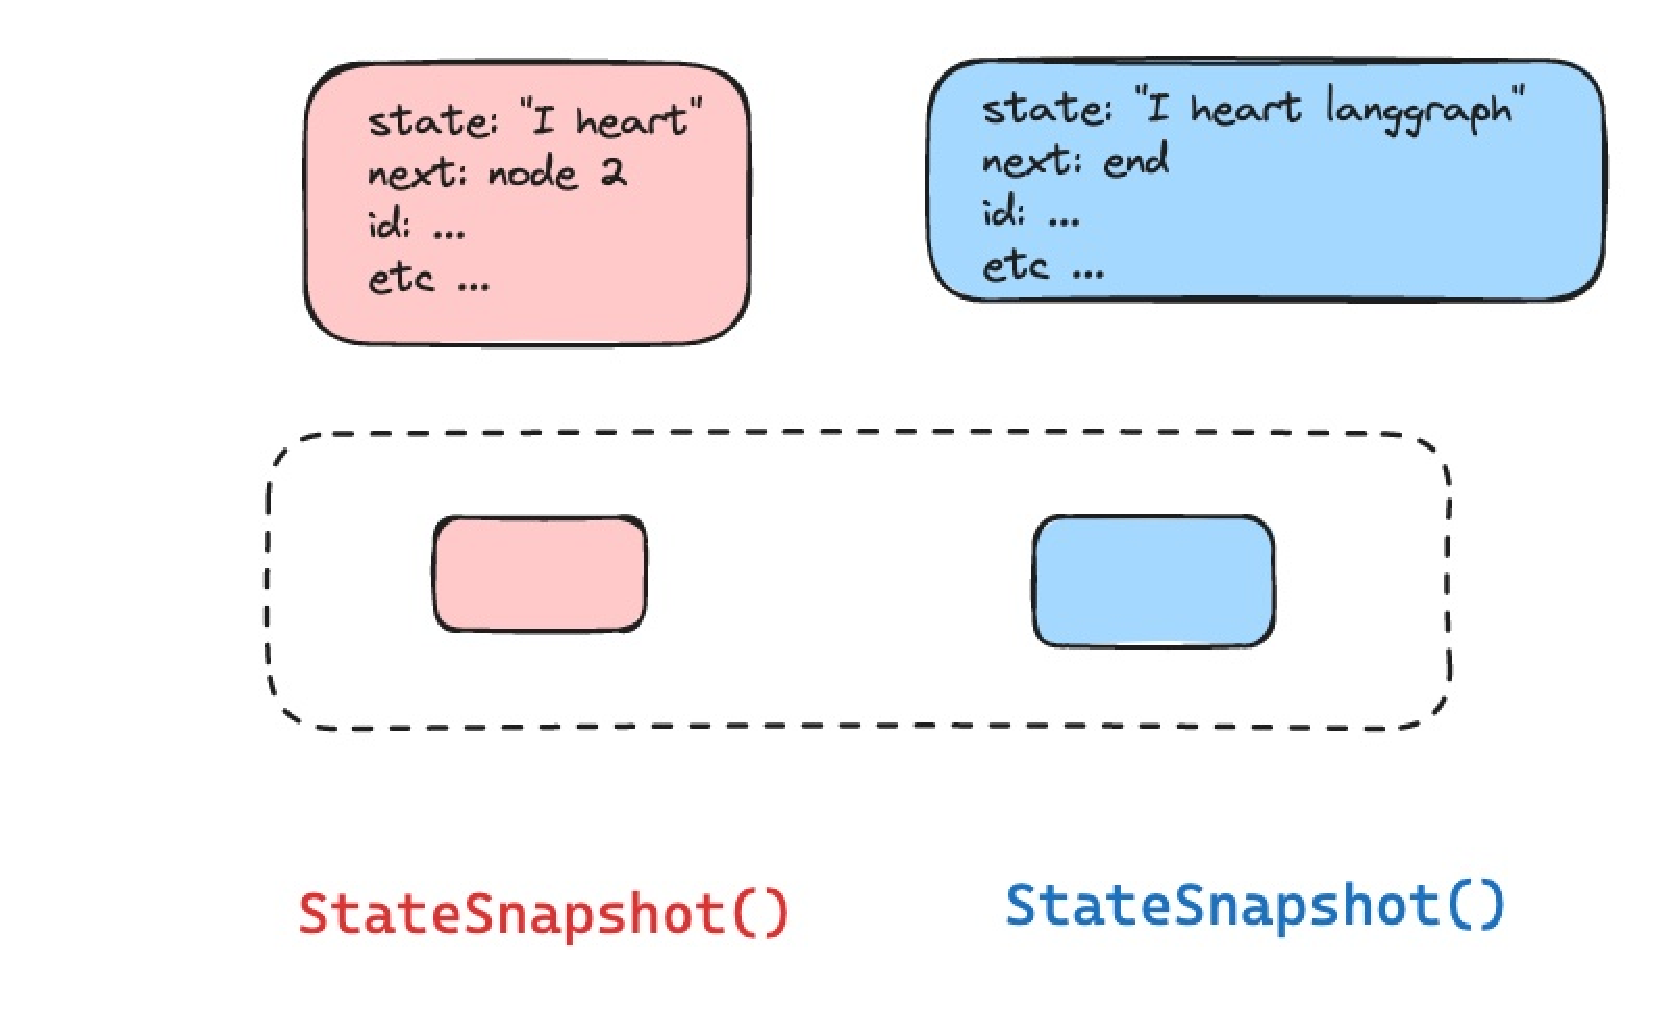
\includegraphics[width=\linewidth,height=3.7cm,keepaspectratio]{images/real_framework_langgraph_state.pdf}
\par{\fontsize{7}{8.3}\selectfont\color{Slate} Original LangGraph state diagram. Software checkpoints still need grid-case, time and evidence identifiers.}
\par\endgroup\smallskip
{
\small\begin{itemize}
\setlength{\itemsep}{.25em}
\item Save the case ID, input versions, evidence, status and attempt count.
\item Label each result with its case or outage ID. This helps reveal missing or duplicate results when parallel work comes together.
\end{itemize}\par}
\vfill
{\fontsize{6.3}{7.5}\selectfont\color{Slate} Source: \href{https://docs.langchain.com/oss/python/langgraph/graph-api}{LangChain documentation maintainers. LangGraph Graph API overview. Official LangChain documentation. Accessed 2026-10-17; live documentation.}\par}
\note{The published figure shows generic LangGraph software state. For a spoken grid-study example, imagine an application-specific expected-case set that includes outage\_34 while the returned evidence lacks that case. Those case fields are tutorial requirements, not a built-in LangGraph power-system schema. Default update behavior does not guarantee that all branch results survive a merge. Define and test the reducer, or an external evidence store, to preserve case IDs and detect duplicates or missing outputs. Source: LangChain documentation maintainers, official LangGraph documentation. Accessed October 18, 2026. The extra grid identifiers are tutorial requirements; they are not fields proven by this generic illustration. Source figure locator: Get state history. Original source URL: https://docs.langchain.com/oss/python/langgraph/checkpointers Takeaway: Saved state identifies the evidence. The application still has to check it.

LangChain documentation maintainers. LangGraph Graph API overview. Official LangChain documentation. Accessed 2026-10-17; live documentation.
Full source: https://docs.langchain.com/oss/python/langgraph/graph-api

LangChain documentation maintainers. LangGraph Persistence. Official LangChain documentation. Accessed 2026-10-17; live documentation.
Full source: https://docs.langchain.com/oss/python/langgraph/persistence

LangChain documentation maintainers. Checkpointers. Docs by LangChain, Python LangGraph documentation. Undated live documentation; accessed October 18, 2026.
Full source: https://docs.langchain.com/oss/python/langgraph/checkpointers}
\end{frame}

\begin{frame}[t]{A checkpoint lets a workflow pause and resume}
\relax
\begingroup\centering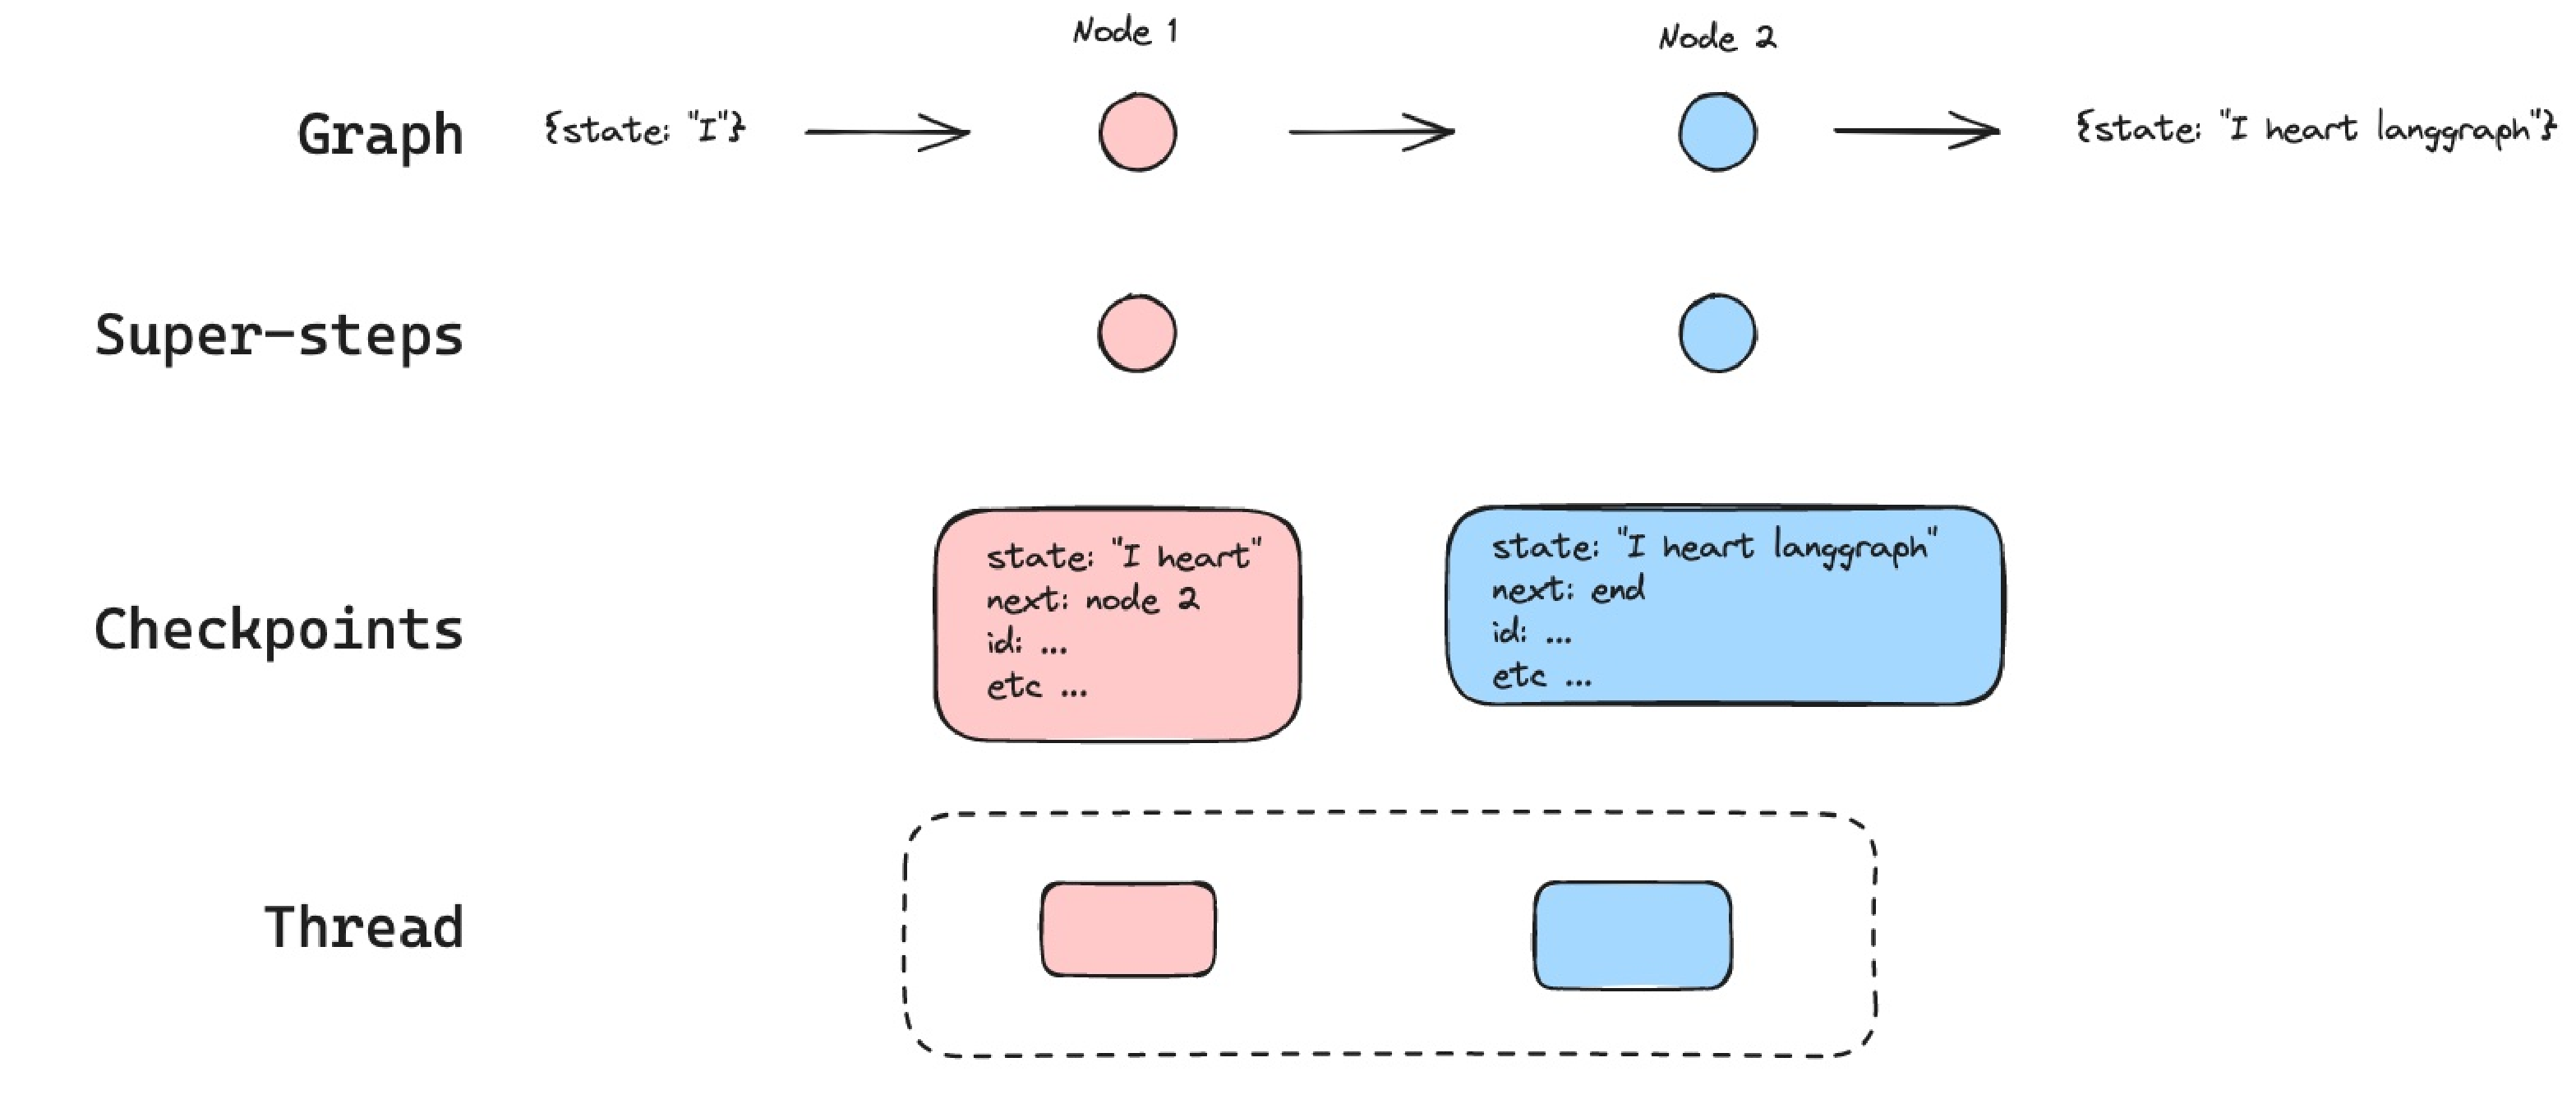
\includegraphics[width=\linewidth,height=3.7cm,keepaspectratio]{images/real_framework_langgraph_checkpoint.pdf}
\par{\fontsize{7}{8.3}\selectfont\color{Slate} Original LangGraph checkpoint diagram. Saving progress does not prove that the grid data still match.}
\par\endgroup\smallskip
{
\small\begin{itemize}
\setlength{\itemsep}{.25em}
\item A checkpoint saves progress; thread\_id links the saved steps to the same workflow.
\item Changed grid connections can make old results invalid. Check them and rerun affected studies.
\end{itemize}\par}
\vfill
{\fontsize{6.3}{7.5}\selectfont\color{Slate} Source: \href{https://docs.langchain.com/oss/python/langgraph/persistence}{LangChain documentation maintainers. LangGraph Persistence. Official LangChain documentation. Accessed 2026-10-17; live documentation.}\par}
\note{An interrupt can pause for outside review and later resume in the same thread. Current LangGraph documentation says the interrupted node restarts from its beginning. Actions before the interrupt can therefore happen again. Use stable step IDs or other idempotency controls, which prevent repeated execution from applying the same change twice. This example grants no permission to command live grid equipment. Source: LangChain documentation maintainers, official LangGraph documentation. Accessed October 18, 2026. Saved software state does not prove that an external grid snapshot remains current. Source figure locator: Opening checkpoint illustration. Original source URL: https://docs.langchain.com/oss/python/langgraph/checkpointers Takeaway: 

LangChain documentation maintainers. LangGraph Persistence. Official LangChain documentation. Accessed 2026-10-17; live documentation.
Full source: https://docs.langchain.com/oss/python/langgraph/persistence

LangChain documentation maintainers. LangGraph Interrupts. Official LangChain documentation. Accessed 2026-10-17; live documentation.
Full source: https://docs.langchain.com/oss/python/langgraph/interrupts

LangChain documentation maintainers. Checkpointers. Docs by LangChain, Python LangGraph documentation. Undated live documentation; accessed October 18, 2026.
Full source: https://docs.langchain.com/oss/python/langgraph/checkpointers}
\end{frame}

\begin{frame}[t]{Parallel outage studies must account for every case}
\relax
\begingroup\centering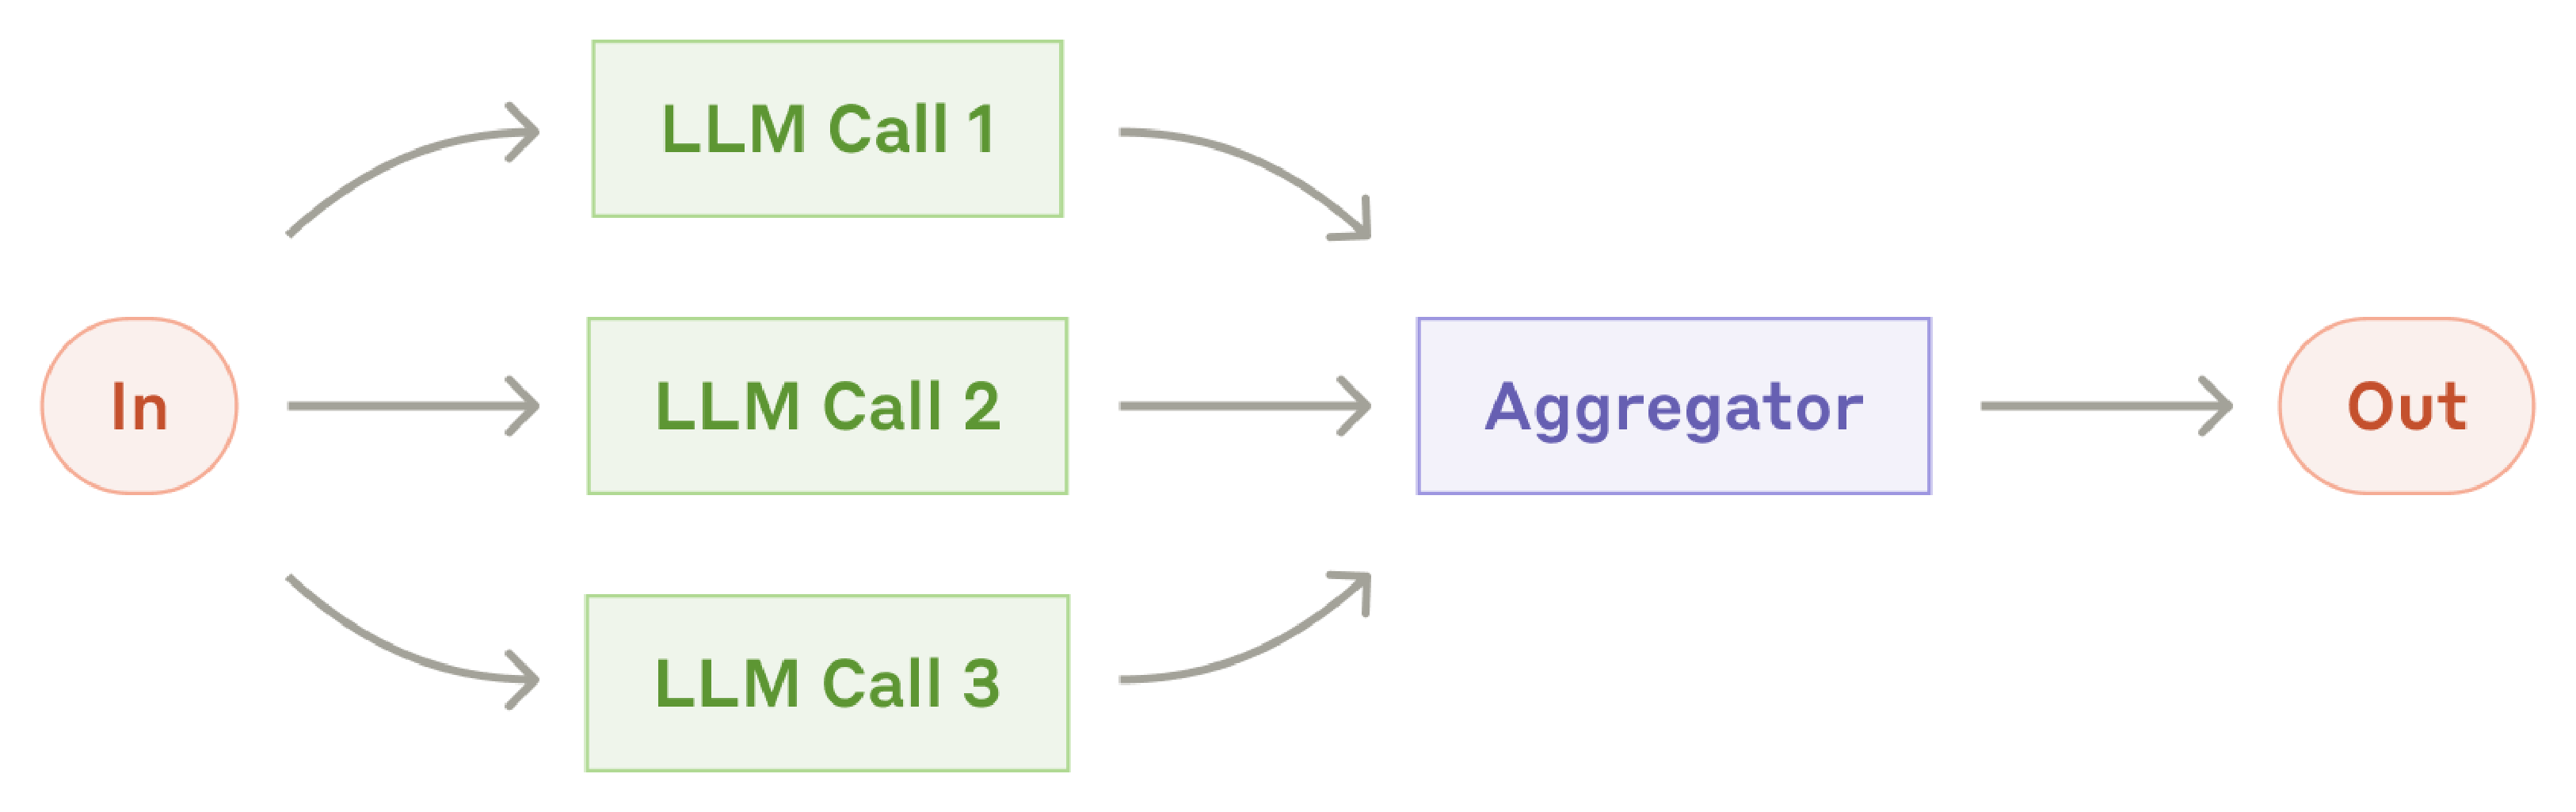
\includegraphics[width=\linewidth,height=3.7cm,keepaspectratio]{images/real_framework_anthropic_parallel.pdf}
\par{\fontsize{7}{8.3}\selectfont\color{Slate} Original Anthropic parallel workflow. A grid study must also account for missing or failed outage cases.}
\par\endgroup\smallskip
{
\small\begin{itemize}
\setlength{\itemsep}{.25em}
\item Run each selected outage on a separate, consistent copy of the same starting grid case.
\item Before combining results, compare the returned case IDs with the expected list. Mark failed or missing cases as unresolved.
\end{itemize}\par}
\vfill
{\fontsize{6.3}{7.5}\selectfont\color{Slate} Source: \href{https://arxiv.org/pdf/2512.20789v1}{Yihan (Logon) Wen, Xin Chen. X-GridAgent: An LLM-Powered Agentic AI System for Assisting Power Grid Analysis. arXiv preprint. 2025-12-23 (v1).}\par}
\note{The goal is complete evidence for the selected study scope, rather than a count of completed software steps. In a spoken grid-study example, if a case named C2 fails, the output should name C2, explain its failure and state what remains unknown. This applies AgentiGrid's lesson about incomplete coverage. Completing a selected set of outages does not prove coverage of every N-1 contingency, meaning every relevant single-component outage. Source: Anthropic, Building effective agents (December 19, 2024). The aggregator picture does not imply that missing results are automatically detected. Source figure locator: Workflow: Parallelization. Original source URL: https://www.anthropic.com/engineering/building-effective-agents Takeaway: 

Yihan (Logon) Wen, Xin Chen. X-GridAgent: An LLM-Powered Agentic AI System for Assisting Power Grid Analysis. arXiv preprint. 2025-12-23 (v1).
Full source: https://arxiv.org/pdf/2512.20789v1

Samim Konjicija, Slaven Peles. Integrating Agentic Artificial Intelligence with High-Performance Computing for Grid Planning. arXiv; EnergyCon 2026 proceedings forthcoming as described by authors. 3 September 2026; v1.
Full source: https://arxiv.org/abs/2609.04544v1
Full paper: https://arxiv.org/pdf/2609.04544v1

LangChain documentation maintainers. LangGraph Graph API overview. Official LangChain documentation. Accessed 2026-10-17; live documentation.
Full source: https://docs.langchain.com/oss/python/langgraph/graph-api

Erik S., Barry Zhang. Building effective agents. Anthropic Engineering. 2024-12-19.
Full source: https://www.anthropic.com/engineering/building-effective-agents}
\end{frame}

\begin{frame}[t]{PowerDAG checks the steps needed before a tool runs}
\relax
\begin{columns}[T,onlytextwidth]\begin{column}{.64\textwidth}
\begingroup\centering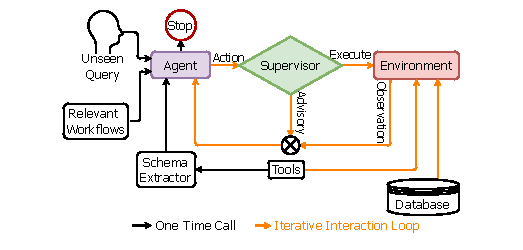
\includegraphics[width=\linewidth,height=4.6cm,keepaspectratio]{images/real_paper_powerdag_architecture.pdf}
\par{\fontsize{7}{8.3}\selectfont\color{Slate} Original PowerDAG v4 architecture, including the supervisor before environment execution.}
\par\endgroup\smallskip
\end{column}\begin{column}{.32\textwidth}
{
\small\begin{itemize}
\setlength{\itemsep}{.25em}
\item PowerDAG finds relevant verified workflow examples. It uses a dependency graph and a gate that checks required earlier tool calls.
\item The benchmark covers 108 tools, ten task families and four Vermont feeder models (local distribution networks).
\end{itemize}\par}
\end{column}\end{columns}
\vfill
{\fontsize{6.3}{7.5}\selectfont\color{Slate} Source: \href{https://arxiv.org/pdf/2603.17418v4}{Emmanuel O. Badmus, Amritanshu Pandey. PowerDAG: Supervisory Agentic AI System for Automating Distribution Grid Analysis. arXiv preprint, version 4. 5 July 2026 (v4); first submitted 18 March 2026.}\par}
\note{Use the inspected v4 dated 5 July 2026: Emmanuel O. Badmus and Amritanshu Pandey, PowerDAG: Supervisory Agentic AI System for Automating Distribution Grid Analysis. Earlier versions have different titles and performance headlines. Its four network models are Rochester, Stowe, Glover and South Hero. The graph identifies required earlier tools and gates calls while the agent continues choosing steps. A tool can run successfully in the wrong study state if earlier work is missing. The gate addresses that workflow problem. Emmanuel O. Badmus, Amritanshu Pandey; PowerDAG: Supervisory Agentic AI System for Automating Distribution Grid Analysis; Figure 2, v4 PDF page 3 This is the v4 research architecture. Formal supervision checks encoded prior Write-tool names; it does not establish all freshness, parameter or physical-safety checks. Source locator: Figure 2, v4 PDF page 3. Original URL: https://arxiv.org/pdf/2603.17418v4 Takeaway: 

Emmanuel O. Badmus, Amritanshu Pandey. PowerDAG: Supervisory Agentic AI System for Automating Distribution Grid Analysis. arXiv preprint, version 4. 5 July 2026 (v4); first submitted 18 March 2026.
Full source: https://arxiv.org/pdf/2603.17418v4

Emmanuel O. Badmus and contributors. DistGrid-AgentBench: A Distribution Grid Benchmark for Agentic AI. Author-maintained GitHub repository. Live repository reviewed 17 October 2026.
Full source: https://github.com/emmanuelbadmus/DistGrid-AgentBench}
\end{frame}

\begin{frame}[t]{PowerDAG: solve the grid before checking its voltage}
\relax
\begingroup\begin{minipage}[c][4cm][c]{\linewidth}\centering\setbox0=\hbox{\resizebox{.96\linewidth}{!}{\begin{tikzpicture}[x=1cm,y=1cm,font=\sffamily\fontsize{12}{14}\selectfont,
  line cap=round,line join=round,
  rp/.style={circle,draw=rBlue,fill=white,minimum size=5.4mm,inner sep=0pt,line width=1.15pt},
  rl/.style={align=center,text=rNavy,font=\sffamily\bfseries\fontsize{12.5}{14.5}\selectfont},
  rn/.style={align=center,text=rNavy,font=\sffamily\fontsize{11.2}{13}\selectfont},
  rc/.style={align=left,text=rNavy,font=\ttfamily\fontsize{11}{13}\selectfont},
  rf/.style={-{Latex[length=2mm,width=1.5mm]},draw=rBlue,line width=1.15pt,shorten >=1.4pt,shorten <=1.4pt},
  rw/.style={-{Latex[length=2mm,width=1.5mm]},draw=rOrange,line width=1.15pt,shorten >=1.4pt,shorten <=1.4pt}]
\definecolor{rBlue}{HTML}{00629B}
\definecolor{rCyan}{HTML}{00A8C8}
\definecolor{rNavy}{HTML}{003B5C}
\definecolor{rOrange}{HTML}{B65B14}
\definecolor{rGray}{HTML}{74828C}
\path[use as bounding box] (0,0) rectangle (14.2,4.2);

\node[rp] (planner) at (1.5,2.5) {};
\node[rl] at (1.5,3.25) {Planner};
\node[rp] (gate) at (7.0,2.5) {};
\node[rl] at (7.0,3.5) {Gate:\\solved for v43?};
\node[rp] (check) at (11.95,2.5) {};
\node[rl] at (11.95,3.4) {Run voltage\\check};
\node[rn] at (11.95,1.87) {current solution};
\draw[rf] (planner.east) -- (gate.west);
\node[rn] at (4.0,2.96) {propose check};
\draw[rf] (gate.east) -- (check.west);
\node[rn] at (9.45,2.96) {met};
\draw[rw] (gate.south) -- (7.0,.78) -- (1.5,.78) -- (planner.south);
\node[rn,text=rOrange,anchor=west] at (7.35,1.52) {unmet: no execution};
\node[rn,text=rOrange] at (4.25,1.2) {missing: solve v43 first};

\end{tikzpicture}
}}\ifdim\dimexpr\ht0+\dp0\relax>4cm\resizebox{!}{4cm}{\box0}\else\box0\fi\par\end{minipage}
{\fontsize{7}{8.3}\selectfont\color{Slate} Teaching adaptation: the current-v43 check adds a freshness rule. The paper's gate checks which required tools have already run.\par}
\endgroup\smallskip
{
\small\begin{itemize}
\setlength{\itemsep}{.25em}
\item In the paper's example, a voltage-violation check needs a solved network state first.
\item If an earlier required step is missing, the gate rejects the call and tells the agent what to do first.
\end{itemize}\par}
\vfill
{\fontsize{6.3}{7.5}\selectfont\color{Slate} Source: \href{https://arxiv.org/pdf/2603.17418v4}{Emmanuel O. Badmus, Amritanshu Pandey. PowerDAG: Supervisory Agentic AI System for Automating Distribution Grid Analysis. arXiv preprint, version 4. 5 July 2026 (v4); first submitted 18 March 2026.}\par}
\note{Section IV-C uses voltage-violation checks to explain these requirements. Equation 9 checks whether required Write-tool names appear among executed tool names. That alone does not check whether their outputs match the current grid version. The diagram adds current-v43 freshness as a teaching condition. The introduction also explains how missing a network update can leave a solver using the wrong state. Appendix B reports this Stowe execution order: load\_load, load\_solar, load\_distribution\_network, create\_and\_initialize\_model, build\_constraints, build\_objective, solve, update\_network\_voltages and plot\_network\_data. This is a reported order, not a claimed minimal set of dependency links. The authors curate the rules. Tools without rules remain executable. Passing the gate does not prove numerical feasibility or safety. Takeaway: 

Emmanuel O. Badmus, Amritanshu Pandey. PowerDAG: Supervisory Agentic AI System for Automating Distribution Grid Analysis. arXiv preprint, version 4. 5 July 2026 (v4); first submitted 18 March 2026.
Full source: https://arxiv.org/pdf/2603.17418v4}
\end{frame}

\begin{frame}[t]{PowerDAG results: the same queries, four setups}
\relax
\begingroup\centering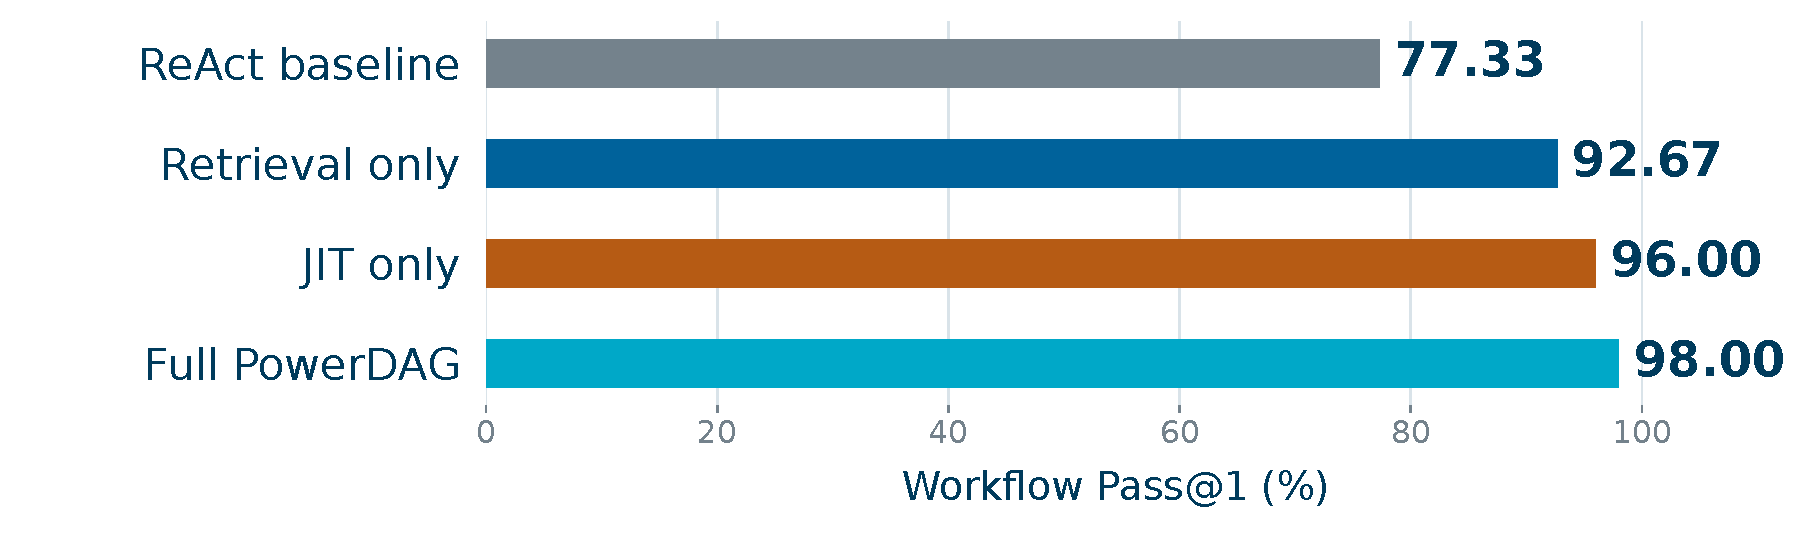
\includegraphics[width=\linewidth,height=3.55cm,keepaspectratio]{images/powerdag_revision_result.pdf}
\par{\fontsize{7}{8.3}\selectfont\color{Slate} PowerDAG v4, Table II. ReAct: a reason-and-act loop. JIT: prerequisite checks just before a call.}
\par\endgroup\smallskip
{
\small\begin{itemize}
\setlength{\itemsep}{.25em}
\item Each GPT-5.5 setup runs the same 150 test queries once.
\item Pass@1 measures first-run workflow success: required tool calls, valid inputs and correct order. It does not measure field reliability.
\end{itemize}\par}
\vfill
{\fontsize{6.3}{7.5}\selectfont\color{Slate} Source: \href{https://arxiv.org/pdf/2603.17418v4}{Emmanuel O. Badmus, Amritanshu Pandey. PowerDAG: Supervisory Agentic AI System for Automating Distribution Grid Analysis. arXiv preprint, version 4. 5 July 2026 (v4); first submitted 18 March 2026.}\par}
\note{The reported Pass@1 scores are ReAct 77.33\%, retrieval-only PowerChain-AR 92.67\%, JIT supervision only 96.00\%, and full PowerDAG 98.00\%. Each setup runs 150 queries. Across the full study, six setups and ten model backends produce 9,000 query runs. Full PowerDAG scores 97.33\% with Gemini 3.1 Pro and 92.67\% with Qwen 3.6-27B. Pass@1 is an automated check against expert workflows. The test queries were kept out of the example set, but they use the same ten task families; this is a within-family test. These scores do not measure outage avoidance or the reliability of live commands. The comparison tests complete setups as built. It does not isolate the effect of one graph edge. Takeaway: 

Emmanuel O. Badmus, Amritanshu Pandey. PowerDAG: Supervisory Agentic AI System for Automating Distribution Grid Analysis. arXiv preprint, version 4. 5 July 2026 (v4); first submitted 18 March 2026.
Full source: https://arxiv.org/pdf/2603.17418v4}
\end{frame}

\begin{frame}[t]{PowerDAG: what can others check and reuse?}
\relax
{
\normalsize\begin{itemize}
\item The public benchmark provides tasks, tool descriptions, workflow records and scoring code.
\item Three task groups can run with the public files. Seven need private grid-map data and network tools.
\item Reuse the idea of checking required earlier steps. Test the new tools, case state and engineering results.
\end{itemize}\par}
\vfill
{\fontsize{6.3}{7.5}\selectfont\color{Slate} Source: \href{https://github.com/emmanuelbadmus/DistGrid-AgentBench}{Emmanuel O. Badmus and contributors. DistGrid-AgentBench: A Distribution Grid Benchmark for Agentic AI. Author-maintained GitHub repository. Live repository reviewed 17 October 2026.}\par}
\note{The author README names BESS, basicPV and GFI as the three task groups that can run from the public download. The other seven need private feeder data, geographic data (GIS) and network-tool code. Public workflow records let readers inspect the work, but do not make every experiment reproducible from the public files alone. This is a distribution-study research benchmark using real feeder models. It does not show a named utility running PowerDAG in a control room. Keep the task population and score definition with every reported percentage. Takeaway: 

Emmanuel O. Badmus and contributors. DistGrid-AgentBench: A Distribution Grid Benchmark for Agentic AI. Author-maintained GitHub repository. Live repository reviewed 17 October 2026.
Full source: https://github.com/emmanuelbadmus/DistGrid-AgentBench

Emmanuel O. Badmus, Amritanshu Pandey. PowerDAG: Supervisory Agentic AI System for Automating Distribution Grid Analysis. arXiv preprint, version 4. 5 July 2026 (v4); first submitted 18 March 2026.
Full source: https://arxiv.org/pdf/2603.17418v4}
\end{frame}

\begin{frame}[t]{Simulation agents find functions, run code and repair errors}
\relax
\begingroup\centering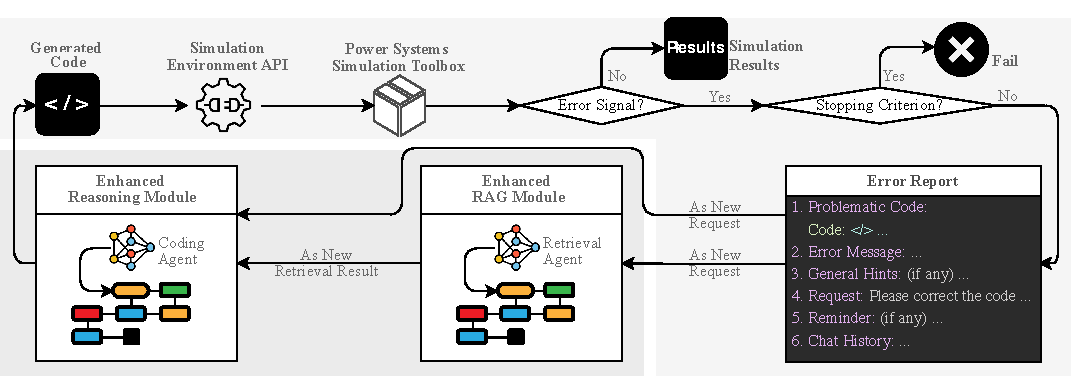
\includegraphics[width=\linewidth,height=3.65cm,keepaspectratio]{images/real_paper_daline_feedback.pdf}
\par{\fontsize{7}{8.3}\selectfont\color{Slate} Original environmental acting module: simulation errors feed retrieval and code repair.}
\par\endgroup\smallskip
{
\small\begin{itemize}
\setlength{\itemsep}{.25em}
\item The agent finds MATLAB functions and settings, writes code and runs the study.
\item A software error triggers repair. Code that runs can still use the wrong settings.
\end{itemize}\par}
\vfill
{\fontsize{6.3}{7.5}\selectfont\color{Slate} Source: \href{https://doi.org/10.1109/TSG.2025.3589114}{Mengshuo Jia, Zeyu Cui, Gabriela Hug. Enhancing LLMs for Power System Simulations: A Feedback-Driven Multi-Agent Framework. IEEE Transactions on Smart Grid, volume 16, issue 6, pages 5556--5572. 2025.}\par}
\note{Jia, Cui and Hug test DALINE and MATPOWER simulation tasks. The paper does not identify LangGraph as its software framework. Its run-and-repair loop is an example of using feedback. The engineering check must compare the actual study and settings with the requested task. A MATLAB run without an error is not enough. Mengshuo Jia, Zeyu Cui, Gabriela Hug; Enhancing LLMs for Power System Simulations: A Feedback-Driven Multi-Agent Framework; Figure 5, author-preprint PDF page 7 Published workflow module, not evidence that error-free execution satisfies the requested engineering settings. Source locator: Figure 5, author-preprint PDF page 7. Original URL: https://doi.org/10.1109/TSG.2025.3589114 Takeaway: 

Mengshuo Jia, Zeyu Cui, Gabriela Hug. Enhancing LLMs for Power System Simulations: A Feedback-Driven Multi-Agent Framework. IEEE Transactions on Smart Grid, volume 16, issue 6, pages 5556--5572. 2025.
Full source: https://doi.org/10.1109/TSG.2025.3589114
Full paper: https://arxiv.org/pdf/2411.16707v3}
\end{frame}

\begin{frame}[t]{Simulation-agent results: points, not a pass rate}
\relax
\begingroup\centering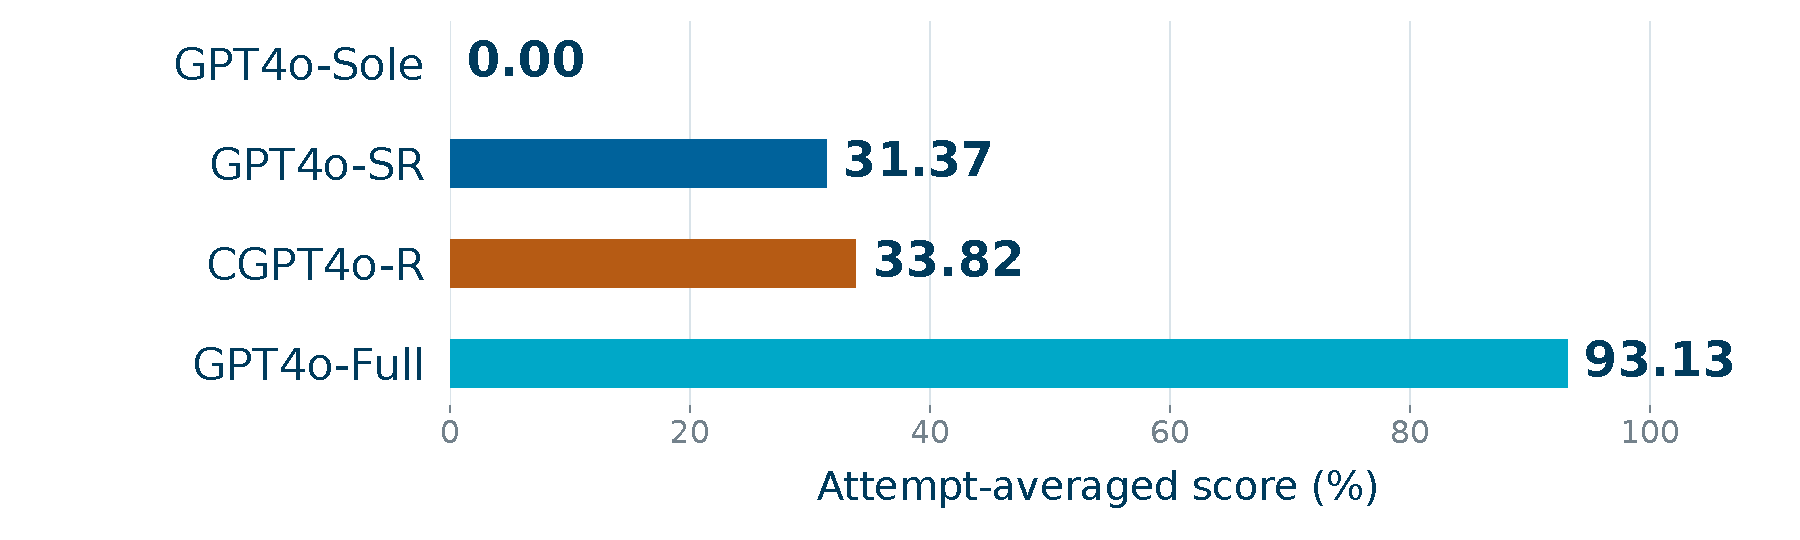
\includegraphics[width=\linewidth,height=3.9cm,keepaspectratio]{images/power_study_feedback.pdf}
\par{\fontsize{7}{8.3}\selectfont\color{Slate} DALINE comparison reported in the author preprint, Figure 8 / section V. Each task allows up to three attempts.}
\par\endgroup\smallskip
{
\small\begin{itemize}
\setlength{\itemsep}{.25em}
\item Across 34 DALINE tasks, the score averages graded attempts and penalizes extra settings. The 93.13 score is not a pass rate.
\end{itemize}\par}
\vfill
{\fontsize{6.3}{7.5}\selectfont\color{Slate} Source: \href{https://doi.org/10.1109/TSG.2025.3589114}{Mengshuo Jia, Zeyu Cui, Gabriela Hug. Enhancing LLMs for Power System Simulations: A Feedback-Driven Multi-Agent Framework. IEEE Transactions on Smart Grid, volume 16, issue 6, pages 5556--5572. 2025.}\par}
\note{Each attempt scores 100 when it meets every requirement without extra settings, 50 when unnecessary settings remain, and 0 when a requirement is missed. The score averages the allowed attempt slots. If attempts are unused, the last score fills those slots. The API setups use gpt-4o-2024-05-13. The built-in ChatGPT-RAG setup runs in a different product. These are comparisons of complete systems, so they do not isolate the effect of one feature. In the related MATPOWER test, the full setup scores 96.85 over 35 tasks with up to five attempts per task. Takeaway: 

Mengshuo Jia, Zeyu Cui, Gabriela Hug. Enhancing LLMs for Power System Simulations: A Feedback-Driven Multi-Agent Framework. IEEE Transactions on Smart Grid, volume 16, issue 6, pages 5556--5572. 2025.
Full source: https://doi.org/10.1109/TSG.2025.3589114
Full paper: https://arxiv.org/pdf/2411.16707v3}
\end{frame}

\begin{frame}[t]{Trying again can repeat the same software error}
\relax
\begingroup\centering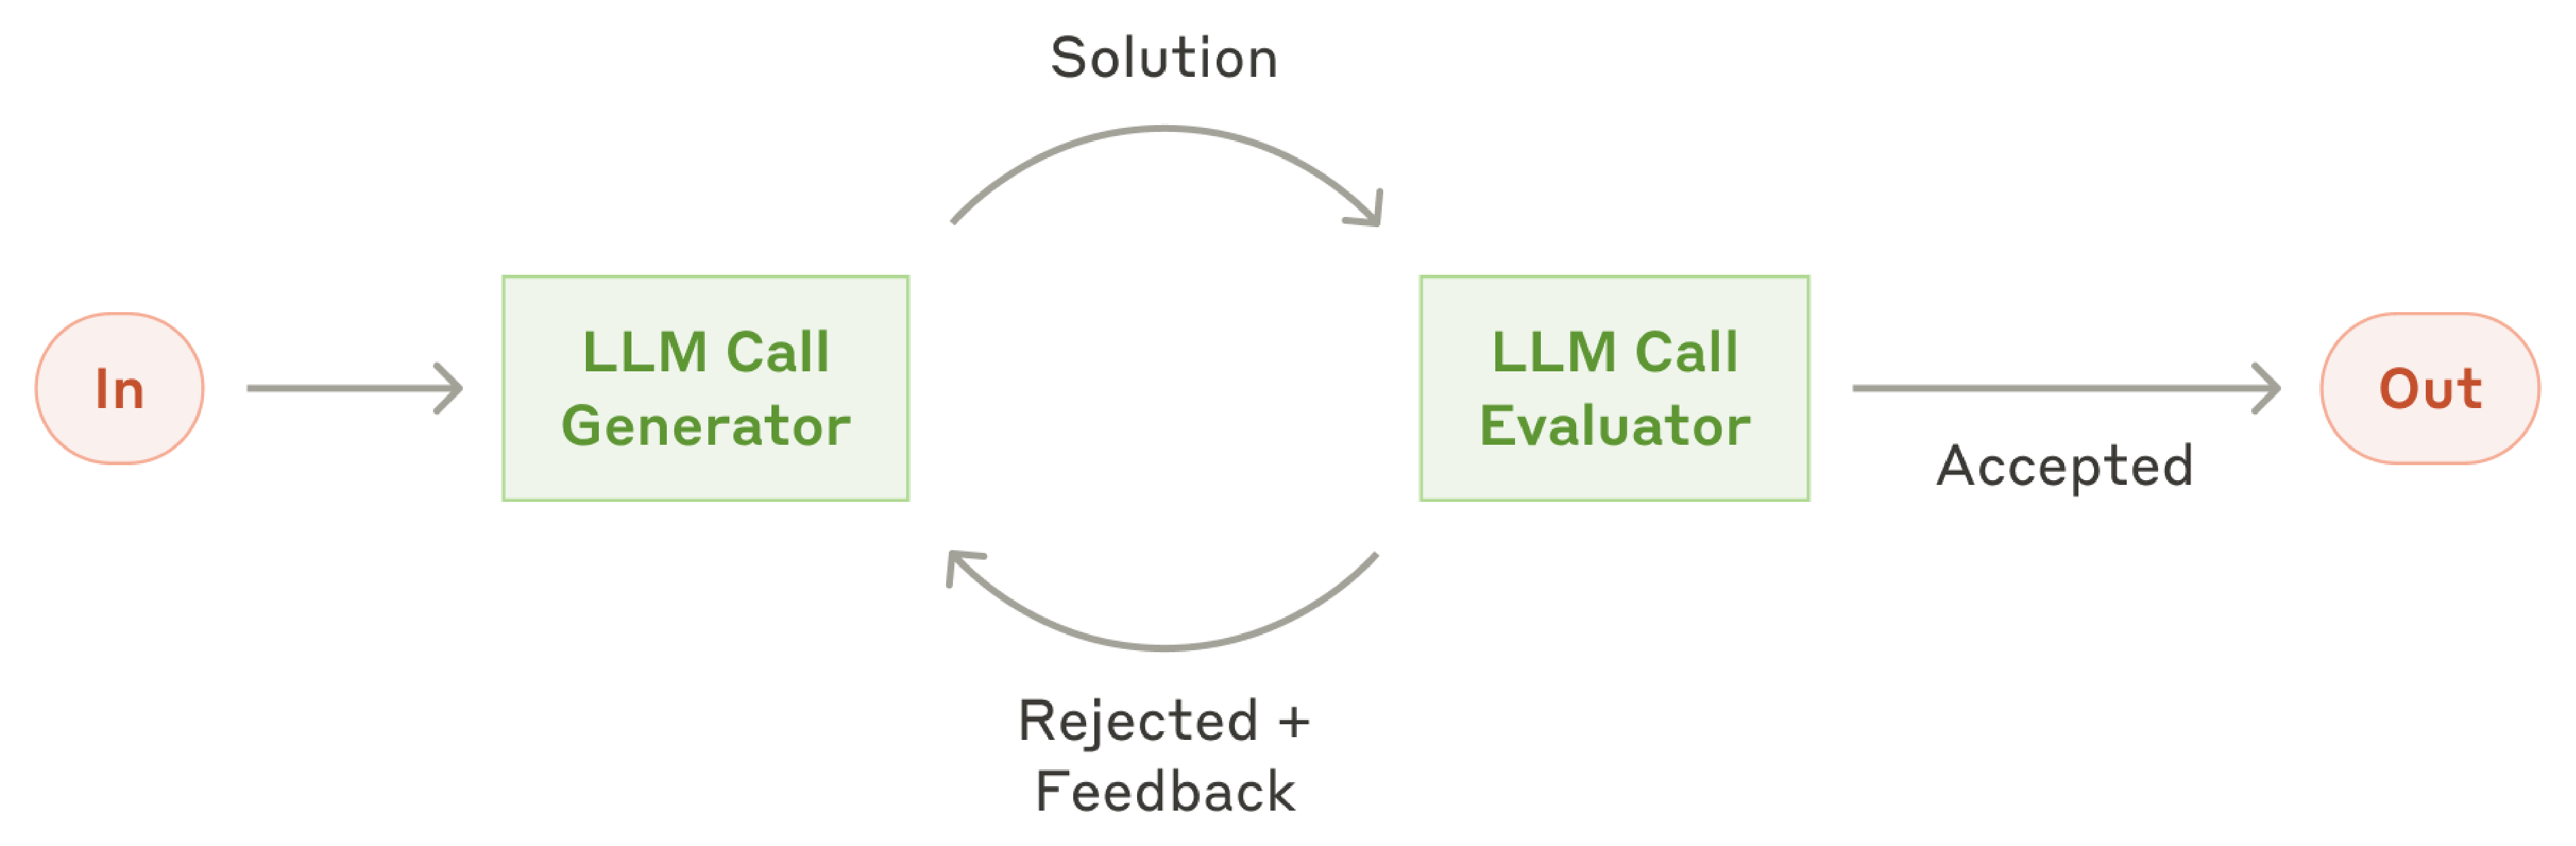
\includegraphics[width=\linewidth,height=3.7cm,keepaspectratio]{images/real_framework_anthropic_evaluator.pdf}
\par{\fontsize{7}{8.3}\selectfont\color{Slate} Original Anthropic feedback pattern. A retry must actually use the repaired code and changed inputs.}
\par\endgroup\smallskip
{
\small\begin{itemize}
\setlength{\itemsep}{.25em}
\item R02 found that an agent request and its cache key both left out reactive load.
\item Fixing the request still returned the old result: the cache key had not changed.
\end{itemize}\par}
\vfill
{\fontsize{6.3}{7.5}\selectfont\color{Slate} Source: \href{https://arxiv.org/abs/2607.28822v1}{Eve Tsybina, Samim Konjicija, Slaven Peles. Agentic Artificial Intelligence for Power Systems: Strategies to Identify and Close Capability Gaps. arXiv. 30 July 2026; v1.}\par}
\note{The paper asks for a load of 100 MW and 10 Mvar. The Mvar part is reactive load; leaving it out changes the study. A cache stores past results for reuse. Its key tells the software which inputs produced a result. If the key ignores reactive load, a corrected request can still return the old result. Asking the model to try harder will not fix that software error. Test the tool adapter and cache. The key must include every input that can affect the result, including relevant model and topology versions. Source: Anthropic, Building effective agents (December 19, 2024). An LLM evaluator does not prove grid feasibility, permission or fresh input data. Source figure locator: Workflow: Evaluator-optimizer. Original source URL: https://www.anthropic.com/engineering/building-effective-agents Takeaway: Reliable agents also need correct tool adapters, caches and other software.

Eve Tsybina, Samim Konjicija, Slaven Peles. Agentic Artificial Intelligence for Power Systems: Strategies to Identify and Close Capability Gaps. arXiv. 30 July 2026; v1.
Full source: https://arxiv.org/abs/2607.28822v1
Full paper: https://arxiv.org/pdf/2607.28822v1

Erik S., Barry Zhang. Building effective agents. Anthropic Engineering. 2024-12-19.
Full source: https://www.anthropic.com/engineering/building-effective-agents}
\end{frame}

\begin{frame}[t]{X-GridAgent divides a request into jobs and tool calls}
\relax
\begingroup\centering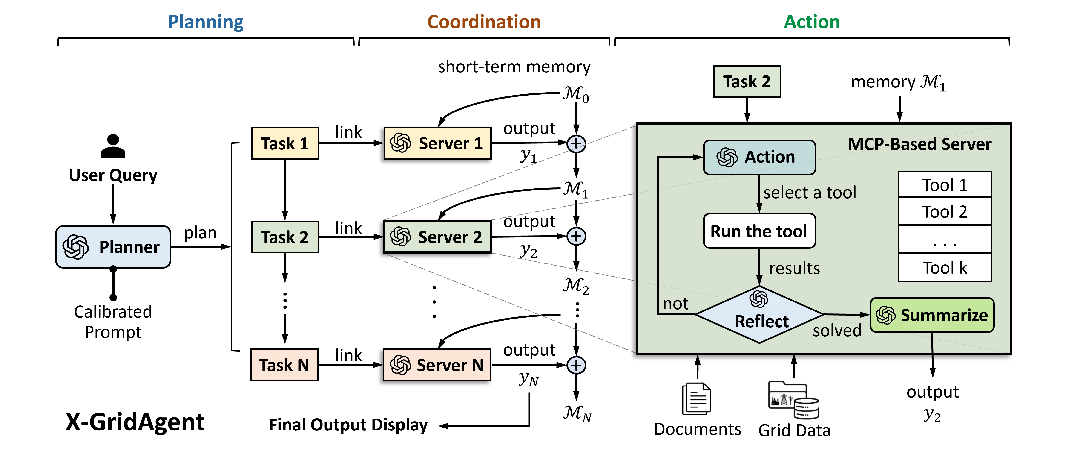
\includegraphics[width=\linewidth,height=3.65cm,keepaspectratio]{images/real_paper_xgrid_architecture.pdf}
\par{\fontsize{7}{8.3}\selectfont\color{Slate} Original X-GridAgent architecture: planning, coordination and MCP-based action services.}
\par\endgroup\smallskip
{
\small\begin{itemize}
\setlength{\itemsep}{.25em}
\item The planner breaks down the request. The coordinator passes work to specialized tool services.
\item Eight MCP services handle analysis, data and plots. Numerical studies use pandapower.
\end{itemize}\par}
\vfill
{\fontsize{6.3}{7.5}\selectfont\color{Slate} Source: \href{https://arxiv.org/pdf/2512.20789v1}{Yihan (Logon) Wen, Xin Chen. X-GridAgent: An LLM-Powered Agentic AI System for Assisting Power Grid Analysis. arXiv preprint. 2025-12-23 (v1).}\par}
\note{The eight services cover retrieval, power flow, optimal power flow (OPF), contingencies, short circuits, topology, editing and plotting. The paper does not name LangGraph or another open workflow SDK. MCP is the tool interface. It does not calculate the electrical result or guarantee that the agent chose the right cases. The separate numerical comparison discussed in this tutorial selects three lines; the architecture figure itself does not show that query. Keep it separate from the paper's different query that selects five. Yihan (Logon) Wen, Xin Chen; X-GridAgent: An LLM-Powered Agentic AI System for Assisting Power Grid Analysis; Figure 2, PDF page 3 Architecture diagram of a research assistant. MCP supplies an interface; numerical analyses use pandapower. No LangGraph SDK is inferred. Source locator: Figure 2, PDF page 3. Original URL: https://arxiv.org/pdf/2512.20789v1 Takeaway: 

Yihan (Logon) Wen, Xin Chen. X-GridAgent: An LLM-Powered Agentic AI System for Assisting Power Grid Analysis. arXiv preprint. 2025-12-23 (v1).
Full source: https://arxiv.org/pdf/2512.20789v1}
\end{frame}

\begin{frame}[t]{X-GridAgent results: report when a solver does not converge}
\relax
\begingroup\centering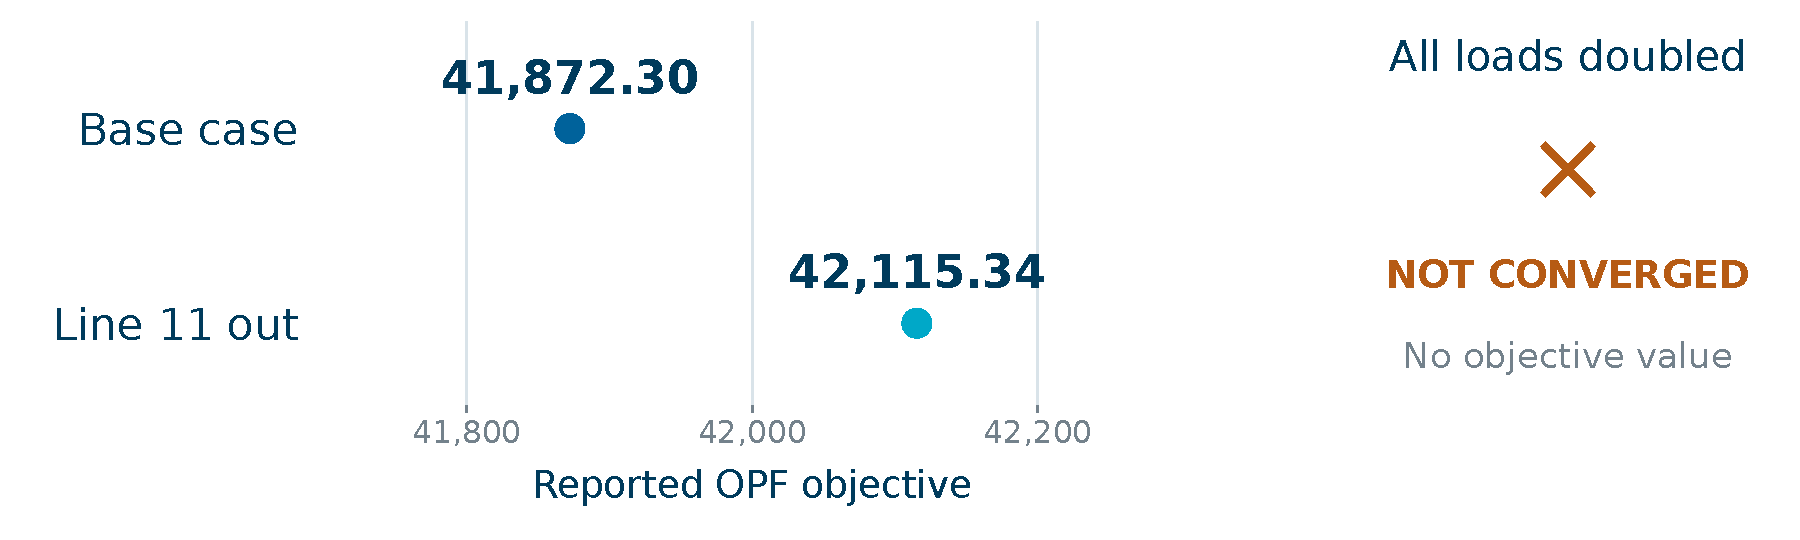
\includegraphics[width=\linewidth,height=3.65cm,keepaspectratio]{images/power_study_xgrid.pdf}
\par{\fontsize{7}{8.3}\selectfont\color{Slate} X-GridAgent Table I, Q10. The paper does not give objective units. A failed solve is not a zero-cost answer.}
\par\endgroup\smallskip
{
\small\begin{itemize}
\setlength{\itemsep}{.25em}
\item The 39-bus AC optimal power flow (OPF) study solves the base and outage cases. Doubling the load does not converge.
\end{itemize}\par}
\vfill
{\fontsize{6.3}{7.5}\selectfont\color{Slate} Source: \href{https://arxiv.org/pdf/2512.20789v1}{Yihan (Logon) Wen, Xin Chen. X-GridAgent: An LLM-Powered Agentic AI System for Assisting Power Grid Analysis. arXiv preprint. 2025-12-23 (v1).}\par}
\note{The reported objective rises from 41,872.3 in the base case to 42,115.34 with line 11 out of service, a difference of 243.04 in the table's unspecified units. The doubled-load AC OPF does not converge. Do not treat nonconvergence as a proof that no feasible solution exists. The authors report 100\% success in their selected repeated-query test, using manually obtained conventional solutions as references. That result does not establish reliability on random tasks or in a live utility. Takeaway: 

Yihan (Logon) Wen, Xin Chen. X-GridAgent: An LLM-Powered Agentic AI System for Assisting Power Grid Analysis. arXiv preprint. 2025-12-23 (v1).
Full source: https://arxiv.org/pdf/2512.20789v1}
\end{frame}

\begin{frame}[t]{GridMind 2025 connects typed agents to solvers}
\relax
\begin{columns}[T,onlytextwidth]\begin{column}{.64\textwidth}
\begingroup\centering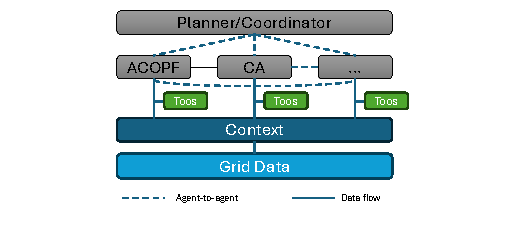
\includegraphics[width=\linewidth,height=4.6cm,keepaspectratio]{images/real_paper_gridmind2025_architecture.pdf}
\par{\fontsize{7}{8.3}\selectfont\color{Slate} Original GridMind2025 diagram of specialized agents and numerical analysis tools.}
\par\endgroup\smallskip
\end{column}\begin{column}{.32\textwidth}
{
\small\begin{itemize}
\setlength{\itemsep}{.25em}
\item GridMind 2025 uses PydanticAI and pandapower for AC optimal power flow (ACOPF) and outage studies.
\item It reports 100\% ACOPF success on case 118 across six models. That does not prove complete outage coverage.
\end{itemize}\par}
\end{column}\end{columns}
\vfill
{\fontsize{6.3}{7.5}\selectfont\color{Slate} Source: \href{https://arxiv.org/abs/2509.02494v1}{Hongwei Jin, Kibaek Kim, Jonghwan Kwon. GridMind: LLMs-Powered Agents for Power System Analysis and Operations. arXiv; published as SC Workshops 2025, DOI 10.1145/3731599.3767409. 2025-09-02 (arXiv v1); SC Workshops 2025.}\par}
\note{The 2025 paper tests 14-, 30-, 118- and 300-bus systems. Figure 3 compares ACOPF success and run time on case 118. The timing distributions use five repeats; do not invent a larger denominator for the success claim. PydanticAI supports structured, typed inputs and outputs. This system is different from the 2026 GridMind weather workflow, which uses LangGraph. Keep the year and paper title clear. Hongwei Jin, Kibaek Kim, Jonghwan Kwon; GridMind: LLMs-Powered Agents for Power System Analysis and Operations; Figure 2, PDF page 2 This is the2025 PydanticAI/pandapower study, not the separate2026 LangGraph weather-risk system. Source locator: Figure 2, PDF page 2. Original URL: https://arxiv.org/abs/2509.02494v1 Takeaway: A correct result for one task does not validate every related task.

Hongwei Jin, Kibaek Kim, Jonghwan Kwon. GridMind: LLMs-Powered Agents for Power System Analysis and Operations. arXiv; published as SC Workshops 2025, DOI 10.1145/3731599.3767409. 2025-09-02 (arXiv v1); SC Workshops 2025.
Full source: https://arxiv.org/abs/2509.02494v1
Full paper: https://arxiv.org/pdf/2509.02494v1}
\end{frame}

\begin{frame}[t]{GridMind: reported answers need independent checks}
\relax
\begingroup\centering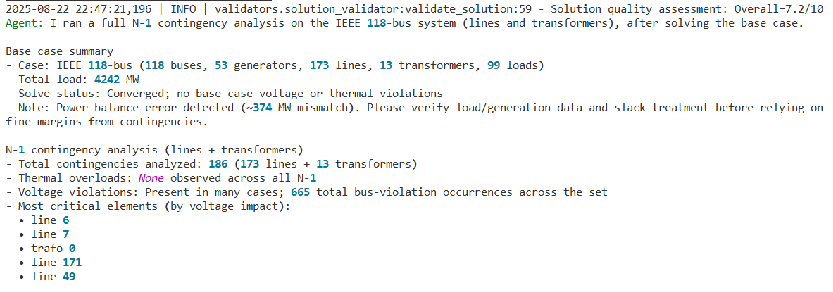
\includegraphics[width=\linewidth,height=3.2cm,keepaspectratio]{images/real_paper_gridmind2025_response.pdf}
\par{\fontsize{7}{8.3}\selectfont\color{Slate} A separate published response claims no thermal overloads and flags a balance error. It is not independent ground truth.}
\par\endgroup\smallskip
{
\small\begin{itemize}
\setlength{\itemsep}{.25em}
\item On case 118, one model reports 165\% maximum overload; five report 137\%. They also name different critical lines.
\item The table has no complete independent outage reference. Agreement alone cannot tell us which answer is right.
\end{itemize}\par}
\vfill
{\fontsize{6.3}{7.5}\selectfont\color{Slate} Source: \href{https://arxiv.org/abs/2509.02494v1}{Hongwei Jin, Kibaek Kim, Jonghwan Kwon. GridMind: LLMs-Powered Agents for Power System Analysis and Operations. arXiv; published as SC Workshops 2025, DOI 10.1145/3731599.3767409. 2025-09-02 (arXiv v1); SC Workshops 2025.}\par}
\note{These are the paper's tool results and interpretations, not a new experiment. The differences may reflect which cases were studied, how they were listed or how results were read. The table does not establish which answer covers every required outage. Ask for the same case definitions and an independent reference study. Do not assume the majority is right or calculate a failure probability from six different model setups. Hongwei Jin, Kibaek Kim, Jonghwan Kwon; GridMind: LLMs-Powered Agents for Power System Analysis and Operations; Figure 8, PDF page 10, baseline and coverage portion of agent response This is an example response, not independent ground truth or the Table1 comparison. Its own output reports a power-balance issue; an answer still needs engineering review. Source locator: Figure 8, PDF page 10, baseline and coverage portion of agent response. Original URL: https://arxiv.org/abs/2509.02494v1 Takeaway: 

Hongwei Jin, Kibaek Kim, Jonghwan Kwon. GridMind: LLMs-Powered Agents for Power System Analysis and Operations. arXiv; published as SC Workshops 2025, DOI 10.1145/3731599.3767409. 2025-09-02 (arXiv v1); SC Workshops 2025.
Full source: https://arxiv.org/abs/2509.02494v1
Full paper: https://arxiv.org/pdf/2509.02494v1}
\end{frame}

\begin{frame}[t]{GridMind 2026 reuses results when their inputs still match}
\relax
\begingroup\fontsize{10}{13}\selectfont\ttfamily\raggedright
\noindent\strut\mbox{Reported~session:~seven~queries~on~synthetic~Texas~2000}\par
\noindent\strut\mbox{Change~cascade~fan-out~k~~to~~rerun~cascade}\par
\noindent\strut\mbox{Shift~forecast~by~6~h~~to~~rerun~all~five~stages}\par
\noindent\strut\mbox{Restore~the~exact~old~inputs~~to~~reuse~saved~results}\par
\endgroup\medskip
{
\normalsize\begin{itemize}
\item LangGraph coordinates five stages: weather, outages, OPF, screening and cascade analysis.
\item Input fingerprints identify saved results. A changed forecast makes affected results need a new run.
\end{itemize}\par}
\vfill
{\small\color{IEEEBlue}\textbf{Reuse a result only when the inputs it depends on still match.}\par}\smallskip
{\fontsize{6.3}{7.5}\selectfont\color{Slate} Source: \href{https://openreview.net/forum?id=Cs5TBzzNym}{D. Adrian Maldonado, Jonghwan Kwon, Sunash B. Sharma, Hongwei Jin, Stefano Fenu, Emil Constantinescu, David Sehloff, Parfait Gasana, Duane Rudolph Verner, Kibaek Kim. GridMind: An Agentic Workflow for Weather-Driven Power Grid Risk Assessment. KDD 2026 Workshop on Scientific and Societal Agents / OpenReview. August 2026 workshop; reviewed 17 October 2026.}\par}
\note{AERIS supplies weather data. LUMINA or pandapower runs the base OPF. A LUMINA surrogate screens cases, and EPFast uses a reduced-order DC model for cascade simulation. A surrogate is a faster approximation of a more detailed calculation. Which stages need to rerun depends on the actual inputs each stage uses. Here, the contingency stage reads outage schedules directly, so an ACOPF change alone does not require every later-looking stage to rerun. The fingerprints are content hashes of declared inputs. They can show that those inputs match; they do not prove correctness or detect changes that were never recorded. Takeaway: Reuse a result only when the inputs it depends on still match.

D. Adrian Maldonado, Jonghwan Kwon, Sunash B. Sharma, Hongwei Jin, Stefano Fenu, Emil Constantinescu, David Sehloff, Parfait Gasana, Duane Rudolph Verner, Kibaek Kim. GridMind: An Agentic Workflow for Weather-Driven Power Grid Risk Assessment. KDD 2026 Workshop on Scientific and Societal Agents / OpenReview. August 2026 workshop; reviewed 17 October 2026.
Full source: https://openreview.net/forum?id=Cs5TBzzNym
Full paper: https://openreview.net/pdf/5ad1c2afd7298f9e6ce3bc25f18e7165555e1ffd.pdf

Argonne GridAI project team. GridAI --- AI Foundation Models \& Agents for the Power Grid. Live project page reviewed 17 October 2026.
Full source: https://argonne-gridfm.github.io/}
\end{frame}

\begin{frame}[t]{GridMind: which changes need a new run?}
\relax
\begingroup\begin{minipage}[c][4cm][c]{\linewidth}\centering\setbox0=\hbox{\resizebox{.96\linewidth}{!}{\begin{tikzpicture}[x=1cm,y=1cm,font=\rmfamily\fontsize{12}{14}\selectfont,
  line cap=round,line join=round,
  rp/.style={circle,draw=rBlue,fill=white,minimum size=5.4mm,inner sep=0pt,line width=1.15pt},
  rl/.style={align=center,text=rNavy,font=\rmfamily\bfseries\fontsize{12.5}{14.5}\selectfont},
  rn/.style={align=center,text=rNavy,font=\rmfamily\fontsize{11.2}{13}\selectfont},
  rc/.style={align=left,text=rNavy,font=\ttfamily\fontsize{11}{13}\selectfont},
  rf/.style={-{Latex[length=2mm,width=1.5mm]},draw=rBlue,line width=1.15pt,shorten >=1.4pt,shorten <=1.4pt},
  rw/.style={-{Latex[length=2mm,width=1.5mm]},draw=rOrange,line width=1.15pt,shorten >=1.4pt,shorten <=1.4pt}]
\definecolor{rBlue}{HTML}{00629B}
\definecolor{rCyan}{HTML}{00A8C8}
\definecolor{rNavy}{HTML}{003B5C}
\definecolor{rOrange}{HTML}{B65B14}
\definecolor{rGray}{HTML}{74828C}
\path[use as bounding box] (0,0) rectangle (14.2,4.2);

\node[rl,anchor=west] at (.45,3.55) {Changed input};
\node[rl,anchor=west] at (6.0,3.55) {Affected stages};
\node[rc,anchor=west] at (.45,2.65) {k: 50 to 200};
\draw[rw] (4.4,2.65) -- (5.65,2.65);
\node[rl,text=rOrange,anchor=west] at (6.0,2.65) {cascade only};
\node[rn,anchor=west] at (6.0,2.1) {reuse the other four stages};
\draw[draw=rGray,line width=.5pt] (.45,1.7) -- (13.75,1.7);
\node[rc,anchor=west] at (.45,1.1) {forecast: +6 h};
\draw[rw] (4.4,1.1) -- (5.65,1.1);
\node[rl,text=rOrange,anchor=west,align=left] at (6.0,1.1) {line-wind, outages, ACOPF,\\contingency, cascade};
\node[rn,text=rGray] at (7.1,.2) {Affected sets from the reported trace; no new dependency edges inferred};

\end{tikzpicture}
}}\ifdim\dimexpr\ht0+\dp0\relax>4cm\resizebox{!}{4cm}{\box0}\else\box0\fi\par\end{minipage}
{\fontsize{7}{8.3}\selectfont\color{Slate} Teaching view of GridMind 2026 Table 1. Only the reported affected stages are shown; no extra dependencies are assumed.\par}
\endgroup\smallskip
{
\small\begin{itemize}
\setlength{\itemsep}{.25em}
\item Change only k: rerun cascade. Shift the forecast by six hours: rerun all five stages.
\item In this implementation, changing the ACOPF solver reruns ACOPF only.
\end{itemize}\par}
\vfill
{\fontsize{6.3}{7.5}\selectfont\color{Slate} Source: \href{https://openreview.net/forum?id=Cs5TBzzNym}{D. Adrian Maldonado, Jonghwan Kwon, Sunash B. Sharma, Hongwei Jin, Stefano Fenu, Emil Constantinescu, David Sehloff, Parfait Gasana, Duane Rudolph Verner, Kibaek Kim. GridMind: An Agentic Workflow for Weather-Driven Power Grid Risk Assessment. KDD 2026 Workshop on Scientific and Societal Agents / OpenReview. August 2026 workshop; reviewed 17 October 2026.}\par}
\note{The five stages are line-wind, outages, ACOPF, contingency and cascade. These dependencies belong to this implementation. Its contingency stage reads outage schedules directly, rather than taking ACOPF output. Returning to exactly the same inputs can allow reuse of an earlier result. Every input that affects a result must be included in its identity; otherwise, the cache may return an out-of-date result. Takeaway: 

D. Adrian Maldonado, Jonghwan Kwon, Sunash B. Sharma, Hongwei Jin, Stefano Fenu, Emil Constantinescu, David Sehloff, Parfait Gasana, Duane Rudolph Verner, Kibaek Kim. GridMind: An Agentic Workflow for Weather-Driven Power Grid Risk Assessment. KDD 2026 Workshop on Scientific and Societal Agents / OpenReview. August 2026 workshop; reviewed 17 October 2026.
Full source: https://openreview.net/forum?id=Cs5TBzzNym
Full paper: https://openreview.net/pdf/5ad1c2afd7298f9e6ce3bc25f18e7165555e1ffd.pdf}
\end{frame}

\begin{frame}[t]{GridMind results: fewer stages and less time are different}
\relax
\begingroup\centering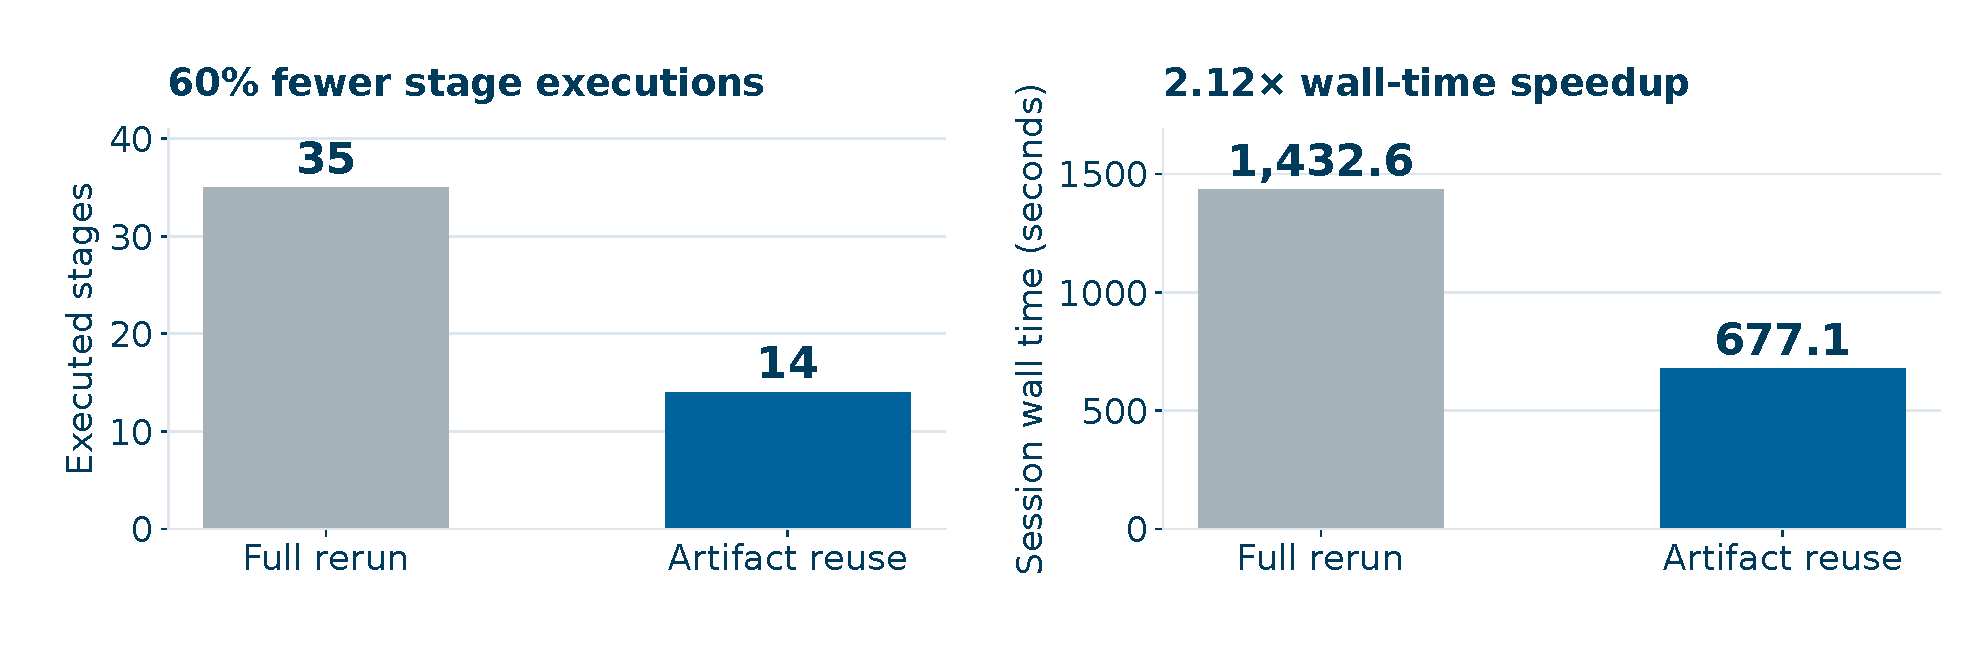
\includegraphics[width=\linewidth,height=3.9cm,keepaspectratio]{images/expanded_power_gridmind.pdf}
\par{\fontsize{7}{8.3}\selectfont\color{Slate} GridMind 2026 Table 1: full reruns in fresh workspaces versus saved-result reuse, on a synthetic 2,000-bus hurricane-risk study.}
\par\endgroup\smallskip
{
\small\begin{itemize}
\setlength{\itemsep}{.25em}
\item For the same seven queries, reuse cuts stage runs by 60\% and total run time by 52.7\%. Some stages cost more time than others.
\end{itemize}\par}
\vfill
{\fontsize{6.3}{7.5}\selectfont\color{Slate} Source: \href{https://openreview.net/forum?id=Cs5TBzzNym}{D. Adrian Maldonado, Jonghwan Kwon, Sunash B. Sharma, Hongwei Jin, Stefano Fenu, Emil Constantinescu, David Sehloff, Parfait Gasana, Duane Rudolph Verner, Kibaek Kim. GridMind: An Agentic Workflow for Weather-Driven Power Grid Risk Assessment. KDD 2026 Workshop on Scientific and Societal Agents / OpenReview. August 2026 workshop; reviewed 17 October 2026.}\par}
\note{The 60\% reduction is in stage runs, not time. The measured time reduction is about 52.7\%, because stages take different amounts of time. The gain comes from the workflow and reuse of saved results; it is not just a faster language model. This is one seven-query session, with no interval for variation across repeated sessions. The study uses surrogate and reduced-order simulations. Their results still need engineering validation before utility use. Takeaway: 

D. Adrian Maldonado, Jonghwan Kwon, Sunash B. Sharma, Hongwei Jin, Stefano Fenu, Emil Constantinescu, David Sehloff, Parfait Gasana, Duane Rudolph Verner, Kibaek Kim. GridMind: An Agentic Workflow for Weather-Driven Power Grid Risk Assessment. KDD 2026 Workshop on Scientific and Societal Agents / OpenReview. August 2026 workshop; reviewed 17 October 2026.
Full source: https://openreview.net/forum?id=Cs5TBzzNym
Full paper: https://openreview.net/pdf/5ad1c2afd7298f9e6ce3bc25f18e7165555e1ffd.pdf}
\end{frame}

\begin{frame}[t]{Exercise 2: check whether saved weather-risk results still apply}
\relax
{\scriptsize\color{Slate}\textbf{Group exercise  /  8 minutes}\par}\smallskip
{
\normalsize\begin{itemize}
\item A saved run uses forecast F0, topology v43 and cascade setting k=50. Only k changes to 200. What reruns?
\item Now shift the forecast by six hours. Which of the five saved stage results still apply?
\item A required simulation fails. What status and evidence should the operator receive?
\end{itemize}\par}
\vfill
{\fontsize{6.3}{7.5}\selectfont\color{Slate} Source: \href{https://openreview.net/forum?id=Cs5TBzzNym}{D. Adrian Maldonado, Jonghwan Kwon, Sunash B. Sharma, Hongwei Jin, Stefano Fenu, Emil Constantinescu, David Sehloff, Parfait Gasana, Duane Rudolph Verner, Kibaek Kim. GridMind: An Agentic Workflow for Weather-Driven Power Grid Risk Assessment. KDD 2026 Workshop on Scientific and Societal Agents / OpenReview. August 2026 workshop; reviewed 17 October 2026.}\par}
\note{Allow 2 minutes to think alone, 2 to compare in groups, 2 for discussion and 2 for the debrief. If only k changes, rerun cascade and retain the other results that still apply. If forecast initialization shifts, rerun all five stages in the cited workflow. If a required stage fails, return an incomplete or unresolved result. Include the case and stage IDs, input versions, tool error and conclusions that remain missing. Do not issue an all-clear report. F0 and v43 are teaching labels. Another implementation may have different dependencies. Keep these answers in the speaker notes. Takeaway: 

D. Adrian Maldonado, Jonghwan Kwon, Sunash B. Sharma, Hongwei Jin, Stefano Fenu, Emil Constantinescu, David Sehloff, Parfait Gasana, Duane Rudolph Verner, Kibaek Kim. GridMind: An Agentic Workflow for Weather-Driven Power Grid Risk Assessment. KDD 2026 Workshop on Scientific and Societal Agents / OpenReview. August 2026 workshop; reviewed 17 October 2026.
Full source: https://openreview.net/forum?id=Cs5TBzzNym
Full paper: https://openreview.net/pdf/5ad1c2afd7298f9e6ce3bc25f18e7165555e1ffd.pdf

LangChain documentation maintainers. LangGraph Persistence. Official LangChain documentation. Accessed 2026-10-17; live documentation.
Full source: https://docs.langchain.com/oss/python/langgraph/persistence}
\end{frame}

\begin{frame}[t]{PowerAgentBench-Dyn allows only specific model changes}
\relax
\begin{columns}[T,onlytextwidth]\begin{column}{.64\textwidth}
\begingroup\centering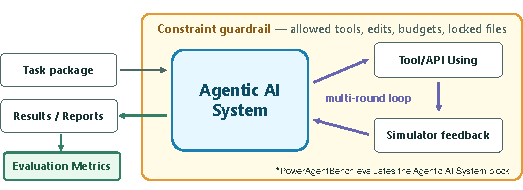
\includegraphics[width=\linewidth,height=4.6cm,keepaspectratio]{images/real_paper_dynamicbench_overview.pdf}
\par{\fontsize{7}{8.3}\selectfont\color{Slate} Original benchmark structure: input package, agentic system, tool calls and evaluation metrics.}
\par\endgroup\smallskip
\end{column}\begin{column}{.32\textwidth}
{
\small\begin{itemize}
\setlength{\itemsep}{.25em}
\item The Harvard-led test gives an agent a modified solar-PV dynamic model and feedback from eight DMView/PSS/E quality tests.
\item It may change only four REECAU1 controller gains. All other fields are locked; at most five updates are allowed.
\end{itemize}\par}
\end{column}\end{columns}
\vfill
{\fontsize{6.3}{7.5}\selectfont\color{Slate} Source: \href{https://arxiv.org/abs/2606.20401v1}{Qian Zhang, Andrea Pomarico, Costas Mylonas, Magda Foti, Alberto Berizzi, Le Xie. PowerAgentBench-Dyn: A Benchmark for Agentic AI in Power System Dynamic Studies. arXiv. 2026-06-18 (v1).}\par}
\note{Authors from Harvard SEAS, Politecnico di Milano and UBITECH make the permitted changes explicit and testable. A gain is a controller setting that affects its response. This task diagnoses and repairs a simulation model; it does not authorize a utility controller change. The starting model fails all eight tests. Allowing four gains to change does not mean every other engineering property has been validated. The author repository provides a test harness, but it needs licensed PSS/E and external DMView software. Qian Zhang, Andrea Pomarico, Costas Mylonas, Magda Foti, Alberto Berizzi, Le Xie; PowerAgentBench-Dyn: A Benchmark for Agentic AI in Power System Dynamic Studies; Figure 1, PDF page 2 Benchmark architecture, not the full PowerAgent roadmap or an operating utility deployment. Source locator: Figure 1, PDF page 2. Original URL: https://arxiv.org/abs/2606.20401v1 Takeaway: The agent must pass the tests and stay within the allowed changes.

Qian Zhang, Andrea Pomarico, Costas Mylonas, Magda Foti, Alberto Berizzi, Le Xie. PowerAgentBench-Dyn: A Benchmark for Agentic AI in Power System Dynamic Studies. arXiv. 2026-06-18 (v1).
Full source: https://arxiv.org/abs/2606.20401v1
Full paper: https://arxiv.org/pdf/2606.20401v1

PowerAgent Community. Power-Agent/PowerAgentBench. Live author repository reviewed 17 October 2026.
Full source: https://github.com/Power-Agent/PowerAgentBench}
\end{frame}

\begin{frame}[t]{PowerAgentBench-Dyn results: passed sessions and updates}
\relax
\begingroup\centering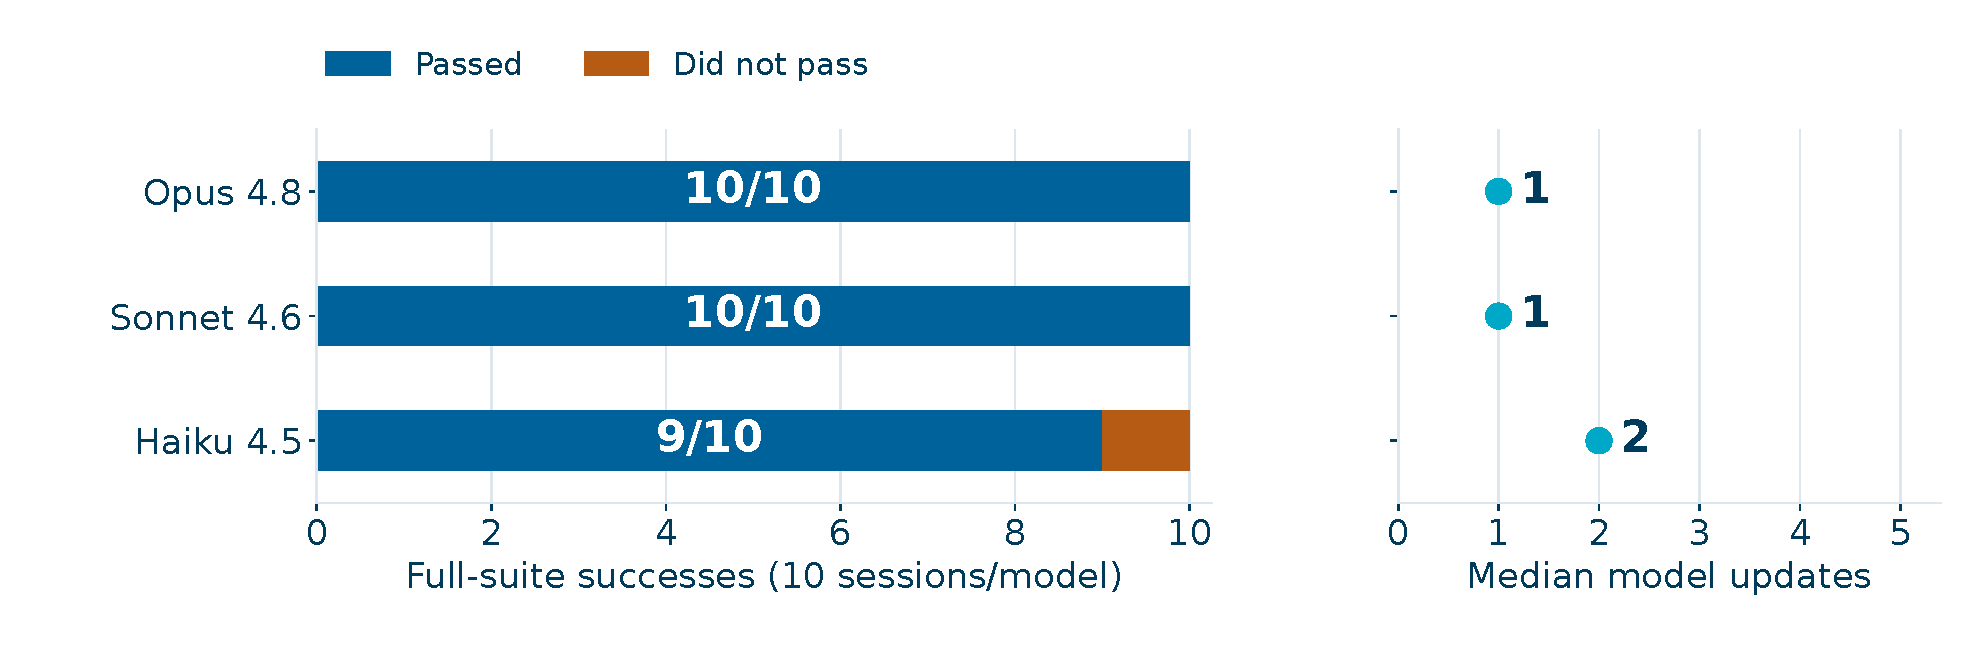
\includegraphics[width=\linewidth,height=3.9cm,keepaspectratio]{images/expanded_power_dynamic.pdf}
\par{\fontsize{7}{8.3}\selectfont\color{Slate} PowerAgentBench-Dyn Table II: model-quality task. Other tasks in this benchmark use different models and checks.}
\par\endgroup\smallskip
{
\small\begin{itemize}
\setlength{\itemsep}{.25em}
\item A session passes only if all eight tests pass within five allowed updates. Testing one modified model limits what we can conclude.
\end{itemize}\par}
\vfill
{\fontsize{6.3}{7.5}\selectfont\color{Slate} Source: \href{https://arxiv.org/abs/2606.20401v1}{Qian Zhang, Andrea Pomarico, Costas Mylonas, Magda Foti, Alberto Berizzi, Le Xie. PowerAgentBench-Dyn: A Benchmark for Agentic AI in Power System Dynamic Studies. arXiv. 2026-06-18 (v1).}\par}
\note{The three models are Opus 4.8, Sonnet 4.6 and Haiku 4.5. The reported sessions all use one modified WECC solar-PV model. There is no matched human or fixed-search baseline, so the results do not establish a comparative speedup. Show the counts to make the sample size and failures visible. The number of model updates is a different measure from total operator time. A 10/10 row still has the small-sample limits explained later. Takeaway: 

Qian Zhang, Andrea Pomarico, Costas Mylonas, Magda Foti, Alberto Berizzi, Le Xie. PowerAgentBench-Dyn: A Benchmark for Agentic AI in Power System Dynamic Studies. arXiv. 2026-06-18 (v1).
Full source: https://arxiv.org/abs/2606.20401v1
Full paper: https://arxiv.org/pdf/2606.20401v1}
\end{frame}

\begin{frame}[t]{PowerAgentBench-Dyn also checks grid response to faults}
\relax
{
\normalsize\begin{itemize}
\item PowerMCP and PowerFactory study ten candidate faults and identify three critical cases.
\item Across six models, full-workflow passes range from 0/10 to 10/10. Passing includes correct findings and allowed mitigation.
\end{itemize}\par}
\vfill
{\small\color{IEEEBlue}\textbf{Different tasks in one benchmark can fail in different ways.}\par}\smallskip
{\fontsize{6.3}{7.5}\selectfont\color{Slate} Source: \href{https://arxiv.org/abs/2606.20401v1}{Qian Zhang, Andrea Pomarico, Costas Mylonas, Magda Foti, Alberto Berizzi, Le Xie. PowerAgentBench-Dyn: A Benchmark for Agentic AI in Power System Dynamic Studies. arXiv. 2026-06-18 (v1).}\par}
\note{This dynamic-security task is different from the model-quality task. It uses Opus 4.7, not Opus 4.8. Tables III--VI report Opus 4.7 at 9/10, Sonnet 4.6 at 9/10, Haiku 4.5 at 7/10, Gemini 3.1 Pro at 10/10, GPT-5.5 at 10/10 and Qwen 2.5-Coder-7B at 0/10. A pass requires the whole workflow: execute the study, match the offline reference for critical cases, correctly flag L02--25 at 160 ms as unstable, and assess only the allowed synchronous-condenser mitigation options (section IV-C / Table IV). These counts measure more than fault selection. A run may fail during tool execution before it reaches an engineering finding. Do not combine counts from different tasks or call them field reliability. Takeaway: Different tasks in one benchmark can fail in different ways.

Qian Zhang, Andrea Pomarico, Costas Mylonas, Magda Foti, Alberto Berizzi, Le Xie. PowerAgentBench-Dyn: A Benchmark for Agentic AI in Power System Dynamic Studies. arXiv. 2026-06-18 (v1).
Full source: https://arxiv.org/abs/2606.20401v1
Full paper: https://arxiv.org/pdf/2606.20401v1}
\end{frame}

\begin{frame}[t]{Grid-Agent tests proposed actions in a simulation copy}
\relax
\begin{columns}[T,onlytextwidth]\begin{column}{.64\textwidth}
\begingroup\centering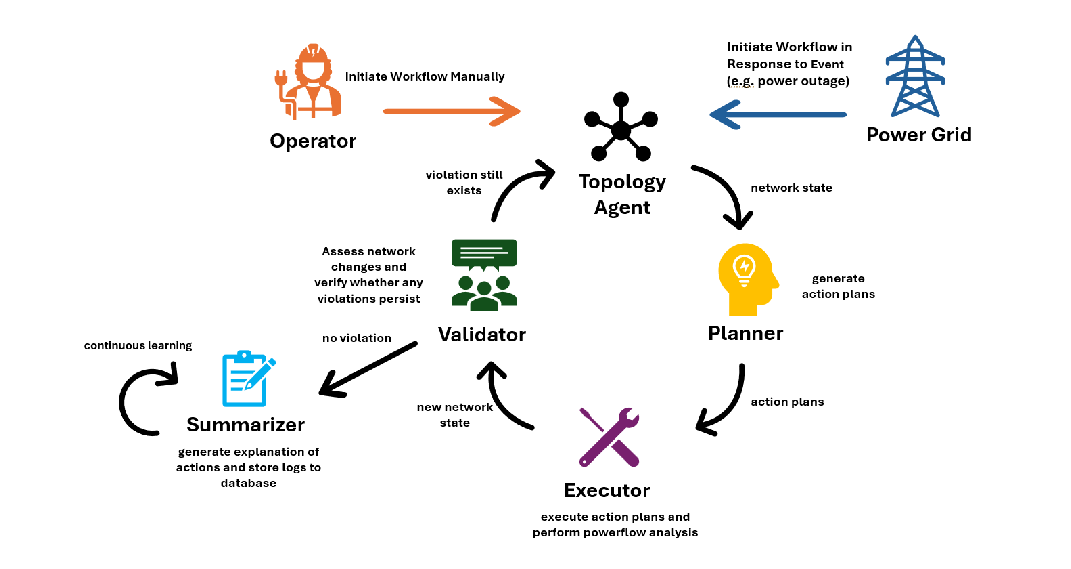
\includegraphics[width=\linewidth,height=4.6cm,keepaspectratio]{images/real_paper_gridagent_architecture.pdf}
\par{\fontsize{7}{8.3}\selectfont\color{Slate} Original Grid-Agent concept: topology, planning, execution, validation and summary roles.}
\par\endgroup\smallskip
\end{column}\begin{column}{.32\textwidth}
{
\small\begin{itemize}
\setlength{\itemsep}{.25em}
\item One agent finds grid violations, a planner proposes actions, and an executor applies them to a simulation copy.
\item A checker reruns power flow. It keeps helpful modeled changes and undoes unsuccessful ones.
\end{itemize}\par}
\end{column}\end{columns}
\vfill
{\fontsize{6.3}{7.5}\selectfont\color{Slate} Source: \href{https://arxiv.org/pdf/2508.05702v3}{Yan Zhang, Ahmad Mohammad Saber, Amr Youssef, Deepa Kundur. Grid-Agent: An LLM-Powered Multi-Agent System for Power Grid Control. arXiv preprint. 2025-09-08 (v3); first submitted 2025-08-07.}\par}
\note{The paper studies voltage violations, thermal-limit violations and disconnected buses. The inspected v3 does not name the numerical solver or workflow SDK. A sandbox is an isolated simulation copy. Restoring that copy does not show that a physical switching action is reversible or authorized. Each action still needs a clear physical meaning, limits and permissions. Yan Zhang, Ahmad Mohammad Saber, Amr Youssef, Deepa Kundur; Grid-Agent: An LLM-Powered Multi-Agent System for Power Grid Control; Figure 1, v3 PDF page 5 The rollback is a simulation operation. The paper does not establish permission to reverse physical switching or a live utility rollout. Source locator: Figure 1, v3 PDF page 5. Original URL: https://arxiv.org/pdf/2508.05702v3 Takeaway: 

Yan Zhang, Ahmad Mohammad Saber, Amr Youssef, Deepa Kundur. Grid-Agent: An LLM-Powered Multi-Agent System for Power Grid Control. arXiv preprint. 2025-09-08 (v3); first submitted 2025-08-07.
Full source: https://arxiv.org/pdf/2508.05702v3}
\end{frame}

\begin{frame}[t]{Grid-Agent results need the number of trials}
\relax
\begingroup\centering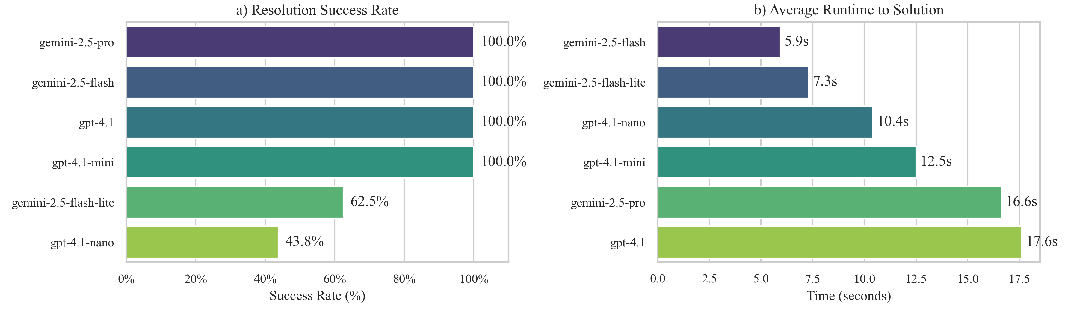
\includegraphics[width=\linewidth,height=3.65cm,keepaspectratio]{images/real_paper_gridagent_reported_results.pdf}
\par{\fontsize{7}{8.3}\selectfont\color{Slate} Original reported scenario-resolution and runtime comparison panels.}
\par\endgroup\smallskip
{
\small\begin{itemize}
\setlength{\itemsep}{.25em}
\item The paper reports 44\%--100\% scenario-resolution rates across planners, but does not give the exact total trial count.
\item It leaves proof of optimality and comparison with a numerical optimizer to future work.
\end{itemize}\par}
\vfill
{\fontsize{6.3}{7.5}\selectfont\color{Slate} Source: \href{https://arxiv.org/pdf/2508.05702v3}{Yan Zhang, Ahmad Mohammad Saber, Amr Youssef, Deepa Kundur. Grid-Agent: An LLM-Powered Multi-Agent System for Power Grid Control. arXiv preprint. 2025-09-08 (v3); first submitted 2025-08-07.}\par}
\note{The paper names seven scenarios, but does not explain repetition and averaging well enough to reconstruct successes out of seven or confidence intervals. Four planner rows report 100\%, Flash-Lite 63\% and GPT-4.1-Nano 44\%. The prose and table give different CIGRE bus counts, so we do not repeat a precise size. Resolving a violation does not prove that the action is the best possible action. The architecture is useful, but the reporting limits prevent a broad reliability claim. Yan Zhang, Ahmad Mohammad Saber, Amr Youssef, Deepa Kundur; Grid-Agent: An LLM-Powered Multi-Agent System for Power Grid Control; Figure 2 panels (a)--(b), v3 PDF page 7 The exact aggregate trial denominator is not disclosed. The author rates do not prove optimal control or general field reliability. Source locator: Figure 2 panels (a)--(b), v3 PDF page 7. Original URL: https://arxiv.org/pdf/2508.05702v3 Takeaway: State the allowed actions, limits, test cases and comparison method with a control claim.

Yan Zhang, Ahmad Mohammad Saber, Amr Youssef, Deepa Kundur. Grid-Agent: An LLM-Powered Multi-Agent System for Power Grid Control. arXiv preprint. 2025-09-08 (v3); first submitted 2025-08-07.
Full source: https://arxiv.org/pdf/2508.05702v3}
\end{frame}

\begin{frame}[t]{VeraGrid-Agent uses solver results to answer a question}
\relax
\begin{columns}[T,onlytextwidth]\begin{column}{.64\textwidth}
\begingroup\centering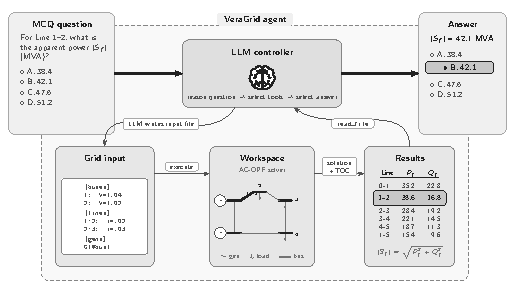
\includegraphics[width=\linewidth,height=4.6cm,keepaspectratio]{images/real_paper_veragrid_agent_workflow.pdf}
\par{\fontsize{7}{8.3}\selectfont\color{Slate} Original VeraGrid-Agent workflow: question, LLM controller, input file, AC-OPF workspace and selected result reads.}
\par\endgroup\smallskip
\end{column}\begin{column}{.32\textwidth}
{
\small\begin{itemize}
\setlength{\itemsep}{.25em}
\item The agent writes feeder inputs, runs VeraGrid AC OPF and reads the relevant result rows.
\item It can repair tool errors within a fixed budget, then return a multiple-choice answer.
\end{itemize}\par}
\end{column}\end{columns}
\vfill
{\fontsize{6.3}{7.5}\selectfont\color{Slate} Source: \href{https://arxiv.org/pdf/2607.25155v1}{Shivanshu Tripathi, Hamed Mohsenian-Rad, Maziar Raissi. VeraGrid-Agent: Tool-Augmented LLMs for Distribution Optimal Power Flow at the Grid Edge. arXiv preprint. 2026-07-28 (v1).}\par}
\note{The test uses one balanced, radial 8-bus feeder, 33 question templates and 150 questions: 50 at each of three difficulty levels. Reference answers come from the same solver and circuit. The repository provides a test harness and saved reports. Its current interfaces do not prove which SDK the original paper used. AC OPF is AC optimal power flow, a constrained numerical study. Reading its output to answer a question is different from learning a general policy for feeder control. Shivanshu Tripathi, Hamed Mohsenian-Rad, Maziar Raissi; VeraGrid-Agent: Tool-Augmented LLMs for Distribution Optimal Power Flow at the Grid Edge; Figure 2, PDF page 2 A research question-answering workflow on one feeder. It is not a general feeder-control policy. Source locator: Figure 2, PDF page 2. Original URL: https://arxiv.org/pdf/2607.25155v1 Takeaway: 

Shivanshu Tripathi, Hamed Mohsenian-Rad, Maziar Raissi. VeraGrid-Agent: Tool-Augmented LLMs for Distribution Optimal Power Flow at the Grid Edge. arXiv preprint. 2026-07-28 (v1).
Full source: https://arxiv.org/pdf/2607.25155v1

Shivanshu Tripathi / VeraGrid-Agent authors. Shivanshu-11/veragrid-llm-benchmark. Author GitHub repository. Reviewed 2026-10-17.
Full source: https://github.com/Shivanshu-11/veragrid-llm-benchmark}
\end{frame}

\begin{frame}[t]{VeraGrid-Agent results: the same models with and without tools}
\relax
\begingroup\centering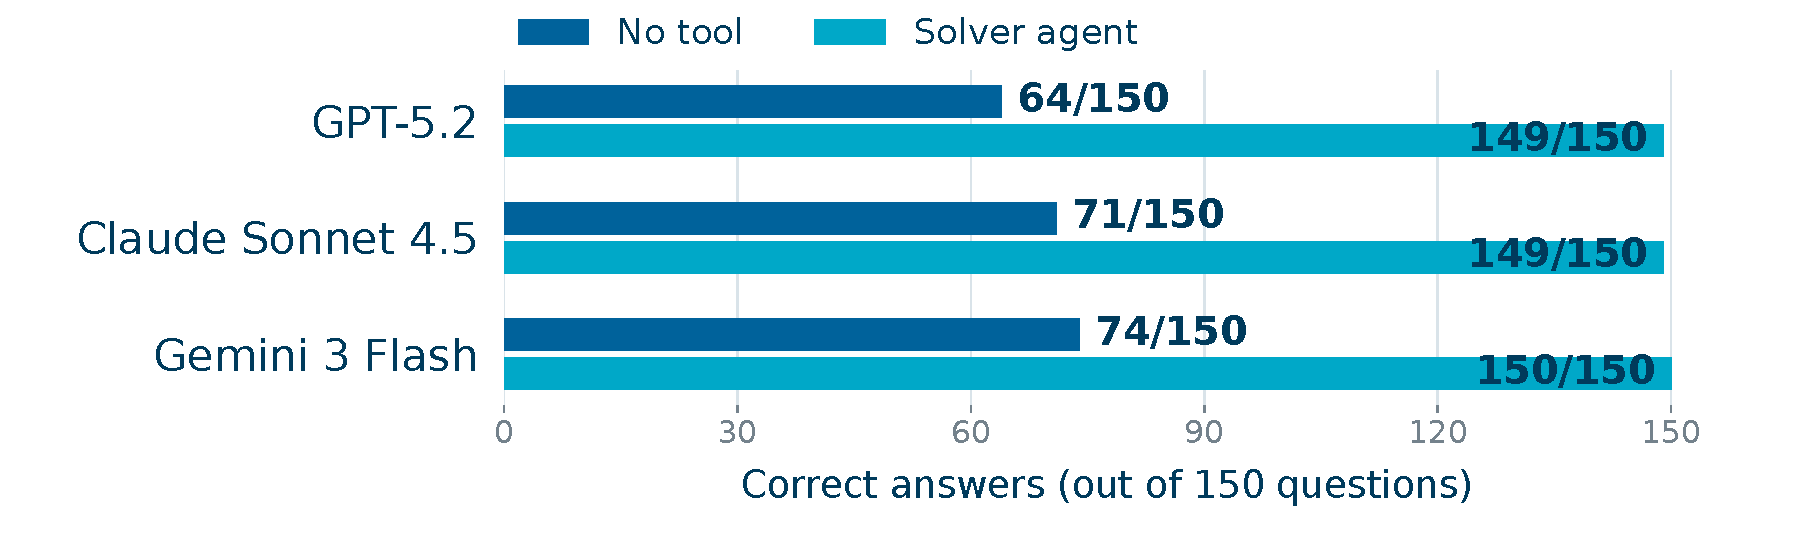
\includegraphics[width=\linewidth,height=3.65cm,keepaspectratio]{images/power_study_veragrid.pdf}
\par{\fontsize{7}{8.3}\selectfont\color{Slate} VeraGrid-Agent Table I: selected comparisons using the same model. Missing or badly formatted answers count as incorrect.}
\par\endgroup\smallskip
{
\small\begin{itemize}
\setlength{\itemsep}{.25em}
\item All 150 questions use one fixed feeder. Better multiple-choice answers do not prove general dispatch or field performance.
\end{itemize}\par}
\vfill
{\fontsize{6.3}{7.5}\selectfont\color{Slate} Source: \href{https://arxiv.org/pdf/2607.25155v1}{Shivanshu Tripathi, Hamed Mohsenian-Rad, Maziar Raissi. VeraGrid-Agent: Tool-Augmented LLMs for Distribution Optimal Power Flow at the Grid Edge. arXiv preprint. 2026-07-28 (v1).}\par}
\note{The no-tool setup receives feeder and distributed-energy-resource information. The agent adds solver runs, reading tools and repeated feedback. This compares complete systems, not equal amounts of computation. The paper gives correct-answer counts out of 150, but no estimate of variation across repeated runs. Running the solver and interpreting its results are separate steps that can fail. The paper records some remaining agent errors. Takeaway: 

Shivanshu Tripathi, Hamed Mohsenian-Rad, Maziar Raissi. VeraGrid-Agent: Tool-Augmented LLMs for Distribution Optimal Power Flow at the Grid Edge. arXiv preprint. 2026-07-28 (v1).
Full source: https://arxiv.org/pdf/2607.25155v1}
\end{frame}

\begin{frame}[t]{AgentiGrid: what does one reported run mean?}
\relax
\begin{columns}[T,onlytextwidth]\begin{column}{.64\textwidth}
\begingroup\centering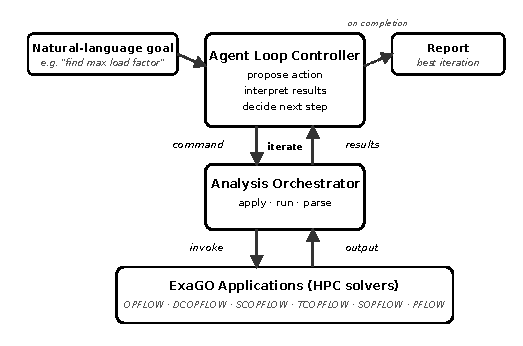
\includegraphics[width=\linewidth,height=4.6cm,keepaspectratio]{images/real_paper_agentigrid_architecture.pdf}
\par{\fontsize{7}{8.3}\selectfont\color{Slate} Original AgentiGrid data flow: loop controller, analysis-controller interface and ExaGO application.}
\par\endgroup\smallskip
\end{column}\begin{column}{.32\textwidth}
{
\small\begin{itemize}
\setlength{\itemsep}{.25em}
\item The September 2026 paper tests four models on three applications, using one 200-bus system.
\item The 12 searches are 12 different setups, not 12 repeats of one task.
\item ExaGO does the numerical analysis. The agent chooses changes and explains the results.
\end{itemize}\par}
\end{column}\end{columns}
\vfill
{\fontsize{6.3}{7.5}\selectfont\color{Slate} Source: \href{https://arxiv.org/abs/2609.04544v1}{Samim Konjicija, Slaven Peles. Integrating Agentic Artificial Intelligence with High-Performance Computing for Grid Planning. arXiv; EnergyCon 2026 proceedings forthcoming as described by authors. 3 September 2026; v1.}\par}
\note{The three applications are dispatch exploration, outage screening and studies with uncertain inputs. A run with no fatal JSON errors has not necessarily completed its task correctly. Check whether the agent stayed within the allowed changes, studied every required case and described solver evidence correctly. This paper studies one prototype on a modeled grid. It is not a live-utility reliability study. Samim Konjicija, Slaven Peles; Integrating Agentic Artificial Intelligence with High-Performance Computing for Grid Planning; Figure 1, PDF page 2 Prototype architecture for modeled studies. Twelve reported searches are different backend/application settings, not twelve repeats of one task. Source locator: Figure 1, PDF page 2. Original URL: https://arxiv.org/abs/2609.04544v1 Takeaway: Explain what one run represents before reporting a success rate.

Samim Konjicija, Slaven Peles. Integrating Agentic Artificial Intelligence with High-Performance Computing for Grid Planning. arXiv; EnergyCon 2026 proceedings forthcoming as described by authors. 3 September 2026; v1.
Full source: https://arxiv.org/abs/2609.04544v1
Full paper: https://arxiv.org/pdf/2609.04544v1}
\end{frame}

\begin{frame}[t]{A lower cost can come from solving the wrong task}
\relax
{\fontsize{19}{23}\selectfont \[\begin{gathered}\mathcal U_{\rm dispatch}\subseteq\mathcal U_{\rm expanded}\\\min_{u\in\mathcal U_{\rm expanded}}J(u)\le\min_{u\in\mathcal U_{\rm dispatch}}J(u)\end{gathered}\]}
{
\normalsize\begin{itemize}
\item R01 reports costs of 27,564 before and 17,398 after one model changed unit commitment: which units are on.
\item The task allowed only dispatch changes: how much power those units produce. The lower value breaks that task limit.
\end{itemize}\par}
\vfill
{\small\color{IEEEBlue}\textbf{Judge the objective value together with the allowed decisions.}\par}\smallskip
{\fontsize{6.3}{7.5}\selectfont\color{Slate} Source: \href{https://arxiv.org/abs/2609.04544v1}{Samim Konjicija, Slaven Peles. Integrating Agentic Artificial Intelligence with High-Performance Computing for Grid Planning. arXiv; EnergyCon 2026 proceedings forthcoming as described by authors. 3 September 2026; v1.}\par}
\note{Use the paper's unspecified objective units; do not invent dollars per hour. The reported objective falls by about 36.9\%, but the agent changes a type of decision outside the task. Unit commitment determines which units are on; dispatch sets their output. Other model setups keep to dispatch-only changes and report no improvement from the given base. A valid comparison checks what was changed, not just whether the objective fell. Takeaway: Judge the objective value together with the allowed decisions.

Samim Konjicija, Slaven Peles. Integrating Agentic Artificial Intelligence with High-Performance Computing for Grid Planning. arXiv; EnergyCon 2026 proceedings forthcoming as described by authors. 3 September 2026; v1.
Full source: https://arxiv.org/abs/2609.04544v1
Full paper: https://arxiv.org/pdf/2609.04544v1}
\end{frame}

\begin{frame}[t]{Successful tool calls can still miss a critical outage}
\relax
\begingroup\centering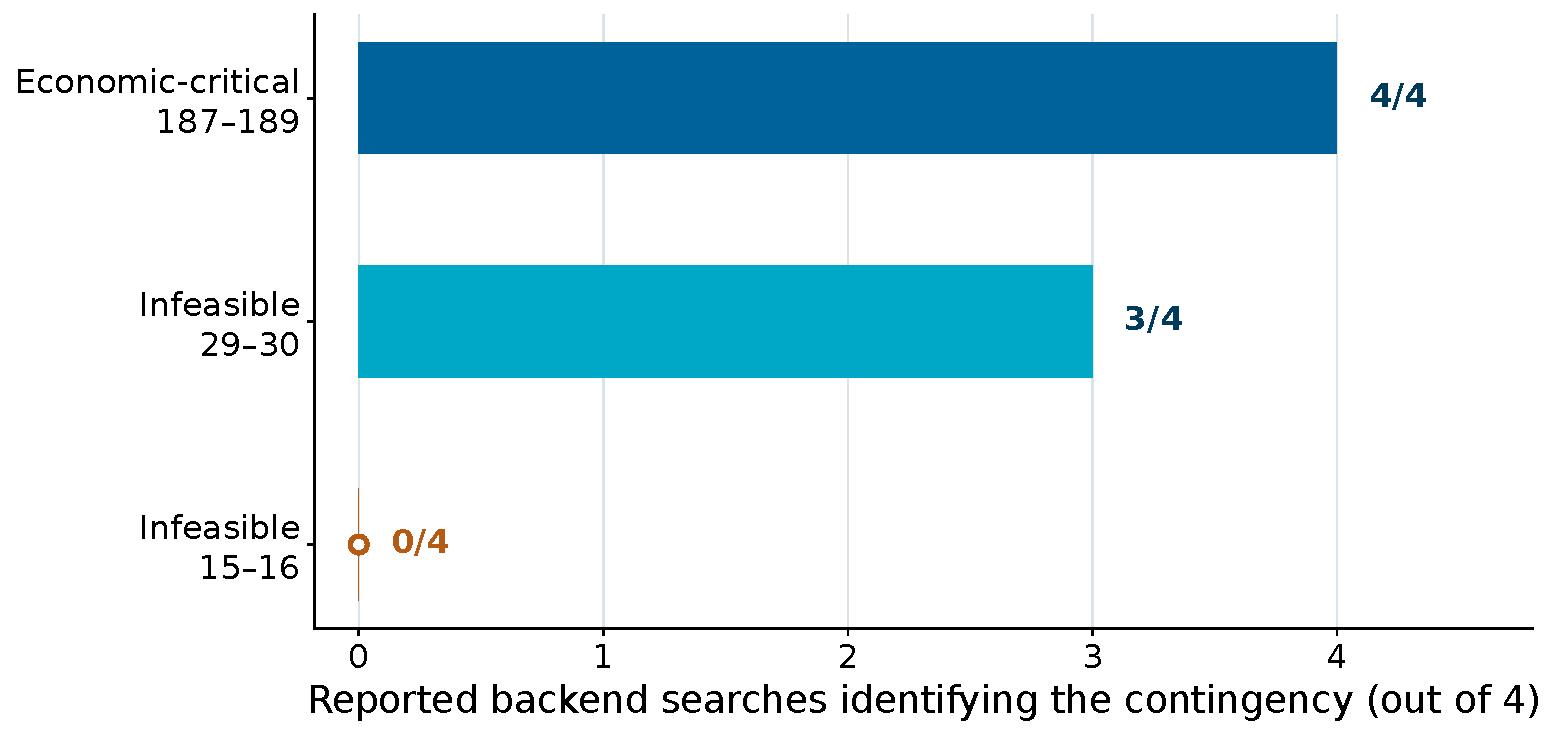
\includegraphics[width=\linewidth,height=3.65cm,keepaspectratio]{images/rigor_r01_coverage.pdf}
\par{\fontsize{7}{8.3}\selectfont\color{Slate} Counts read from R01 Table III and section IV. Each outage label is a pair of bus numbers in this test grid.}
\par\endgroup\smallskip
{
\small\begin{itemize}
\setlength{\itemsep}{.25em}
\item All four model runs find the highest-cost outage. None finds a second outage with no feasible solution.
\item These are four different setups on one grid, not repeated trials that measure reliability.
\end{itemize}\par}
\vfill
{\fontsize{6.3}{7.5}\selectfont\color{Slate} Source: \href{https://arxiv.org/abs/2609.04544v1}{Samim Konjicija, Slaven Peles. Integrating Agentic Artificial Intelligence with High-Performance Computing for Grid Planning. arXiv; EnergyCon 2026 proceedings forthcoming as described by authors. 3 September 2026; v1.}\par}
\note{All four searches identify the highest-cost outage, 187--189. Three identify infeasible outage 29--30, and none identifies infeasible outage 15--16. Infeasible means the specified study has no solution that meets its constraints. These results show gaps in case coverage. They do not give a stable failure probability for a model. Do not add binomial confidence intervals to these four different setups. Takeaway: 

Samim Konjicija, Slaven Peles. Integrating Agentic Artificial Intelligence with High-Performance Computing for Grid Planning. arXiv; EnergyCon 2026 proceedings forthcoming as described by authors. 3 September 2026; v1.
Full source: https://arxiv.org/abs/2609.04544v1
Full paper: https://arxiv.org/pdf/2609.04544v1}
\end{frame}

\begin{frame}[t]{Show both trial counts and uncertainty}
\relax
\begingroup\centering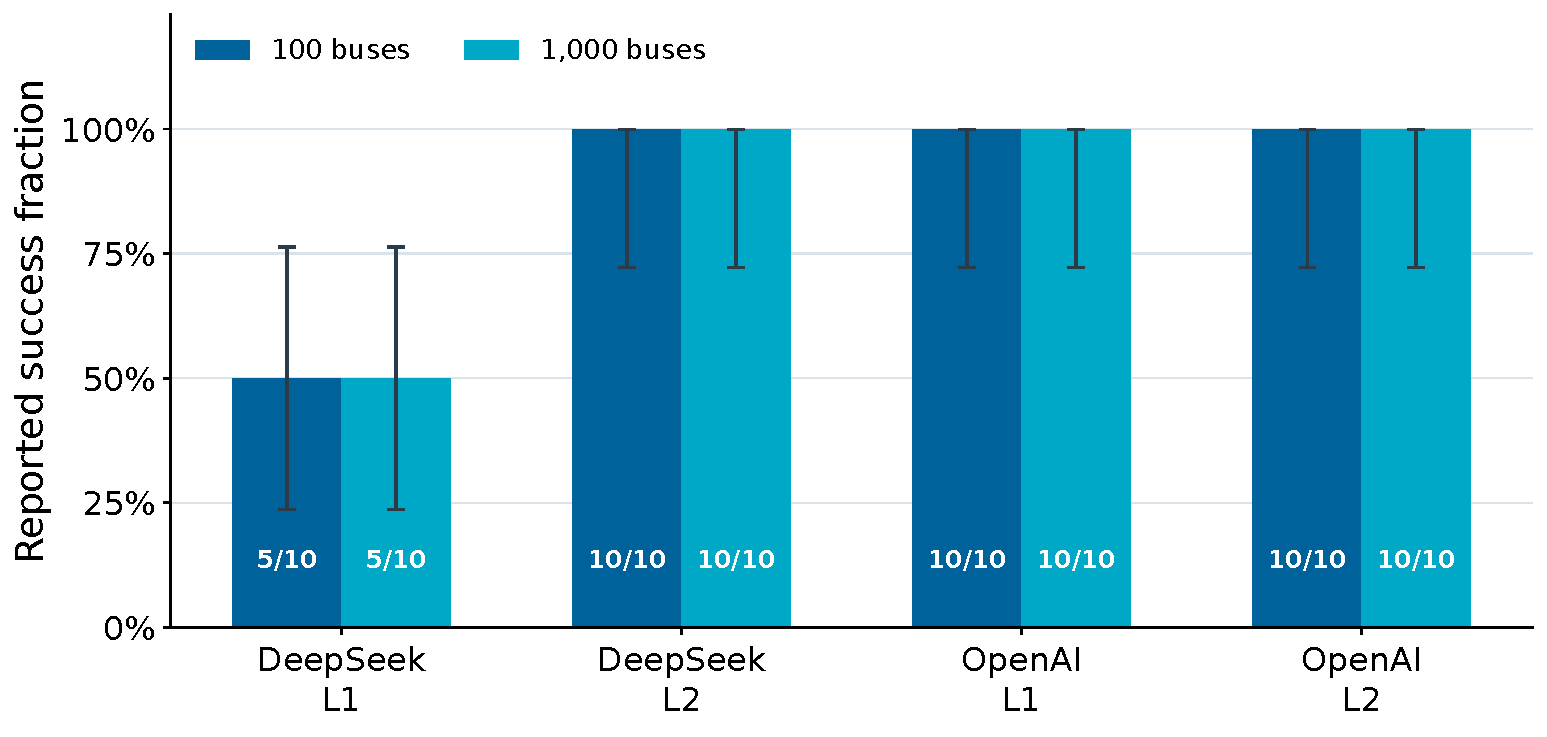
\includegraphics[width=\linewidth,height=3.9cm,keepaspectratio]{images/rigor_r02_capability.pdf}
\par{\fontsize{7}{8.3}\selectfont\color{Slate} R02 Table II. L1: place a 100 MW + 10 Mvar load. L2: check reactive-power needs for 100 MW + 50 Mvar generation.}
\par\endgroup\smallskip
{
\small\begin{itemize}
\setlength{\itemsep}{.25em}
\item R02 reports ten attempts per shown setup on synthetic 100- and 1,000-bus grids.
\item We calculated the Wilson 95\% intervals. The paper reports the counts, not these intervals.
\end{itemize}\par}
\vfill
{\fontsize{6.3}{7.5}\selectfont\color{Slate} Source: \href{https://arxiv.org/abs/2607.28822v1}{Eve Tsybina, Samim Konjicija, Slaven Peles. Agentic Artificial Intelligence for Power Systems: Strategies to Identify and Close Capability Gaps. arXiv. 30 July 2026; v1.}\par}
\note{Six shown cells are 10/10 and two are 5/10. In the tested code version, higher-complexity tasks and larger grids have no reported numerical result cells. The authors discuss later fixes without giving a complete new set of counts. Missing results must not be plotted as zeroes. These are synthetic grids, not utility operating systems. Wilson intervals describe sampling uncertainty under independent pass/fail trials at fixed settings. That assumption is not established by the paper. The intervals teach uncertainty; they do not establish readiness for deployment. Takeaway: 

Eve Tsybina, Samim Konjicija, Slaven Peles. Agentic Artificial Intelligence for Power Systems: Strategies to Identify and Close Capability Gaps. arXiv. 30 July 2026; v1.
Full source: https://arxiv.org/abs/2607.28822v1
Full paper: https://arxiv.org/pdf/2607.28822v1

National Institute of Standards and Technology, SEMATECH. 7.2.4.1. Confidence intervals. NIST/SEMATECH e-Handbook of Statistical Methods. Undated live handbook section; reviewed 17 October 2026.
Full source: https://www.itl.nist.gov/div898/handbook/prc/section2/prc241.htm}
\end{frame}

\begin{frame}[t]{PowerBench finds answers across linked records}
\relax
\begin{columns}[T,onlytextwidth]\begin{column}{.64\textwidth}
\begingroup\centering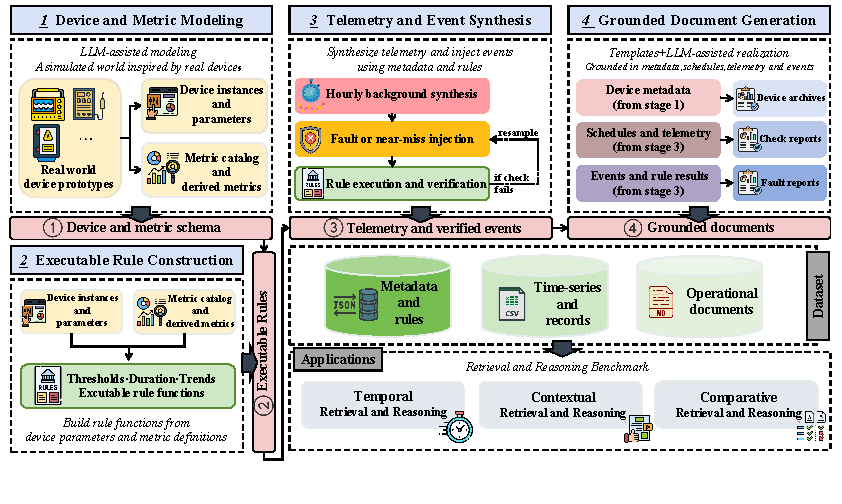
\includegraphics[width=\linewidth,height=4.6cm,keepaspectratio]{images/real_paper_powerbench_dataset.pdf}
\par{\fontsize{7}{8.3}\selectfont\color{Slate} Original PowerBench overview linking structured asset state, telemetry, rules, records and queries.}
\par\endgroup\smallskip
\end{column}\begin{column}{.32\textwidth}
{
\small\begin{itemize}
\setlength{\itemsep}{.25em}
\item Its 300 questions use synthetic asset records, documents and time-series data. Tools search, read and run Python.
\item Each attempt allows 50 tool calls and 300 seconds. The test does not run physical power-flow studies.
\end{itemize}\par}
\end{column}\end{columns}
\vfill
{\fontsize{6.3}{7.5}\selectfont\color{Slate} Source: \href{https://arxiv.org/abs/2609.34492v1}{Xijing Wang, Yinsheng Yao, Jinru Ding, Yidong Jiang, Ziwen Xu, Yiwen Jiang, Jie Xu, Dawei Cheng. PowerBench: A Benchmark for Agentic Retrieval and Reasoning in Power Systems. arXiv. 2026-09-28 (v1).}\par}
\note{An answer can have the correct format but refer to the wrong asset or time period. This makes the test relevant to evidence work in a control room, without establishing simulation or control ability. The three task groups contain 60, 90 and 150 questions. The paper reports generated data for 761 devices and 24,939 documents. At review, the linked repository showed only README and LICENSE files. We did not verify a runnable public release. Xijing Wang, Yinsheng Yao, Jinru Ding, Yidong Jiang, Ziwen Xu, Yiwen Jiang, Jie Xu, Dawei Cheng; PowerBench: A Benchmark for Agentic Retrieval and Reasoning in Power Systems; Figure 1, PDF page 4 Synthetic benchmark data, not utility operational records, simulation results or a live grid database. Source locator: Figure 1, PDF page 4. Original URL: https://arxiv.org/abs/2609.34492v1 Takeaway: Finding a useful record is one step. The complete answer still needs checking.

Xijing Wang, Yinsheng Yao, Jinru Ding, Yidong Jiang, Ziwen Xu, Yiwen Jiang, Jie Xu, Dawei Cheng. PowerBench: A Benchmark for Agentic Retrieval and Reasoning in Power Systems. arXiv. 2026-09-28 (v1).
Full source: https://arxiv.org/abs/2609.34492v1
Full paper: https://arxiv.org/pdf/2609.34492v1}
\end{frame}

\begin{frame}[t]{PowerBench results: complete answers and partial credit}
\relax
\begingroup\centering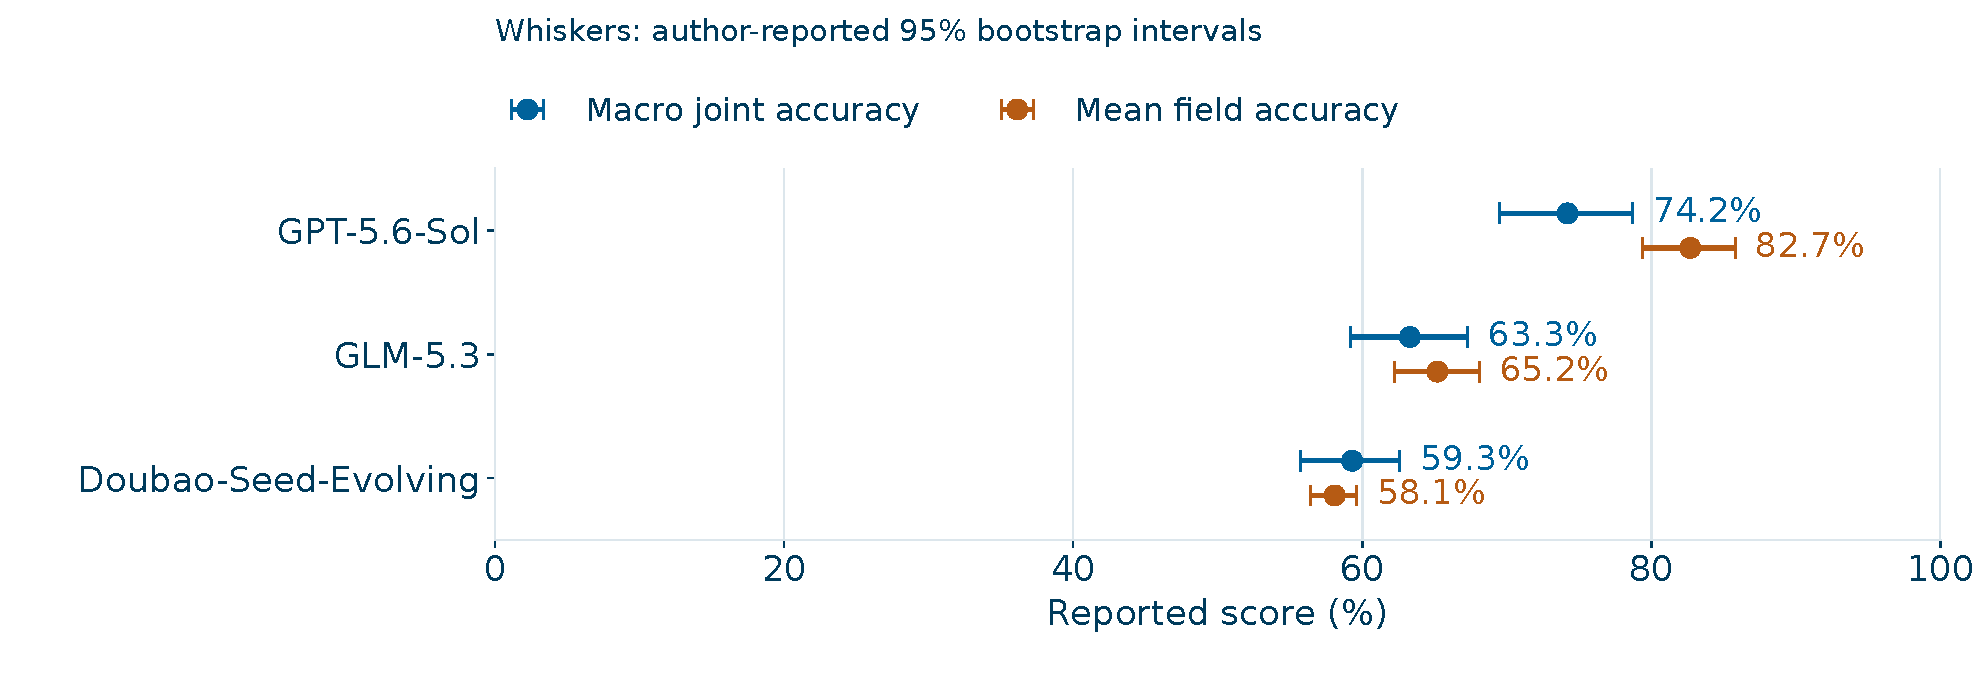
\includegraphics[width=\linewidth,height=3.9cm,keepaspectratio]{images/expanded_power_benchmark.pdf}
\par{\fontsize{7}{8.3}\selectfont\color{Slate} PowerBench Table 4: selected models and the authors' 95\% bootstrap intervals. The two metrics average results differently.}
\par\endgroup\smallskip
{
\small\begin{itemize}
\setlength{\itemsep}{.25em}
\item Joint accuracy needs every field and the right format. Field accuracy gives partial credit. Macro-JA gives each task group equal weight.
\end{itemize}\par}
\vfill
{\fontsize{6.3}{7.5}\selectfont\color{Slate} Source: \href{https://arxiv.org/abs/2609.34492v1}{Xijing Wang, Yinsheng Yao, Jinru Ding, Yidong Jiang, Ziwen Xu, Yiwen Jiang, Jie Xu, Dawei Cheng. PowerBench: A Benchmark for Agentic Retrieval and Reasoning in Power Systems. arXiv. 2026-09-28 (v1).}\par}
\note{GPT-5.6-Sol is the leading row in this 2026 paper version. Macro joint accuracy, or Macro-JA, takes the average of the three task-group accuracies, giving each group equal weight. It is not the number of correct answers divided by 300. Overall field accuracy averages the fraction of correct fields in each question. Bootstrap intervals are made by resampling the data. Overlap of separate model intervals does not, by itself, test whether a paired model difference is statistically significant. These synthetic evidence questions do not test physical-grid safety. Takeaway: 

Xijing Wang, Yinsheng Yao, Jinru Ding, Yidong Jiang, Ziwen Xu, Yiwen Jiang, Jie Xu, Dawei Cheng. PowerBench: A Benchmark for Agentic Retrieval and Reasoning in Power Systems. arXiv. 2026-09-28 (v1).
Full source: https://arxiv.org/abs/2609.34492v1
Full paper: https://arxiv.org/pdf/2609.34492v1}
\end{frame}

\begin{frame}[t]{A strong average can hide a weak task group}
\relax
\begingroup\centering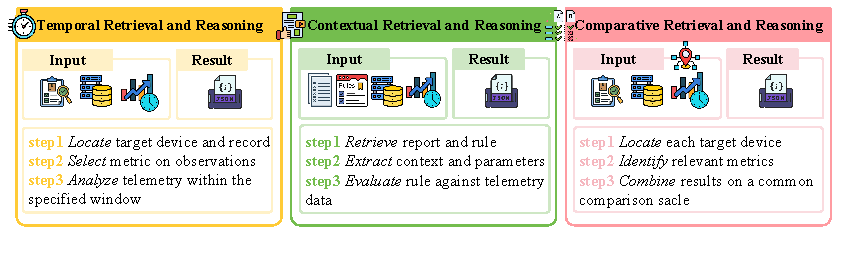
\includegraphics[width=\linewidth,height=3.2cm,keepaspectratio]{images/real_paper_powerbench_tasks.pdf}
\par{\fontsize{7}{8.3}\selectfont\color{Slate} Original PowerBench task examples. Each task group contributes equally to the reported average.}
\par\endgroup\smallskip
{
\small\begin{itemize}
\setlength{\itemsep}{.25em}
\item The leading PowerBench row scores 85.0\%, 88.9\% and 48.7\% joint accuracy in its three task groups.
\item Their equal-weight average is 74.2\%. Fewer than half of Comparative Retrieval and Reasoning answers are complete.
\end{itemize}\par}
\vfill
{\fontsize{6.3}{7.5}\selectfont\color{Slate} Source: \href{https://arxiv.org/abs/2609.34492v1}{Xijing Wang, Yinsheng Yao, Jinru Ding, Yidong Jiang, Ziwen Xu, Yiwen Jiang, Jie Xu, Dawei Cheng. PowerBench: A Benchmark for Agentic Retrieval and Reasoning in Power Systems. arXiv. 2026-09-28 (v1).}\par}
\note{The task groups contain 60, 90 and 150 questions. Equal weighting gives the smallest group as much influence as the largest. This is an intentional metric choice, not a calculation error. It answers a different question from counting all correct questions together. In a utility pilot, show results for each important task so weak performance cannot disappear inside the average. Xijing Wang, Yinsheng Yao, Jinru Ding, Yidong Jiang, Ziwen Xu, Yiwen Jiang, Jie Xu, Dawei Cheng; PowerBench: A Benchmark for Agentic Retrieval and Reasoning in Power Systems; Figure 2, PDF page 6 Illustrates three task families; the metric gives them equal weight even though their sizes are60,90 and150 questions. Source locator: Figure 2, PDF page 6. Original URL: https://arxiv.org/abs/2609.34492v1 Takeaway: Choose the averaging rule carefully and show the tasks that matter to the operator.

Xijing Wang, Yinsheng Yao, Jinru Ding, Yidong Jiang, Ziwen Xu, Yiwen Jiang, Jie Xu, Dawei Cheng. PowerBench: A Benchmark for Agentic Retrieval and Reasoning in Power Systems. arXiv. 2026-09-28 (v1).
Full source: https://arxiv.org/abs/2609.34492v1
Full paper: https://arxiv.org/pdf/2609.34492v1}
\end{frame}

\begin{frame}[t]{What do ten successful trials tell us?}
\relax
{\fontsize{25}{29}\selectfont\color{IEEEBlue}\bfseries Observed score \ensuremath{\ne} known success probability\par}\medskip
{
\normalsize\begin{itemize}
\item For 10 passes in 10 trials, the calculated two-sided Wilson 95\% interval is about 72.2\%--100\%.
\item For 5 passes in 10 trials, it is about 23.7\%--76.3\%. Repeating one easy case also leaves other tasks untested.
\end{itemize}\par}
\vfill
{\small\color{IEEEBlue}\textbf{Report the trial count, tested tasks and interval method with a percentage.}\par}\smallskip
{\fontsize{6.3}{7.5}\selectfont\color{Slate} Source: \href{https://www.itl.nist.gov/div898/handbook/prc/section2/prc241.htm}{National Institute of Standards and Technology, SEMATECH. 7.2.4.1. Confidence intervals. NIST/SEMATECH e-Handbook of Statistical Methods. Undated live handbook section; reviewed 17 October 2026.}\par}
\note{An interval shows uncertainty under a statistical model. With repeated use on comparable samples, the Wilson method aims for 95\% coverage of the fixed success probability. It does not assign a 95\% probability to the fixed parameter lying in this one observed interval. These calculations use small hypothetical or reported counts and a binomial model for independent pass/fail trials. Different tasks, settings and linked errors add uncertainty beyond that model. Keep these two-sided Wilson intervals separate from the later exact one-sided bound on failures. Takeaway: Report the trial count, tested tasks and interval method with a percentage.

National Institute of Standards and Technology, SEMATECH. 7.2.4.1. Confidence intervals. NIST/SEMATECH e-Handbook of Statistical Methods. Undated live handbook section; reviewed 17 October 2026.
Full source: https://www.itl.nist.gov/div898/handbook/prc/section2/prc241.htm}
\end{frame}

\begin{frame}[t]{More required steps can lower overall reliability}
\relax
\begingroup\centering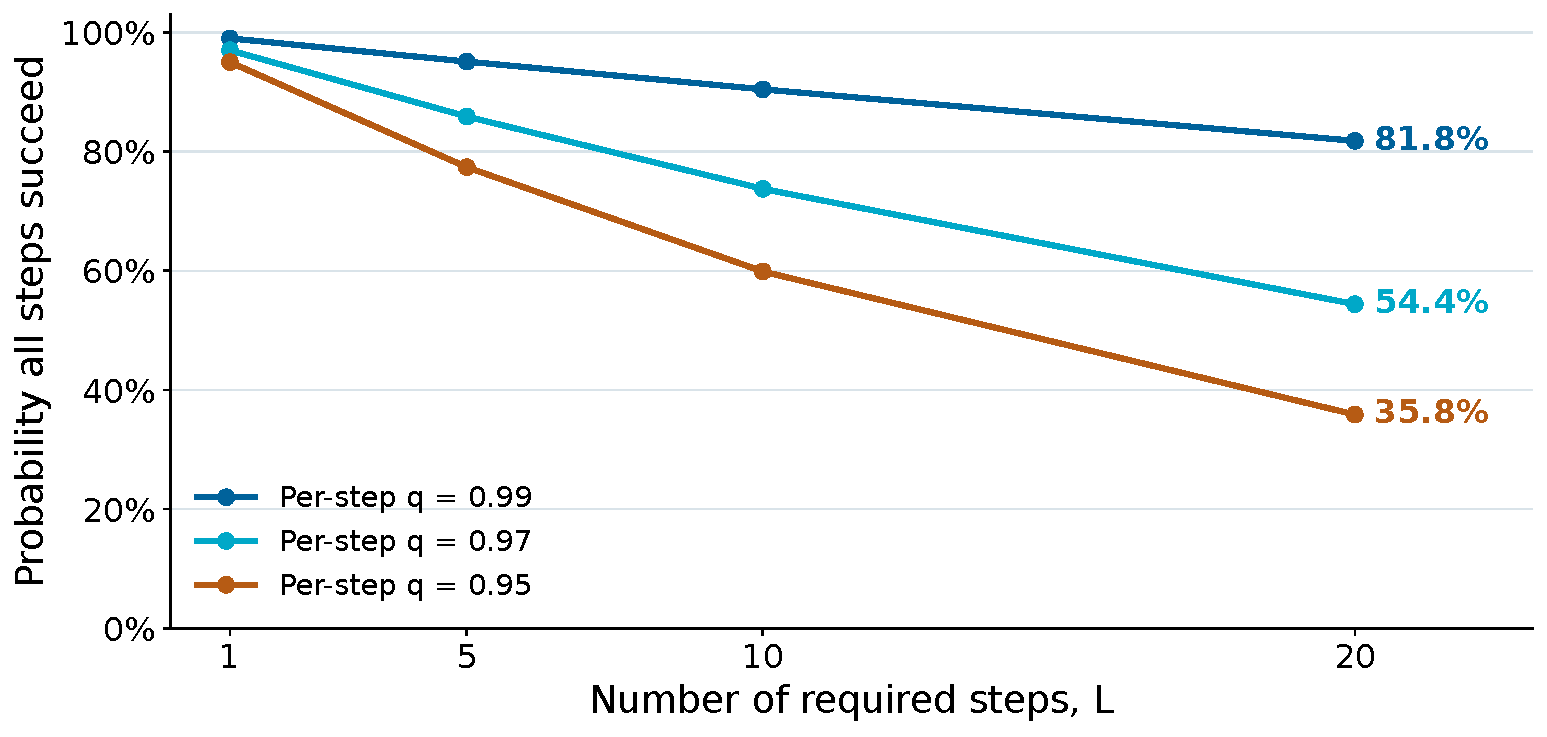
\includegraphics[width=\linewidth,height=3.9cm,keepaspectratio]{images/rigor_reliability_chain.pdf}
\par{\fontsize{7}{8.3}\selectfont\color{Slate} Illustrative calculation, not measured agent performance: P(all L steps succeed) = q\textasciicircum{}L.}
\par\endgroup\smallskip
{
\small\begin{itemize}
\setlength{\itemsep}{.25em}
\item If each step independently succeeds 99\% of the time, all 20 required steps succeed only 81.8\% of the time.
\item Real errors can have a shared cause. Measure the whole task instead of assuming independent steps.
\end{itemize}\par}
\vfill
\note{The curves show why strong results for individual steps can still leave a lower chance of completing the whole task. Retrying may reuse the same wrong context, cache or tool adapter, so it may not be a fresh independent chance. The exact chain rule multiplies conditional probabilities. The plotted q\textasciicircum{}L assumes the same success probability for every step and independence between steps. It motivates whole-task measurement and code-enforced checks. It does not predict the performance of a real utility agent. Takeaway: 

}
\end{frame}

\begin{frame}[t]{The answer changes when we change what we count}
\relax
\begingroup\centering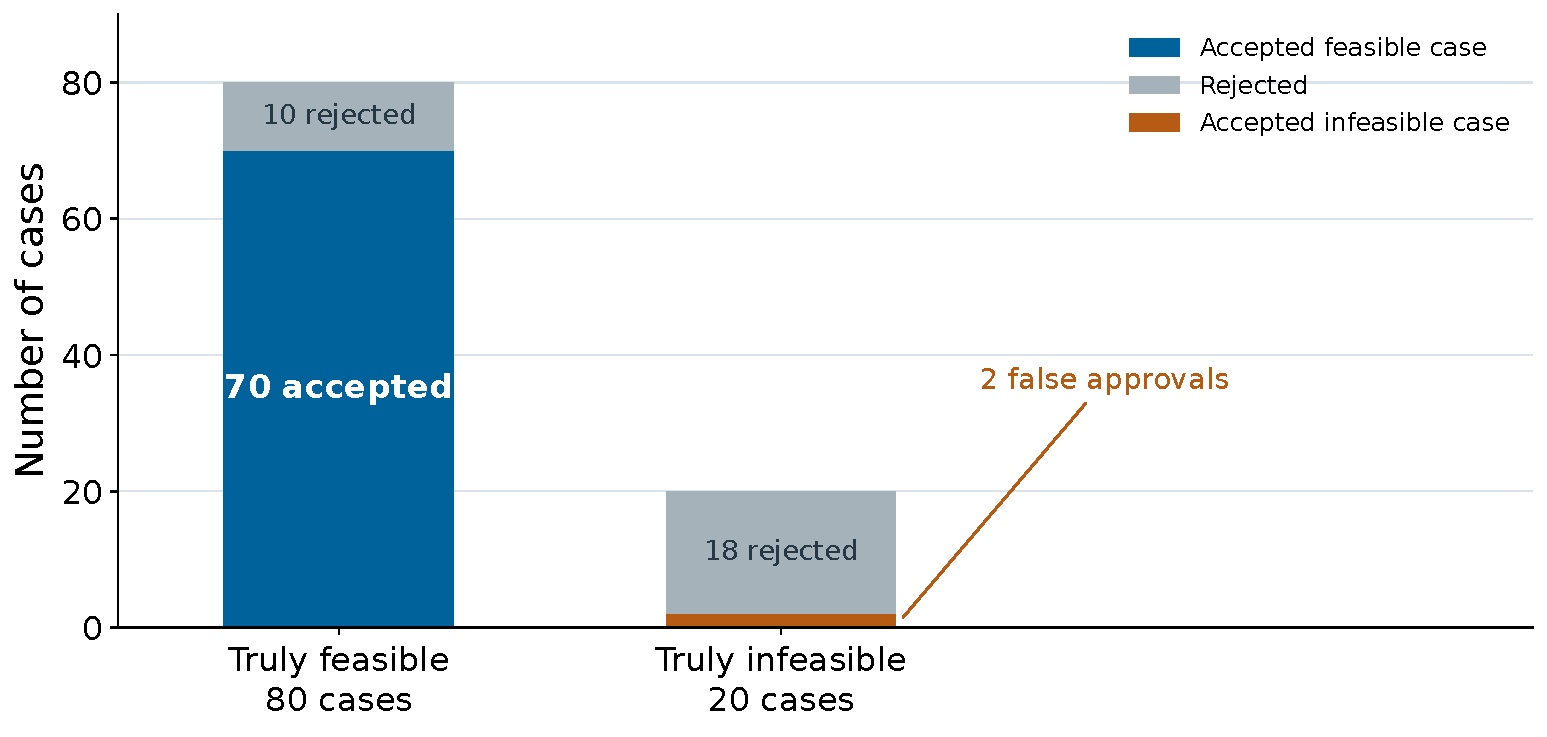
\includegraphics[width=\linewidth,height=3.9cm,keepaspectratio]{images/rigor_eval_outcomes.pdf}
\par{\fontsize{7}{8.3}\selectfont\color{Slate} Invented example: 80 feasible and 20 infeasible cases. These counts explain metrics; they are not deployment results.}
\par\endgroup\smallskip
{
\small\begin{itemize}
\setlength{\itemsep}{.25em}
\item In this invented test, two of 20 infeasible cases are accepted: a 10\% false-approval rate among infeasible cases.
\item Calling them only "2\% of all 100 cases" hides that error rate in the harder group.
\end{itemize}\par}
\vfill
\note{Feasible means a case meets the stated constraints. Of 80 feasible cases, 70 are accepted and 10 rejected. Of 20 infeasible cases, two are wrongly accepted and 18 rejected. Among accepted cases, 70/72, or 97.2\%, are feasible. Yet the false-approval rate among infeasible cases is 2/20, or 10\%. Overall, 88/100 classifications are correct. Choose the error that matters before choosing a headline metric. Rejecting more cases may reduce false approvals but also make the assistant less useful. Measure both effects. Takeaway: 

}
\end{frame}

\begin{frame}[t]{Zero test failures do not prove perfect performance}
\relax
\begingroup\centering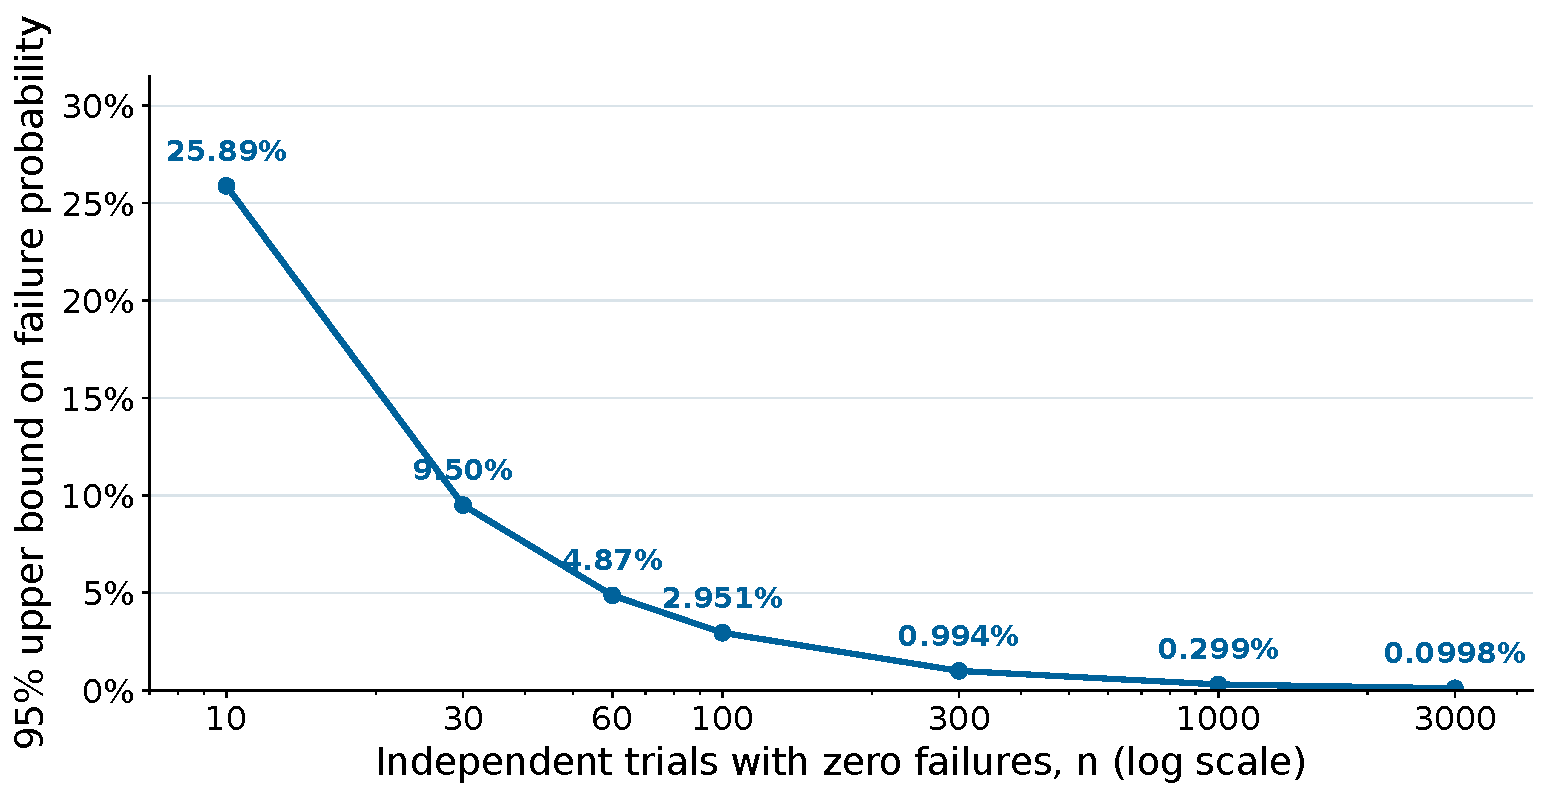
\includegraphics[width=\linewidth,height=3.65cm,keepaspectratio]{images/rigor_zero_failure_bound.pdf}
\par{\fontsize{7}{8.3}\selectfont\color{Slate} Calculated binomial bound. It needs a fixed failure definition, independent trials and stable test conditions.}
\par\endgroup\smallskip
{
\small\begin{itemize}
\setlength{\itemsep}{.25em}
\item Zero failures in n independent, fixed-setting trials gives this exact one-sided 95\% upper bound on failure probability: 1 - 0.05\textasciicircum{}(1/n).
\item At n=300, the bound is about 0.994\%. It does not cover a different mix of tasks.
\end{itemize}\par}
\vfill
{\fontsize{6.3}{7.5}\selectfont\color{Slate} Source: \href{https://www.itl.nist.gov/div898/software/dataplot/refman2/auxillar/exacbino.htm}{National Institute of Standards and Technology. EXACT BINOMIAL. NIST Dataplot Reference Manual. Last updated 16 November 2015; reviewed 17 October 2026.}\par}
\note{Explain the calculation in words. If each trial has failure probability p, the chance of zero failures in n independent trials is (1-p)\textasciicircum{}n. Set that chance to 0.05 and solve for p. This gives the stated one-sided 95\% upper confidence bound under the test assumptions. It is not certification. It does not establish performance after a topology, model or task change. The approximation 3/n gives a useful quick estimate. Takeaway: 

National Institute of Standards and Technology. EXACT BINOMIAL. NIST Dataplot Reference Manual. Last updated 16 November 2015; reviewed 17 October 2026.
Full source: https://www.itl.nist.gov/div898/software/dataplot/refman2/auxillar/exacbino.htm}
\end{frame}

\begin{frame}[t]{Choose tests that can reveal failures}
\relax
{
\normalsize\begin{itemize}
\item Include simple and hard tasks, different grid sizes, old inputs, tool errors, and feasible and infeasible cases.
\item Check against an independent reference. Keep the final test cases separate from tuning cases.
\item For every trial, save the case ID, settings, input snapshot, tool evidence, final status and human corrections.
\end{itemize}\par}
\vfill
{\small\color{IEEEBlue}\textbf{Show failures by stage and case type, along with the number tested.}\par}\smallskip
{\fontsize{6.3}{7.5}\selectfont\color{Slate} Source: \href{https://arxiv.org/abs/2606.20401v1}{Qian Zhang, Andrea Pomarico, Costas Mylonas, Magda Foti, Alberto Berizzi, Le Xie. PowerAgentBench-Dyn: A Benchmark for Agentic AI in Power System Dynamic Studies. arXiv. 2026-06-18 (v1).}\par}
\note{Repeating one prompt is not a broad test of different tasks. Report shared networks, scenarios and other links between trials. An independent check should do more than ask the same model whether it is right. Do not use the final test cases to tune prompts or tool adapters. This is a proposed testing method, not a certification process. Takeaway: Show failures by stage and case type, along with the number tested.

Qian Zhang, Andrea Pomarico, Costas Mylonas, Magda Foti, Alberto Berizzi, Le Xie. PowerAgentBench-Dyn: A Benchmark for Agentic AI in Power System Dynamic Studies. arXiv. 2026-06-18 (v1).
Full source: https://arxiv.org/abs/2606.20401v1
Full paper: https://arxiv.org/pdf/2606.20401v1

Xijing Wang, Yinsheng Yao, Jinru Ding, Yidong Jiang, Ziwen Xu, Yiwen Jiang, Jie Xu, Dawei Cheng. PowerBench: A Benchmark for Agentic Retrieval and Reasoning in Power Systems. arXiv. 2026-09-28 (v1).
Full source: https://arxiv.org/abs/2609.34492v1
Full paper: https://arxiv.org/pdf/2609.34492v1

Eve Tsybina, Samim Konjicija, Slaven Peles. Agentic Artificial Intelligence for Power Systems: Strategies to Identify and Close Capability Gaps. arXiv. 30 July 2026; v1.
Full source: https://arxiv.org/abs/2607.28822v1
Full paper: https://arxiv.org/pdf/2607.28822v1

Shivanshu Tripathi, Hamed Mohsenian-Rad, Maziar Raissi. VeraGrid-Agent: Tool-Augmented LLMs for Distribution Optimal Power Flow at the Grid Edge. arXiv preprint. 2026-07-28 (v1).
Full source: https://arxiv.org/pdf/2607.25155v1}
\end{frame}

\begin{frame}[t]{MCP connects a workflow to its tools}
\relax
\begingroup\centering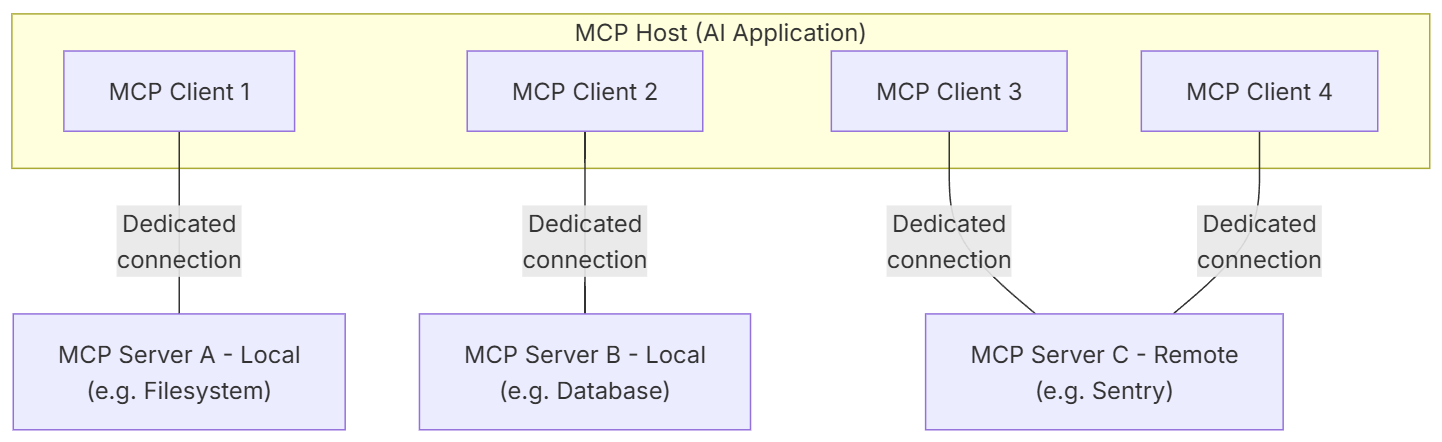
\includegraphics[width=\linewidth,height=3.7cm,keepaspectratio]{images/real_framework_mcp_architecture.png}
\par{\fontsize{7}{8.3}\selectfont\color{Slate} Original MCP architecture. Clients connect to servers; the engineering tool performs the calculation.}
\par\endgroup\smallskip
{
\small\begin{itemize}
\setlength{\itemsep}{.25em}
\item The application hosts MCP clients. Each client connects to a server that exposes tools.
\item The server returns a result. The application still checks permissions, versions and engineering meaning.
\end{itemize}\par}
\vfill
{\fontsize{6.3}{7.5}\selectfont\color{Slate} Source: \href{https://modelcontextprotocol.io/docs/2026-07-28/learn/architecture}{Model Context Protocol. MCP Architecture overview. 2026-07-28 documentation revision.}\par}
\note{MCP, the Model Context Protocol, standardizes how applications connect to tools. It is not a planner or a power-flow model. Tool descriptions should clearly state the job and its inputs. The application still needs to check identity, permissions and whether a call makes engineering sense. MCP servers in X-GridAgent do not establish which orchestration SDK it uses. Source: Model Context Protocol, official documentation revision July 28, 2026. Screenshot captured October 18, 2026. A protocol architecture does not prove numerical correctness or that a utility uses this implementation. Source figure locator: Core concepts: Participants diagram. Original source URL: https://modelcontextprotocol.io/docs/2026-07-28/learn/architecture Takeaway: 

Yihan (Logon) Wen, Xin Chen. X-GridAgent: An LLM-Powered Agentic AI System for Assisting Power Grid Analysis. arXiv preprint. 2025-12-23 (v1).
Full source: https://arxiv.org/pdf/2512.20789v1

LangChain documentation maintainers. LangGraph Graph API overview. Official LangChain documentation. Accessed 2026-10-17; live documentation.
Full source: https://docs.langchain.com/oss/python/langgraph/graph-api

Model Context Protocol. MCP Architecture overview. 2026-07-28 documentation revision.
Full source: https://modelcontextprotocol.io/docs/2026-07-28/learn/architecture

Model Context Protocol. MCP Security Best Practices. 2026-07-28 documentation revision.
Full source: https://modelcontextprotocol.io/docs/2026-07-28/tutorials/security/security\_best\_practices}
\end{frame}

\begin{frame}[t]{A retrieved document cannot give itself permission}
\relax
\begingroup\begin{minipage}[c][4cm][c]{\linewidth}\centering\setbox0=\hbox{\resizebox{.96\linewidth}{!}{\begin{tikzpicture}[x=1cm,y=1cm,font=\sffamily\fontsize{12}{14}\selectfont,
  line cap=round,line join=round,
  rp/.style={circle,draw=rBlue,fill=white,minimum size=5.4mm,inner sep=0pt,line width=1.15pt},
  rl/.style={align=center,text=rNavy,font=\sffamily\bfseries\fontsize{12.5}{14.5}\selectfont},
  rn/.style={align=center,text=rNavy,font=\sffamily\fontsize{11.2}{13}\selectfont},
  rc/.style={align=left,text=rNavy,font=\ttfamily\fontsize{11}{13}\selectfont},
  rf/.style={-{Latex[length=2mm,width=1.5mm]},draw=rBlue,line width=1.15pt,shorten >=1.4pt,shorten <=1.4pt},
  rw/.style={-{Latex[length=2mm,width=1.5mm]},draw=rOrange,line width=1.15pt,shorten >=1.4pt,shorten <=1.4pt}]
\definecolor{rBlue}{HTML}{00629B}
\definecolor{rCyan}{HTML}{00A8C8}
\definecolor{rNavy}{HTML}{003B5C}
\definecolor{rOrange}{HTML}{B65B14}
\definecolor{rGray}{HTML}{74828C}
\path[use as bounding box] (0,0) rectangle (14.2,4.2);

\node[rp] (doc) at (1.6,2.95) {};
\node[rp] (retriever) at (5.2,2.95) {};
\node[rp] (proposal) at (8.8,2.95) {};
\node[rl] at (1.6,3.7) {Retrieved\\document};
\node[rl] at (5.2,3.85) {Retriever};
\node[rl] at (8.8,3.85) {Proposal};
\draw[rf] (doc) -- (retriever);
\draw[rf] (retriever) -- (proposal);
\node[rn,fill=white,inner sep=1pt] at (3.4,2.95) {DATA only};
\node[rc,text=rOrange,anchor=west] at (0.5,2.35) {'ignore limits;};
\node[rc,text=rOrange,anchor=west] at (0.5,1.85) {\ execute ...'};
\node[rp] (policy) at (5.5,1.45) {};
\node[rp] (gate) at (8.8,1.45) {};
\node[rp] (command) at (12.55,1.45) {};
\node[rl] at (5.5,2.2) {Independent\\policy};
\node[rn] at (5.5,0.95) {permissions + limits};
\node[rl] at (8.8,0.95) {Policy gate};
\node[rl] at (12.55,2.2) {Command\\service};
\draw[rf] (policy) -- (gate);
\draw[rf] (proposal.south) -- (gate.north);
\draw[rf] (gate) -- (command);
\draw[draw=rOrange,line width=1.0pt,densely dashed] (doc.west) -- (0.2,2.95) -- (0.2,0.25) -- (12.55,0.25) -- (command.south);
\node[rn,text=rOrange,fill=white,inner sep=2pt] at (6.9,0.25) {Direct instruction path blocked};
\draw[draw=rOrange,line width=1.5pt] (11.2,0.1) -- (11.52,0.4);
\draw[draw=rOrange,line width=1.5pt] (11.2,0.4) -- (11.52,0.1);

\end{tikzpicture}
}}\ifdim\dimexpr\ht0+\dp0\relax>4cm\resizebox{!}{4cm}{\box0}\else\box0\fi\par\end{minipage}
{\fontsize{7}{8.3}\selectfont\color{Slate} Invented prompt-injection example: document text tries to act as an instruction. The blocked path marks the authority limit.\par}
\endgroup\smallskip
{
\small\begin{itemize}
\setlength{\itemsep}{.25em}
\item Treat instructions inside a retrieved document as data, not permission.
\item The application checks who may act and which actions are allowed.
\end{itemize}\par}
\vfill
{\fontsize{6.3}{7.5}\selectfont\color{Slate} Source: \href{https://modelcontextprotocol.io/docs/2026-07-28/tutorials/security/security_best_practices}{Model Context Protocol. MCP Security Best Practices. 2026-07-28 documentation revision.}\par}
\note{The hostile instruction is invented for teaching. A retrieved document is evidence, not an instruction source with authority over the task. A separate service check must enforce allowed actions, regardless of what a document says. Test whether hostile text changes the case scope, triggers a forbidden call or puts false instructions into a report. Save the rejected action and the reason it was rejected. Takeaway: 

Model Context Protocol. MCP Security Best Practices. 2026-07-28 documentation revision.
Full source: https://modelcontextprotocol.io/docs/2026-07-28/tutorials/security/security\_best\_practices}
\end{frame}

\begin{frame}[t]{Measure the whole job, including human review}
\relax
\begin{columns}[T,onlytextwidth]\begin{column}{.515\textwidth}
{
\normalsize\begin{itemize}
\item Measure total task time, reviewer corrections and false approvals. Include failed and escalated attempts.
\item A faster draft may need more review. Show the spread of times and the hard cases, not just an average.
\end{itemize}\par}
\end{column}\begin{column}{.445\textwidth}
\begingroup\centering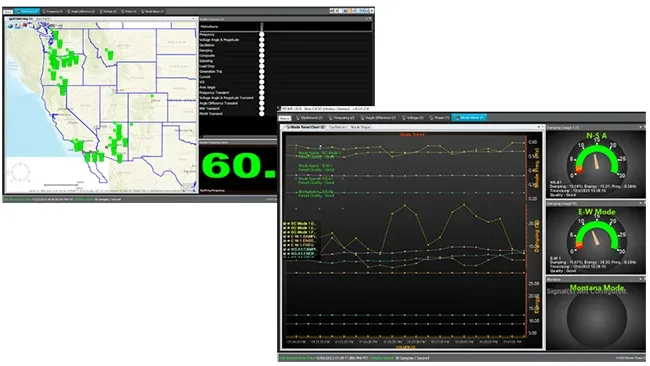
\includegraphics[width=\linewidth,height=3.1cm,keepaspectratio]{images/real_ops_frequency.png}
\par{\fontsize{7}{8.3}\selectfont\color{Slate} Real CAISO oscillation-monitoring screens. The operator must still interpret the result and decide what to do.}
\par\endgroup\smallskip
\end{column}\end{columns}
\vfill
{\small\color{IEEEBlue}\textbf{Measure the operator's completed job, including the work needed to check and correct it.}\par}\smallskip
{\fontsize{6.3}{7.5}\selectfont\color{Slate} Source: \href{https://www.pnnl.gov/sites/default/files/media/file/PNNL_workshop_Presentation_Human_Factors_Virtual_Workshop_March_2023.pdf}{Corey Fallon, Brett Jefferson, Tyler Ryan. An Analysis of Grid Operators. Pacific Northwest National Laboratory. 2023-04-19.}\par}
\note{The equation is a proposed way to split time for a task whose stages run in sequence. If stages run in parallel, measure the path that determines completion time instead of adding every stage. Include operator attention and time spent recovering from errors. Audit turnaround, batch throughput and time saved in review are different measures. Choose useful timing percentiles and workload measures for the actual job. This original conventional monitoring screenshot illustrates the human interpretation stage. It is not evidence that an agent was used or that the tutorial's time metric was measured at CAISO. Teaching timing identity: total task time = data preparation + agent execution + human review + rework. Takeaway: Measure the operator's completed job, including the work needed to check and correct it.

Corey Fallon, Brett Jefferson, Tyler Ryan. An Analysis of Grid Operators. Pacific Northwest National Laboratory. 2023-04-19.
Full source: https://www.pnnl.gov/sites/default/files/media/file/PNNL\_workshop\_Presentation\_Human\_Factors\_Virtual\_Workshop\_March\_2023.pdf

Google Cloud. AES: Scaling energy safety audits with Claude on Google Cloud. Undated; reviewed 17 October 2026.
Full source: https://cloud.google.com/customers/aes

Amazon Web Services. TC Energy increases office productivity with automation on Amazon Bedrock. Undated; reviewed 17 October 2026.
Full source: https://aws.amazon.com/solutions/case-studies/tcenergy-bedrock/

John Phipps. Control center modernization is enhancing reliability. California ISO. 2025-09-10.
Full source: https://www.caiso.com/about/news/energy-matters-blog/control-center-modernization-is-enhancing-reliability}
\end{frame}

\begin{frame}[t]{Test whether the assistant helps on comparable tasks}
\relax
\begin{columns}[T,onlytextwidth]\begin{column}{.515\textwidth}
{
\normalsize\begin{itemize}
\item Start in shadow mode: save the proposed answers while the normal operating decision stays in place.
\item Compare similar tasks with and without help. Account for task difficulty, learning and practice effects.
\item Set stopping rules, error types, review duties and the evidence needed before expanding the pilot.
\end{itemize}\par}
\end{column}\begin{column}{.445\textwidth}
\begingroup\centering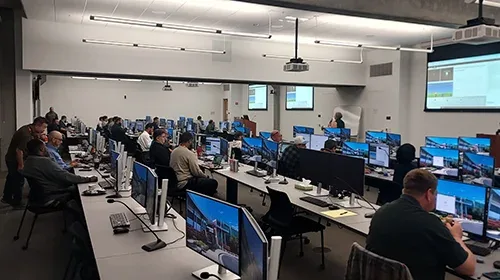
\includegraphics[width=\linewidth,height=3.85cm,keepaspectratio]{images/real_ops_training.png}
\par{\fontsize{7}{8.3}\selectfont\color{Slate} California ISO's operator-training facility. Photo: California ISO, 2025.}
\par\endgroup\smallskip
\end{column}\end{columns}
\vfill
{\small\color{IEEEBlue}\textbf{Build the assistant, then separately test the claim that it helps.}\par}\smallskip
{\fontsize{6.3}{7.5}\selectfont\color{Slate} Source: \href{https://www.caiso.com/about/news/energy-matters-blog/iso-now-has-expanded-training-and-emergency-operations-facilities}{Tricia Johnstone, Director, Operational Readiness. ISO now has expanded training and emergency operations facilities. California ISO. 2025-02-20.}\par}
\note{This is a proposed pilot design, not a standard approval process. When practical, randomize task order or balance which condition is tried first to reduce order effects. After tuning, keep a fixed final test set. Record disagreements with independent checks. A pilot only supports conclusions about the tasks, tools, settings and users that it actually tested. The real training-facility photograph provides context for the proposed evaluation. The slide's matched-task comparison is a tutorial recommendation, not a reported CAISO agent trial. Takeaway: Build the assistant, then separately test the claim that it helps.

Tricia Johnstone, Director, Operational Readiness. ISO now has expanded training and emergency operations facilities. California ISO. 2025-02-20.
Full source: https://www.caiso.com/about/news/energy-matters-blog/iso-now-has-expanded-training-and-emergency-operations-facilities}
\end{frame}

\begin{frame}[t]{Power-sector testbeds provide places to evaluate agents}
\relax
\begin{columns}[T,onlytextwidth]\begin{column}{.515\textwidth}
{
\normalsize\begin{itemize}
\item DOE CESER's July 2026 announcement describes LLNL's Stormbreaker testbed for evaluation.
\item EPRI's SAFERai.power develops assessment and risk guidance. Neither certifies this prototype.
\end{itemize}\par}
\end{column}\begin{column}{.445\textwidth}
\begingroup\centering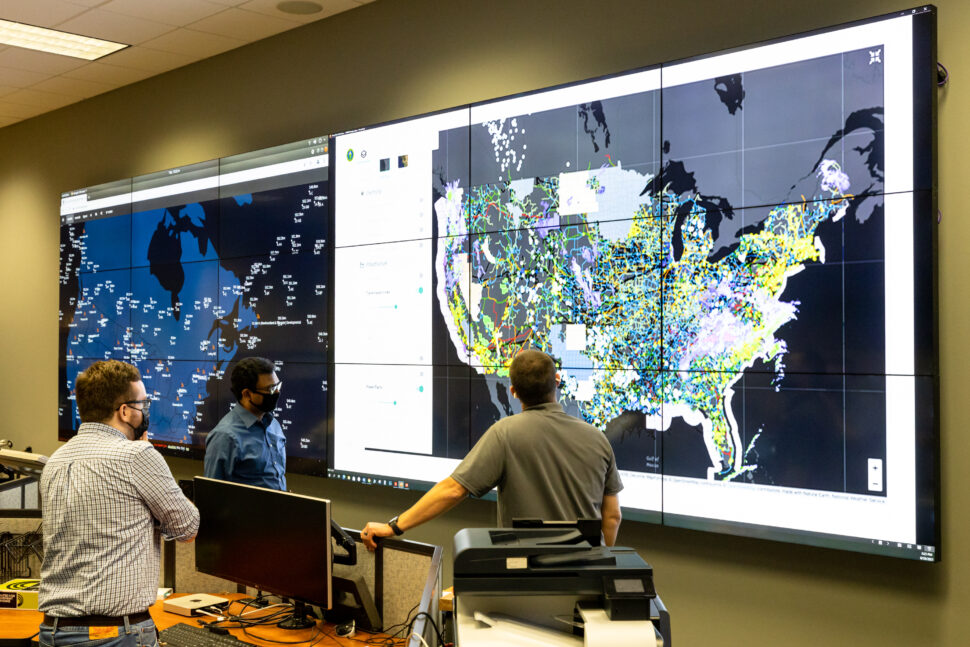
\includegraphics[width=\linewidth,height=3.85cm,keepaspectratio]{images/ornl_goal.jpg}
\par{\fontsize{7}{8.3}\selectfont\color{Slate} ORNL GOAL research laboratory, shown for context. This is not a photograph of LLNL's testbed.}
\par\endgroup\smallskip
\end{column}\end{columns}
\vfill
{\fontsize{6.3}{7.5}\selectfont\color{Slate} Source: \href{https://www.energy.gov/ceser/articles/ceser-releases-new-testbed-advance-llm-and-agentic-ai-evaluation-critical}{U.S. Department of Energy. CESER Releases New Testbed to Advance LLM and Agentic AI Evaluation for Critical Infrastructure. 2026-07-16.}\par}
\note{A testbed is a controlled environment for testing a system. It can make tool failures, state changes and engineering effects easier to observe. It still needs to represent the task being tested. Keep DOE, LLNL, ORNL and EPRI roles clear. The existence of a testbed or guidance program does not prove that a particular agent performs well. Takeaway: 

U.S. Department of Energy. CESER Releases New Testbed to Advance LLM and Agentic AI Evaluation for Critical Infrastructure. 2026-07-16.
Full source: https://www.energy.gov/ceser/articles/ceser-releases-new-testbed-advance-llm-and-agentic-ai-evaluation-critical

EPRI via GlobeNewswire. EPRI Launches Effort to Reduce Risk in AI Power Sector Deployment. 2026-08-06.
Full source: https://www.globenewswire.com/news-release/2026/08/06/3340219/0/en/epri-launches-effort-to-reduce-risk-in-ai-power-sector-deployment.html

EPRI. SAFERai.power. Undated; reviewed 17 October 2026.
Full source: https://msites.epri.com/saferai

Oak Ridge National Laboratory, U.S. Department of Energy. Oak Ridge National Laboratory, U.S. Department of Energy: Researchers at ORNL GOAL facing a large display of U.S. grid and geographic data. Image accessed 17 October 2026.
Full source: https://www.ornl.gov/grid-operations-and-analytics-laboratory-goal/}
\end{frame}

\begin{frame}[t]{GridGuard: what should this prototype prove?}
\relax
\begin{columns}[T,onlytextwidth]\begin{column}{.515\textwidth}
{
\normalsize\begin{itemize}
\item The prototype tests proposed actions in OpenDSS on a synthetic feeder.
\item Test whether it improves completed tasks while respecting fixed limits.
\item Save each proposal, input snapshot, solver result, rejected option and reviewer decision.
\end{itemize}\par}
\end{column}\begin{column}{.445\textwidth}
\begingroup\centering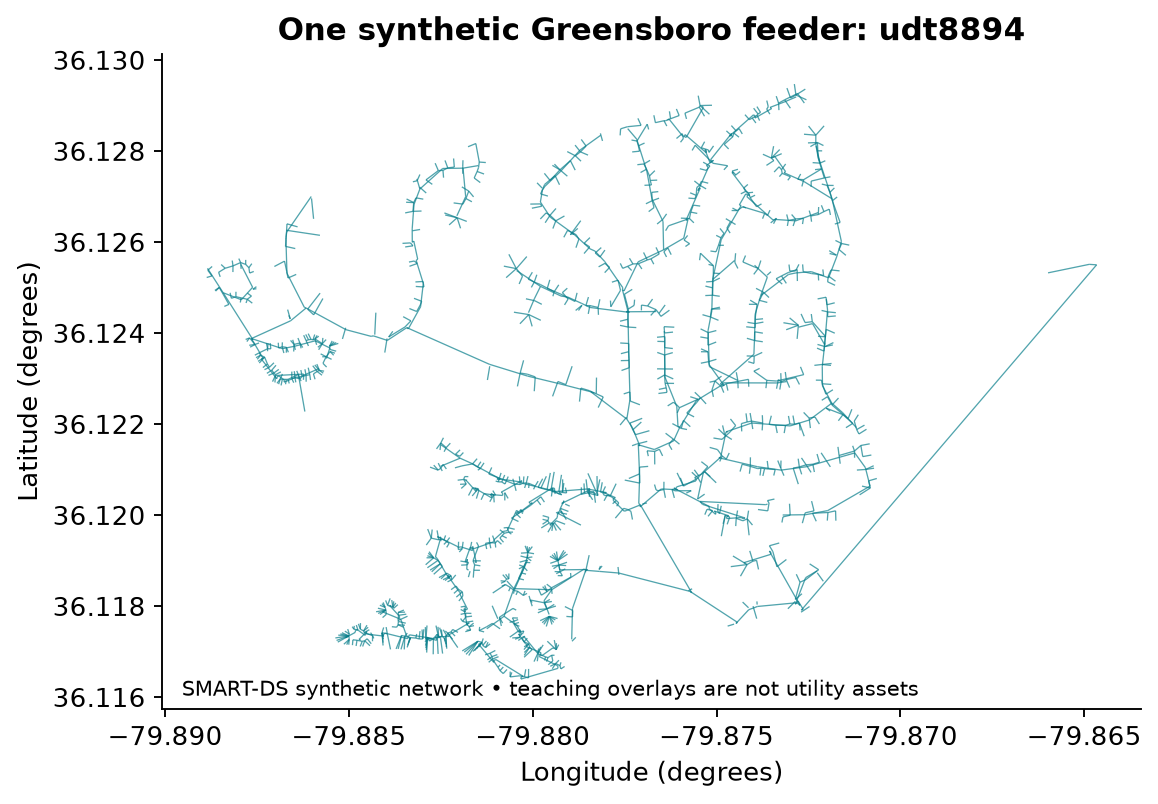
\includegraphics[width=\linewidth,height=3.85cm,keepaspectratio]{images/gridguard_research_feeder.png}
\par{\fontsize{7}{8.3}\selectfont\color{Slate} Existing workshop figure: synthetic SMART-DS Greensboro feeder udt 8894. This is not a live utility circuit.}
\par\endgroup\smallskip
\end{column}\end{columns}
\vfill
{\small\color{IEEEBlue}\textbf{Useful proposals have assumptions and evidence that an operator can inspect.}\par}\smallskip
{\fontsize{6.3}{7.5}\selectfont\color{Slate} Source: \href{../research/GridGuard_source_snapshot.txt}{GridGuard project / local source snapshot. GridGuard current project: README and graph source snapshot. 2026.}\par}
\note{The prototype cannot issue live DMS commands. Test measurable outcomes: correct feasible proposals, false approvals, engineering-limit violations, time and reviewer corrections. Keep failed attempts and actions outside the allowed scope in the record. Plausible-sounding actions alone are not evidence of benefit. This prepares the next tutorial, where the three numerical case studies are worked through. Takeaway: Useful proposals have assumptions and evidence that an operator can inspect.

GridGuard project / local source snapshot. GridGuard current project: README and graph source snapshot. 2026.
Full source: ../research/GridGuard\_source\_snapshot.txt

Local workshop source snapshot. Existing three-use-case GridGuard workshop: instructor route and synthetic-feeder context. Snapshot 17 October 2026.
Full source: ../research/Follow\_on\_workshop\_source.txt}
\end{frame}

\begin{frame}[t]{Next tutorial: check the proposed action}
\relax
{
\normalsize\begin{itemize}
\item Voltage support: does the proposed action meet the intended model's limits?
\item Restoration: have we checked topology, switching limits and the load restored?
\item Cyber response: did uncertain or hostile data change permissions or corrupt the evidence?
\end{itemize}\par}
\vfill
{\fontsize{6.3}{7.5}\selectfont\color{Slate} Source: \href{../research/Follow_on_workshop_source.txt}{Local workshop source snapshot. Existing three-use-case GridGuard workshop: instructor route and synthetic-feeder context. Snapshot 17 October 2026.}\par}
\note{Take three questions into the detailed workshop: Are the data valid? Is the engineering result valid? Is the decision justified? For each performance claim, ask what was tested, how many cases there were and which case was rejected. The next tutorial contains the exact experiments and results. Takeaway: 

Local workshop source snapshot. Existing three-use-case GridGuard workshop: instructor route and synthetic-feeder context. Snapshot 17 October 2026.
Full source: ../research/Follow\_on\_workshop\_source.txt}
\end{frame}

\begin{frame}[t]{Discussion and full sources}
\relax
{
\normalsize\begin{itemize}
\item Which power-system paper studies a task and tool sequence closest to your own?
\item How will operators see unresolved cases, changed inputs and limits on allowed actions?
\item The reading guide links the papers, deployment sources, documentation and editable chart data.
\end{itemize}\par}
\medskip{\large\href{../Full_Reading_Guide.html}{Open the Full Reading Guide}}\par{\small\href{reading_guide.pdf}{Separate reading-guide PDF}}
\vfill
{\small\color{IEEEBlue}\textbf{A credible claim states the task, number tested, assumptions, failures and remaining human work.}\par}\smallskip
\note{All slides belong to one integrated session. Return to the opening real-world examples and separate evidence that a company uses a system from evidence that it performs an engineering task well. The next tutorial applies these checks to voltage support, restoration and cyber response. Full sources are in the reading guide. Answers to both exercises are in the instructor guide. Takeaway: A credible claim states the task, number tested, assumptions, failures and remaining human work.

}
\end{frame}

